%% Copyright (C) 2017-2021 Emeline Simon
%%
%% The current owner of this work is Emeline Simon
%% <contact at emeline.simon@gmail.com>.
%%
%% This is 02_project.tex the second chapter for my PhD Thesis.
%%
%%%%%%%%%%%%%%%%%%%%%%%%%%%%%%%%%%%%%%%%%%

\chapter{Le Projet}
	\minitoc
	\newpage

%%%%%%%%%%%%%%%%%%%%%%%%%%%%%%%%%%%%%%%%%%%%%%%%%%%%%%%%%%%%%%%%%%%%%%%%%%%%%%%%%%%%%%%%%%%%%%%%%%%%%%%%%%%%%%%%%%%%%%%%%%%%%%%%%%%%%%%%%%%%%%%%%%%%%%%%%%%%%%%%%%%%%%%%

% 1 - CONTEXTE ET OBJECTIFS
			
	\section{Contexte et objectifs du projet}

L’infection chronique par le VHC est une maladie progressive et longtemps asymptomatique qui peut mener au développement de la stéatose, une accumulation anormale de lipides neutres sous la forme de GL dans les hépatocytes. En lien avec la grande diversité génétique du VHC, reflétée par l'existence de 8 génotypes et >90 sous-types (voir \autoref{section:epidemiologie}), des études cliniques ont rapporté une corrélation entre les infections chroniques par les souches du VHC de génotype 3, fréquentes chez les usagers de drogues en Europe, et une prévalence élevée de stéatose, de l’ordre de 80\%. Cette pathologie hépatique est également une évolution fréquente chez les patients souffrant de syndromes métaboliques « modernes » comme la NAFLD et AALD (voir \autoref{section:steatose}). Antérieurement considérée comme bénigne, la stéatose s’est avérée être un indicateur pronostique de la progression vers des complications hépatiques graves telles que la cirrhose et le CHC, responsables de 2 millions de décès annuels. Dans un contexte de recrudescence des maladies métaboliques tant dans les pays riches que dans les pays en développement, l’OMS a déclaré en 2010 que celles-ci constituaient un problème majeur de santé publique à l'échelle mondiale. Pour l’hépatite C chronique, le développement d’AAD permettant de guérir aujourd'hui $\geq$95\% des patients infectés est une révolution thérapeutique sans précédent (voir \autoref{section:elimination}). Cependant, en raison de leur coût, l'utilisation des AAD est encore majoritairement limitée aux pays occidentaux. De plus, la guérison n’élimine pas toujours le risque de développer des complications hépatiques. \\ \\ 
\indent
Les manifestations cliniques qui surviennent au cours de l’infection chronique par le VHC résultent d'une combinaison complexe de facteurs indirects, tels que l'inflammation chronique, la susceptibilité génétique et les habitudes individuelles, et de facteurs directs viro-induits. Comme il a été décrit au cours de l’introduction, de nombreux travaux mettent en évidence l’implication de la protéine Core du VHC dans le développement de la stéatose hépatique (voir \autoref{section:corepatho}). Premièrement, Core présente une association singulière à la surface des GL cytosoliques, dont la fonction essentielle à l’homéostasie lipidique est altérée au profit de la morphogénèse des virions. Le rôle exact de cette interaction cruciale dans l’assemblage des particules virales n’a toujours pas été élucidé et seule une vision incomplète de la façon dont le VHC détourne les GL est disponible à ce jour. De plus, la contribution directe de la dérégulation des GL par l’infection dans l'apparition des signes histologiques, à savoir, l’accumulation anormale des vacuoles lipidiques dans les hépatocytes, est mal comprise. Deuxièmement, Core semble jouer un rôle clé dans la dérégulation des voies de signalisation pro-inflammatoires et métaboliques des hépatocytes, ce qui représente un facteur de risque important pour la stéatose. Certains polymorphismes naturels des acides aminés de Core spécifiques aux souches de génotype 3 comme le résidu Phe en position 164 ou la combinaison des résidus Phe et Ile en positions respectives 182 et 186, ont été associés à un fort élargissement des GL et à une lipogénèse \textit{de novo} accrue, ce qui renforce les conclusions des études cliniques. Cependant, en l’absence de modèles animaux immunocompétents permissifs à l’infection pour étudier la pathogenèse du VHC et de systèmes de culture cellulaire permettant la multiplication de souches cliniques du VHC (voir \autoref{section:modele}), les résultats relatifs à une association entre les déterminants spécifiques de génotype et les troubles du métabolisme lipidique reposent principalement sur des systèmes d'expression transitoire de Core \textit{in vitro}. Par conséquent, on ne dispose à ce jour que d'une vue incomplète ou potentiellement biaisée de l'implication directe de Core dans la stéatose hépatique, et les connaissances mécanistiques dans des systèmes d'infection hépatique appropriés font défaut. \\ \\
\indent
Notre équipe s'intéresse d’une part, à approfondir les connaissances fondamentales du mécanisme d’assemblage du VHC et d’autre part, à déchiffrer le rôle de Core dans la pathobiologie de l'hépatite C et à identifier les mécanismes génotype-spécifiques et les déterminants viraux impliqués dans les réponses de l'hôte à l'infection, en utilisant des systèmes d'infection physiologiquement pertinents. Dans ce contexte, les objectifs de mon projet de thèse sont de : \\

\begin{itemize}
  \item[$\bullet$] Étudier l’interface spatio-temporelle entre la protéine Core et les GL afin d’identifier les mécanismes de dérégulation de ces organites au cours de l’infection et de déterminer leur rôle précis dans le mécanisme d’assemblage des particules virales.

  \item[$\bullet$] Développer de nouveaux modèles virologiques capables de se répliquer en cellules d’hépatome humain et codant les protéines Core de souches cliniques de différents génotypes isolées à partir de patients présentant divers degrés de stéatose, afin de répondre aux questions suivantes.

  \item[$\bullet$] Déterminer si l'origine génotypique de Core a une incidence différentielle sur la biogénèse et l’élargissement des GL, en lien avec les manifestations cliniques de la stéatose hépatique.

  \item[$\bullet$] Étudier si et dans quelle mesure l'origine génotypique de Core module de façon différentielle le transcriptome hépatique afin de mettre en évidence des propriétés pathogènes propres à certaines souches ou génotypes viraux. \\
\end{itemize}
\indent Ce projet s'inscrit dans le cadre d'un travail collaboratif soutenu par l'ANRS et permettra, à terme, une meilleure compréhension des mécanismes biologiques impliqués dans la pathogenèse du VHC et de l’importance des facteurs viraux directs et des polymorphismes génotypiques du VHC dans le développement de la stéatose hépatique.

\clearpage

%%%%%%%%%%%%%%%%%%%%%%%%%%%%%%%%%%%%%%%%%%%%%%%%%%%%%%%%%%%%%%%%%%%%%%%%%%%%%%%%%%%%%%%%%%%%%%%%%%%%%%%%%%%%%%%%%%%%%%%%%%%%%%%%%%%%%%%%%%%%%%%%%%%%%%%%%%%%%%%%%%%%%%%%

% 2 - PROJET LIPID DROPLET
			
	\section{Étude de la régulation de la biogénèse et de la dynamique des GL au cours de l’infection par le virus de l’hépatite C}

		\subsection{Préambule}
		\label{section:preambule1}

L’étude des GL par imagerie quantitative étant un nouveau domaine dans notre équipe, j’ai commencé par mettre au point les conditions expérimentales en approfondissant mes connaissances sur ce sujet à partir des données disponibles dans la littérature. L’imagerie quantitative par microscopie implique de sélectionner un système d’acquisition approprié pour répondre à la question biologique, de préparer rigoureusement des échantillons sur un support compatible avec le système d’acquisition choisi, de configurer précisément les paramètres d’acquisition et de prendre en compte toutes les précautions liées aux limitations optiques afin de se placer dans les conditions expérimentales les plus reproductibles et optimales.

			\subsubsection{Notes sur la mise au point des conditions expérimentales pour la préparation des échantillons}

Sur le plan strictement expérimental, les étapes les plus critiques de la préparation des échantillons sont (i) la fixation, (ii) la perméabilisation, (iii) le blocage et la révélation et (iv) le montage. (i) Les méthodes de fixation chimique à l’aide de méthanol, d’éthanol ou d’acétone à froid sont utilisées traditionnellement pour visualiser les éléments du cytosquelette. Ces solutions précipitantes ont toutefois été jugées incompatibles avec l’étude des GL car elles extraient la majorité des phospholipides cellulaires et provoquent une déstructuration de l’enveloppe des GL. La fixation des cellules ou des tissus par utilisation de paraformaldéhyde constitue la méthode de choix, car les cellules conservent leur contenu lipidique et la structure des GL est préservée \citep{RN927}. (ii) Les anticorps et les fluorophores sont généralement incapables de traverser la membrane plasmique et d’atteindre le cytoplasme, à moins que des détergents soient utilisées pour perméabiliser la membrane plasmique. Le Triton-X est un détergent non ionique qui interagit sélectivement avec le cholestérol, produisant de petits pores dans la membrane plasmique sans affecter les membranes pauvres en cholestérol telles que celles des mitochondries et de l’enveloppe nucléaire. La monocouche phospholipidique des GL est susceptible d'être solubilisée par des détergents tels que le Triton-X, libérant les protéines associées à leur surface \citep{RN924}. Les détergents plus doux comme la saponine ou la digitonine ne dissolvent pas les membranes pauvres en cholestérol, comme la mono-couche des GL et constituent donc les solutions perméabilisantes de choix pour cette étude. (iii) Des étapes de blocage doivent être introduites afin de minimiser la liaison non spécifique des anticorps primaires ou secondaires qui peut entraîner un bruit de fond, au mieux avec une solution de sérum dérivé de la même espèce qui a servi à produire le conjugué. (iv) Le montage à base de solution polymérisante a tendance à déformer les structures cellulaires en « aplatissant » l’échantillon \citep{RN925}, il est donc préférable de choisir un milieu de montage liquide, bien qu’il ne permette pas une conservation à long terme de l’échantillon. De plus, l’indice de réfraction (IR) du milieu de montage doit être proche de celui de l’objectif du microscope et du milieu d’immersion afin d’éviter la diffraction du faisceaux lumineux et les aberrations sphériques. Notre choix final s’est donc porté sur un milieu de montage liquide à base de glycérol avec un IR de 1.42 - 1.44 identique à l’ouverture numérique (NA) de l’objectif fixée à 1.4. Enfin, les objectifs modernes sont conçus pour être utilisés avec des lamelles d’épaisseur de 160 à 190 µm. Notre support est composé d’une lamelle en verre de haute précision (\#1.5H) avec une épaisseur optimale de 170µm et une variance ne dépassant pas ±5 μm. Le verre a l’avantage d’avoir un IR (1.515) très proche du milieu d’immersion à huile (1.518).

		\subsubsection{Notes sur l’optimisation des paramètres d’acquisition et les limitations de la microscopie confocale}

La microscopie confocale a l’avantage de générer des images tridimensionnelles par sectionnement optique, permettant de reconstruire le volume de l’échantillon. Elle offre la possibilité d’étudier la disposition spatiale et le volume des molécules fluorescentes avec une grande précision, contrairement aux microscopes conventionnels à épifluorescence ou à large champ (\textit{widefield}), dont les images résultent d’une superposition d’éléments nets à l’intérieur du plan focal et d’élements flous à l’extérieur. Cette technologie, toujours basée sur l’optique, reste donc limitée en terme de résolution et régie par un ensemble de lois physiques qui ne peuvent être facilement surmontées par la conception de l’objectif. Imposée par la diffraction de la lumière lorsqu’elle traverse le diaphragme du plan focal, la limite de résolution que l’on appelle communément « barrière de diffraction » restreint la capacité des instruments optiques à distinguer deux objets séparés par une distance latérale inférieure à ~200nm et une distance axiale inférieure à ~400-600nm. Pour surmonter les limites de résolution des microscopes optiques, un algorithme de déconvolution peut être appliqué sur les images digitales après l’acquisition \citep{RN926}. La déconvolution désigne le processus d’inversion de la distorsion optique, ce qui élimine la barrière de diffraction et rétablit le signal original de l’échantillon. Cet algorithme repose sur une fonction mathématique appelée la « fonction d’étalement du point » (PSF), qui calcule théoriquement la distorsion à partir du chemin emprunté par la lumière à travers l’instrument, d’où l’importance de respecter des IR proches. Afin de se placer dans les conditions optimales de déconvolution et de discriminer \textit{in fine} les petites structures, les images doivent être acquises selon le critère d’échantillonnage de Nyquist. Ce critère stipule que la taille des pixels d’une image doit être au minimum 2,3 fois plus petite que la résolution limite de l’objectif, c’est-à-dire la barrière de diffraction. Sur les plans axiaux et latéraux, cela se traduit par des tailles maximales de pixel respectivement d'environ 90nm et de 170-260nm. Afin de minimiser le chevauchement spectral lors de l’acquisition de plusieurs fluorophores, chaque canal a été imagé séquentiellement et des filtres d’émission ont été appliqués à chaque canal (voir \autoref{sec:confocal}).

		\subsection{L’infection par Jad induit une stabilisation et un élargissement local des gouttelettes lipidiques cytosoliques}
		\label{section:stabilisation}

Afin d’évaluer l’effet de l’infection par le VHC sur la biogenèse des GL, j’ai réalisé une analyse quantitative du volume total, du volume moyen et du nombre des GL dans des hépatocytes naïfs et dans des hépatocytes infectés par une souche dérivée de la souche prototypique JFH-1 (Jad) \citep{RN342} par imagerie quantitative à différents temps post-infection (p.i.) (\autoref{fig:fig31}\textcolor{blue}{.A, B}). Les méthodes conventionnelles de révélation des GL par fluorescence reposent sur l’utilisation d’anticorps ciblant les protéines constitutives de la couche superficielle des GL ou sur des dérivés fluorescents d’acides gras abondants dans le corps lipidique de ces organites \citep{RN929}. Parmi les anticorps disponibles dans le commerce, la protéine résidente aux GL la plus fréquemment ciblée est la périlipine, ou PLIN2. Toutefois, une équipe a montré que la protéine Core du VHC déplace PLIN2 de la surface des GL, réduisant son signal en-dessous d’un niveau détectable à la surface des GL recouvertes par Core, rendant ainsi cette méthode incompatible pour notre étude \citep{RN930}. De plus, notre étude se base sur des analyses volumétriques et le marquage indirect des protéines résidentes de la surface des GL, bien qu’il soit efficace pour localiser ces organites, ne constitue pas une méthode rationnelle pour renseigner sur l’éventuelle dérégulation de la biosynthèse des GL, qui ne peut être évaluée qu’avec un marquage constitutif du noyau lipidique. Dans ce contexte, le colorant utilisé dans cette étude (BODIPY 558/568) est un analogue fluorescent de l'acide dodécanoïque, qui se comporte comme un précurseur synthétique des phospholipides et s’incorpore dans les GL au cours de leur formation. Le traitement du BODIPY dure 15h pour s'assurer que les GL nouvellement synthétisées ainsi que celles déjà existantes incorporent efficacement le colorant. La révélation parallèle de la protéine Core sert de marqueur de l’infection.

	\begin{figureth}
	\centering
			\includegraphics[width=\linewidth]{Figure_31.png}
		\caption[Analyse du volume total, du volume moyen et du nombre des gouttelettes lipidiques au cours de l’infection (Partie 1)]{\textbf{Analyse du volume total, du volume moyen et du nombre des gouttelettes lipidiques au cours de l’infection (Partie 1).} (A) Schéma simplifié de l’approche expérimentale pour analyser la biosynthèse des GL cytosoliques au cours de l’infection. Des cellules Huh-7.5 ont été infectées par la souche parentale Jad à une MOI de 1 TCID50/cellule. Les GL ont été révélées par incorporation du BODIPY en cellules vivantes pendant 15h et la protéine Core a été révélée par immunomarquage à l’aide de l’anticorps monoclonal ACAP27. (B) Images 3D représentatives d’une cellule non infectée (panneaux du haut) et d’une cellule infectée par la souche prototypique Jad (panneaux du bas) acquises à 72h p.i. Dans les colonnes de gauche, du milieu et de droite figurent respectivement la révélation de la protéine Core (en cyan), du corps lipidique des GL (en magenta) et la combinaison des marquages de Core et des GL. Les barres d’échelle indiquent 5µm. Sur la droite sont représentés les agrandissements des zones indiquées par les cadres en pointillés blancs. Trois paramètres relatifs aux GL ont été mesurés à l’aide du logiciel Huygens Professional après déconvolution : leur volume total (1), leur volume moyen (2) et leur nombre (3).}
				\label{fig:fig31}
	\end{figureth}
	\FloatBarrier

Premièrement, il n’existe pas de différence significative consistante entre le volume total des GL des cellules infectées par rapport aux cellules non infectées au cours de deux expériences indépendantes, ce qui suggère que l'infection par la souche Jad n'induit pas globalement d’augmentation ou de diminution de la biogenèse des GL (\autoref{fig:fig32}\textcolor{blue}{.A}). Il est intéressant de noter que les cellules acquises lors de la deuxième expérience (représentées par les points triangulaires) ont un contenu globalement plus important en GL. Ceci pourrait être lié à leur évolution, étant issues d’un passage significativement plus élevé depuis leur mise en culture. Bien que le contenu des GL soit globalement inchangé, j’ai mis en évidence une augmentation progressive du volume moyen des GL dans les cellules infectées par rapport aux cellules non infectées (\autoref{fig:fig32}\textcolor{blue}{.B}), corrélée à une diminution proportionnelle de leur nombre (\autoref{fig:fig32}\textcolor{blue}{.C}). L'ensemble de ces résultats suggère que l'infection par la souche Jad induit un élargissement local des GL sans changement de leur contenu global.

			\begin{figureth}
	\centering
			\includegraphics[width=\linewidth]{Figure_32.png}
		\caption[Analyse du volume total, du volume moyen et du nombre des gouttelettes lipidiques au cours de l’infection (Partie 2)]{\textbf{Analyse du volume total, du volume moyen et du nombre des gouttelettes lipidiques au cours de l’infection (Partie 2).} Analyse quantitative du (A) volume total des GL (en µm\up{3}); (B) volume moyen des GL (en µm\up{3}); (C) nombre des GL. Les cellules non infectées sont représentées en gris et les cellules infectées en bleu. L’analyse a été conduite sur 40 cellules au cours de deux expériences indépendantes, respectivement illustrées par les points ronds et triangulaires. La valeur moyenne des expériences correspond au symbole encadré en noir et l’écart-type des valeurs moyennes est représenté. Les tests statistiques ont été réalisés sur R à l’aide d’un modèle mixte linéaire. Les \textit{p-values} ont été ajustées par la méthode de Tukey : p < 0,0001 (****); p < 0,001 (***); p <0,05 (*); p >0,05 (ns : non significatif).}
				\label{fig:fig32}
	\end{figureth}
	\FloatBarrier
	
		\subsection{L’infection par Jad induit une redistribution des gouttelettes lipidiques cytosoliques sous la forme de clusters}
		\label{section:cluster}

Les GL peuvent croître par synthèse locale de lipides ou par fusion homotypique, bien qu'elles présentent une activité fusogène constitutive relativement faible dans des conditions physiologiques \citep{RN555}. À mesure que l'infection progresse, nous pouvons observer une redistribution marquée des GL cytosoliques sous la forme d'agrégats compacts (\autoref{fig:fig33}\textcolor{blue}{.A}). Les GL sont généralement considérées comme des organites sphériques individuels de taille, d'abondance et de composition variables selon le type de cellule \citep{RN876}, mais des GL adjacentes sont capables de se regrouper en établissant des contacts entre elles. Dans les adipocytes, les GL sont fortement regroupées avec en moyenne 50 à 65\% des GL constamment en contact dans des conditions normales de croissance \citep{RN555}. Afin de vérifier mes observations et d'évaluer s'il existe une augmentation avérée du regroupement des GL pendant l'infection, un programme innovant a été développé sur Python spécialement pour ce projet par notre collaborateur D. Ershov (Plateforme d'Analyse en Imagerie, Institut Pasteur). En bref, cet algorithme permet de distinguer automatiquement les GL individuelles des GL dites « appariées », situées à une distance inférieure à 200nm. Le BODIPY ne révélant que la composante lipidique des GL, il était indispensable de prendre en compte que la surface protéique occupe un certain espace. L’idéal serait de déterminer directement l’épaisseur de la couche protéique des GL, ce qui est impossible avec la résolution du système de microscopie utilisé, déjà poussée au maximum avec une taille de pixel latéral fixée à 50nm. Ce seuil « théorique » a donc été soigneusement déterminé par le signal de Core présent à la surface des GL, et correspond à l’ampleur moyenne de deux signaux de Core à la limite du chevauchement (voir \autoref{sec:confocal}).   \\ \\
\indent
À l’aide de ce nouvel outil, nous avons évalué un taux de regroupement des GL qui varie entre 35 et 55\% dans les hépatocytes en conditions normales de croissance. Cette fourchette dépend principalement du nombre de passages des cellules depuis leur mise en culture. Comme évoqué lors de la \autoref{section:stabilisation}, lorsque les hépatocytes en culture vieillissent, ils ont tendance à accumuler plus de GL, ce qui pourrait augmenter \textit{a posteriori} les évènements de contacts. Il est intéressant de noter que ce taux est globalement plus faible que dans les adipocytes, peut-être en raison du stock moins abondant de GL dans les hépatocytes par rapport à ces cellules hautement spécialisées dans le stockage des lipides. Suite à l'infection, on observe une augmentation progressive du pourcentage de GL formant des contacts étroits, indiquant que l'infection par Jad favorise en effet la formation de clusters de GL (\autoref{fig:fig33}\textcolor{blue}{.B}). Cette clusterisation « forcée » des GL lors de l’infection pourrait donner lieu à des sites de contact prolongés entre les GL, ce qui pourrait déstabiliser leur tension superficielle et aboutir finalement à la fusion des deux corps lipidiques. Ce mécanisme serait cohérent avec l'émergence de GL plus larges et moins nombreuses, décrites dans la \Autoref{fig:fig32}.

			\begin{figureth}
	\centering
			\includegraphics[width=\linewidth]{Figure_33.png}
		\caption[Analyse de la clusterisation des gouttelettes lipidiques cytosoliques au cours de l’infection]{\textbf{Analyse de la clusterisation des gouttelettes lipidiques cytosoliques au cours de l’infection.} (A) Images 3D représentatives de cellules non infectées (panneaux du haut) et de cellules infectées par Jad (panneaux du bas) acquises à 24h, 48h, 72h et 96h p.i. Les images sont une combinaison de la révélation de la protéine Core par l’anticorps monoclonal ACAP27 (en cyan) et du corps lipidique des GL (en magenta) par incorporation du BODIPY. Le taux de clusterisation moyen des GL pour chaque condition est indiqué en bas à droite. La barre d’échelle indique 5µm. (B) Analyse quantitative du taux de GL appariées aux temps p.i. indiqués. Les cellules non infectées sont représentées en gris et les cellules infectées en bleu. L’analyse a été conduite sur 40 cellules au cours de deux expériences indépendantes. Les tests statistiques ont été réalisés sur R à l’aide d’un modèle mixte linéaire. Les \textit{p-values} ont été ajustées par la méthode de Tukey : p < 0,0001 (****); p <0,01 (**); p >0,05 (ns : non significatif).}
				\label{fig:fig33}
	\end{figureth}
	\FloatBarrier
	
		\subsection{Analyse des gènes impliqués dans la biosynthèse et dans l’expansion des gouttelettes lipidiques}
		\label{section:genes}	

Comme décrit dans la \autoref{section:formationgl}, de nombreux facteurs cellulaires régulent les cycles de formation et de dégradation des GL. Dans l’objectif d’identifier des dérégulations cellulaires qui pourraient sous-tendre les mécanismes de regroupement et d’élargissement des GL induits lors de l’infection, j’ai réalisé une analyse à haut-débit du profil transcriptomique d’hépatocytes infectés par Jad à 96h p.i. Le temps le plus tardif étudié lors de notre analyse par imagerie a été choisi, en raison des processus d’agrégation et d’élargissement très marqués. Bien que les enzymes impliquées dans la régulation des GL diffèrent selon les types cellulaires, la plupart des gènes mis en évidence dans la \Autoref{fig:fig34} constituent des facteurs biologiques décrits comme pertinents dans le système hépatique. Certains facteurs ont été décrits dans d’autres types cellulaires, en particulier dans les adipocytes et leur implication dans les hépatocytes n’a pas encore été démontrée. Toutefois, leur expression étant suffisamment notable en cellules Huh-7.5, il nous a semblé intéressant de les inclure dans l’analyse. De plus, certaines enzymes de biosynthèse des triglycérides ou esters de stérol ont été retrouvés dans le protéome des GL de la lignée hépatocytaire Huh-7.5 lors d’une récente étude \citep{RN641} et ont donc également été inclus dans l’analyse (\textit{LSS, NSDHL, SQLE}). On distinguera les gènes impliqués dans la synthèse \textit{de novo} des triglycérides, des esters de stérol et des phospholipides initiant la formation des GL cytosoliques à partir du RE (\autoref{fig:fig34}\textcolor{blue}{.A}), des gènes impliqués dans l’expansion des GL pré-établies, soit par synthèse locale, soit par fusion (\autoref{fig:fig34}\textcolor{blue}{.B}). \\ \\
\indent
Premièrement, l’expression de la majorité des enzymes responsables de la synthèse \textit{de novo} des GL est régulée négativement lors de l’infection, à l’exception de \textit{GPAT3} et \textit{PLPP3} (\autoref{fig:fig34}\textcolor{blue}{.A}), ce qui est cohérent avec une récente étude menée avec des hépatomes différenciés et des biopsies de foie de patients infectés \citep{RN934}. Nous pourrions donc nous attendre à une réduction du contenu global des GL, ce que nous n'observons pas dans l'analyse par imagerie. Une faible synthèse des GL pourrait être compensée par une dégradation réduite. Par conséquent, comme potentiel effet compensatoire, les gènes hépatiques impliqués dans la dégradation des GL par lipolyse  ou lipophagie ont été examinés et une régulation négative des principales lipases hépatiques PNPLA2, PNPLA3, LIPC, MGL et LIPA a été mise en évidence (\autoref{fig:fig34}\textcolor{blue}{.C}). Ces résultats indiquent que l’infection par Jad atténue les voies de biosynthèse, de lipolyse et de lipophagie des GL sans conséquence directe sur leur contenu global. Ainsi, le renouvellement habituellement dynamique des GL serait affecté par un ralentissement des cycles de formation et de dégradation, résultant en une rétention prolongée des GL pré-existantes.

			\begin{figureth}
	\centering
			\includegraphics[width=\linewidth]{Figure_34.png}
		\caption[Analyse du profil d’expression des gènes hépatiques de la biogenèse, de l’expansion et de la lipolyse des GL au cours de l’infection par Jad]{\textbf{Analyse du profil d’expression des gènes hépatiques de la biogenèse, de l’expansion et de la lipolyse des GL au cours de l’infection par Jad.} Analyse du profil transcriptomique d’hépatocytes infectés, restreinte aux principaux gènes hépatiques impliqués dans la biogénèse, l’expansion et la lipolyse des GL. Des extraits d’ARN totaux collectés à partir de cellules Huh-7.5 non infectées ou infectées par Jad à une MOI de 3 TCID50/cellule pendant 96h p.i. ont été analysés par RNA-Seq au cours de trois expériences indépendantes. Les valeurs d’expression des gènes (\textit{reads}) de la condition infectée ont été normalisées par rapport à la condition non infectée contrôle et sont indiquées en Log2FC (\textit{FoldChange}). Les gènes régulés positivement et négativement sont respectivement indiqués en rouge et bleu. (A) Principaux gènes hépatiques impliqués dans la synthèse \textit{de novo} des triglycéride, esters de stérol et phospholipides initiant la formation les GL cytosoliques ; (B) Principaux gènes hépatiques impliqués dans la synthèse locale des lipides neutres ou régulant la clusterisation et la fusion des GL ; (C) Principaux gènes hépatiques impliqués dans la lipolyse et la lipophagie des GL.}
				\label{fig:fig34}
	\end{figureth}
	\FloatBarrier

Deuxièmement, l’expression des principales enzymes responsables de l’expansion des GL par synthèse locale  des TAG ou des esters de stérol est également réduite lors de l’infection (\autoref{fig:fig34}\textcolor{blue}{.B}). En parallèle, l’expression de \textit{PLIN2} est hautement induite au cours de l’infection. Comme évoqué lors de la \autoref{section:recrutement}, les périlipines, en particulier PLIN2 dans le tissu hépatique, régulent le recrutement des protéines à la surface des GL par encombrement stérique. L’augmentation de l’expression de \textit{PLIN2} pourrait contribuer à stabiliser les GL en réduisant davantage la surface des GL accessible aux lipases ou aux protéines de synthèse locale des lipides neutres. Dans ce contexte, l’hypothèse d’un élargissement des GL par induction d’une synthèse locale des lipides neutres paraît donc peu probable. \\ \\
\indent
Par l’intermédiaire de cette analyse transcriptomique, j’ai confirmé que les gènes responsables de la synthèse des protéines CIDEA et CIDEC ne sont pas exprimés en cellules Huh-7.5, comme il a été montré dans d’autres lignées hépatocytaires, telle que HepG2 \citep{RN558}. Ces données ainsi que celles de la littérature soulignent le fait que CIDEB représente l’unique membre du complexe CIDE exprimé dans le tissu hépatique. Toutefois, nous pouvons constater que l’expression de \textit{CIDEB} est fortement réduite lors de l’infection, ce qui suggérerait que l’élargissement des GL résulterait d’un mécanisme indépendant de CIDEB. On peut noter par exemple une augmentation modérée de l’expression de \textit{LDAH}, qui code une enzyme régulant la synthèse des triglycérides, récemment impliquée dans la coalescence des GL dans des cellules HEK293 \citep{RN560}. De même, des complexes protéiques alternatifs, tels que les homodimères AUP1, responsables d’un pontage entre GL adjacentes, ont été identifiés dans des types cellulaires n’exprimant pas les protéines CIDE \citep{RN596}. Bien que le rôle de AUP1 dans la formation des clusters de GL soit avéré, sa potentielle implication dans un mécanisme de fusion des GL n’a pas encore été mis en évidence. \textit{AUP1} est exprimé dans le modèle cellulaire Huh-7.5 et son expression est significativement induite lors de l’infection. Ces résultats suggèrent que ces facteurs cellulaires pourraient avoir une implication potentielle d’une part dans l’agrégation et d’autre part dans l’élargissement des GL par fusion à mesure que l’infection progresse. Toutefois, il n’est pas exclu que ces processus soient issus d’un mécanisme directement médié par les protéines virales, indépendamment ou conjointement aux facteurs cellulaires.
	
		\subsection{Analyse de l’interface entre la protéine Core et les gouttelettes lipidiques cytosoliques}
		\label{section:coregl}		

\subsubsection{La protéine Core s’accumule progressivement à la surface des gouttelettes lipidiques cytosoliques au cours de l’infection}

Après maturation, l’association de la protéine Core du VHC à la surface des GL est une étape indispensable pour initier la morphogénèse virale \citep{RN453,RN489}. Dans le cas du virus JFH-1, Core est majoritairement localisée à la surface des GL, induisant un parfait enveloppement de ces organites \citep{RN486,RN930}. En raison de cette interaction particulière, Core pourrait représenter un facteur viral majeur dans la perturbation de la morphologie et de la dynamique des GL. Au cours d’anciennes études, Core a déjà été incriminée dans la clusterisation et l’élargissement des GL dans des systèmes d’expression ectopique \citep{RN943,RN947} ou dans des modèles d’infection \citep{RN930} sans que les mécanismes et le rôle biologique de ces processus soient entièrement élucidés. Dans la perspective d’apporter de nouvelles informations sur les mécanismes viraux à l’origine de l’agrégation et de l’élargissement des GL et de comprendre l’implication biologique de ces processus dans le cycle viral, j’ai analysé en détails l’interface entre la protéine Core et les GL au cours de l’infection d’hépatocytes par la souche Jad. \\ \\
\indent
Tout d'abord, Core présente des taux d'enveloppement hétérogènes sur les GL au cours de l'infection, sous la forme de petits puncta lors des temps précoces, et d'un aspect annulaire prédominant aux temps plus tardifs (\autoref{fig:fig35}\textcolor{blue}{.A}). En parallèle des observations, l’analyse quantitative révèle que ~70\% des GL sont mobilisées par Core dès 24h p.i., suggérant que la majorité du contenu en GL est rapidement colonisée par Core après l'infection (\autoref{fig:fig35}\textcolor{blue}{.B}). La proportion des GL associées à Core augmente à 48h p.i. pour se stabiliser à ~85\%, ce qui montre qu’une grande partie des GL est constamment mobilisée par le virus. Cette interaction persistante avec un facteur viral pourrait être responsable des effets adverses sur leur morphologie ou leur dynamique, décrits précédemment lors des sections \ref{section:stabilisation} et \ref{section:cluster}. De plus, le volume de Core présent à la surface des GL augmente drastiquement entre 24 et 48h p.i., puis avec une légère tendance à la hausse, non significative, pour les points plus tardifs (\autoref{fig:fig35}\textcolor{blue}{.C}). Bien que la majorité des GL soit rapidement colonisée par Core dès 24h p.i., ces résultats indiquent que Core s'accumule progressivement à la surface des GL au cours de l'infection, d’où l’évolution du profil vers un « anneau » plus complet. Lors d’une analyse quantitative complémentaire (non montrée), j’ai mis en évidence que le recouvrement de la surface des GL par Core n’atteignait jamais un taux de 100\%, ce qui est cohérent avec le profil annulaire illustré par les images représentatives, plutôt qu’un recouvrement total de la surface. Ces données suggèrent que Core pourrait être préférentiellement recrutée dans certaines zones de la surface des GL. Cela pourrait être attribuable à la présence initiale d'un ou plusieurs facteur(s) d’hôte recrutant Core à la surface des GL ou d'une affinité pour des phospholipides spécifiques présents sur la monocouche des GL, impliquant que la composition des GL soit hétérogène. \\ \\
\indent

				\begin{figureth}
	\centering
			\includegraphics[width=0.85\linewidth]{Figure_35.png}
		\caption[Interaction spatiale et temporelle entre la protéine Core et les GL cytosoliques au cours de l’infection]{\textbf{Interaction spatiale et temporelle entre la protéine Core et les GL cytosoliques au cours de l’infection.} \textit{La légende de la figure est décrite sur la page suivante \footnotemark[1].}}
				\label{fig:fig35}
	\end{figureth}
	\FloatBarrier

\subsubsection{La population des gouttelettes lipidiques recouvertes par la protéine Core est sujette à l’élargissement local}

\footnotetext[1]{(A) Images 3D représentatives de cellules infectées par Jad acquises aux temps p.i. indiqués. Dans les panneaux du haut figurent la révélation de la protéine Core par l’anticorps monoclonal ACAP27 (en cyan). Dans les panneaux en-dessous figurent la révélation du corps lipidique des GL (en magenta) par incorporation du BODIPY et une combinaison des marquages de Core et des GL. Les panneaux du bas représentent un agrandissement des zones indiquées par les cadres en pointillés blancs, mettant en valeur l’aspect de Core à la surface des GL. Les barres d’échelle indiquent 5µm. (B) Analyse quantitative du taux de GL mobilisées par Core aux temps indiqués (en \% par rapport au nombre total de GL). (C) Analyse quantitative du volume de Core associé aux GL aux temps indiqués (en µm\up{3}). L’analyse a été conduite sur 40 cellules au cours de deux expériences indépendantes. Les tests statistiques ont été réalisés sur R à l’aide d’un modèle mixte linéaire. Les \textit{p-values} ont été ajustées par la méthode de Tukey : p <0,0001 (****); p >0,05 (ns : non significatif).}

Le taux d’enveloppement des GL par Core est très hétérogène parmi les cellules infectées, d’où l’importance d’acquérir un grand nombre d'images tridimensionnelles de cellules uniques afin d’aboutir à une analyse statistiquement fiable. Ce taux varie également au sein d’une même cellule, y compris à des temps tardifs, comme on peut le constater sur cet exemple d’une cellule infectée acquise à 96h p.i. (\autoref{fig:fig36}\textcolor{blue}{.A}). Les GL ont été décrites comme des organites hautement dynamiques qui se renouvellement constamment en réponse à la présence élevée d'acides gras dans la bicouche de la membrane du RE \citep{RN645}. Les GL pourraient ainsi subir des cycles de recolonisation par Core, ce qui expliquerait l’existence de GL encore peu, voire pas du tout recouvertes à des temps tardifs d’infection. Toutefois, si on se base sur notre précédente hypothèse, l’infection par Jad semble résulter en une stabilisation des GL pré-existantes, ce qui pourrait avoir comme implication biologique d’assurer et de préserver des plateformes de stockage pour la protéine de capside.

				\begin{figureth}
	\centering
			\includegraphics[width=\linewidth]{Figure_36.png}
		\caption[Analyse des populations de gouttelettes lipidiques cytosoliques recouvertes ou non par la protéine Core lors de l’infection]{\textbf{Analyse des populations de gouttelettes lipidiques cytosoliques recouvertes ou non par la protéine Core lors de l’infection.} (A) Image 3D représentative d’une cellule infectée par Jad acquise à 96h p.i. La protéine Core est révélée par l’anticorps monoclonal ACAP27 (en cyan) et le corps lipidique des GL est révélé par incorporation du BODIPY (en magenta). L’agrandissement des zones indiquées par les cadres en pointillés blancs à droite, met en évidence l’hétérogénéité du recouvrement des GL cytosoliques par la protéine Core. La barre d’échelle indique 5µm. (B) Analyse quantitative du volume moyen (en µm\up{3}) des GL « nues » (en rose) et des GL associées à Core (en bleu) aux temps p.i. indiqués. L’analyse a été conduite sur 40 cellules au cours de deux expériences indépendantes.}
				\label{fig:fig36}
	\end{figureth}
	\FloatBarrier
\clearpage
	
Au sein d'une même cellule infectée peuvent donc co-exister des GL associées à Core, ainsi qu'une population minoritaire de GL « nues ». En sachant que ces deux populations de GL co-habitent, une analyse quantitative du volume moyen des GL en discriminant les GL portant ou non Core à leur surface a été effectuée (\autoref{fig:fig36}\textcolor{blue}{.B}). Cette étude révèle que Core est remarquablement associée aux GL les plus larges et que seule la population de GL colonisées par Core est sujette à un élargissement progressif au cours du temps. Ainsi, ces nouvelles données soutiennent l’hypothèse que Core participe aux processus d’agrégation et d’élargissement des GL observés dans les hépatocytes infectés.

\subsubsection{La protéine Core est particulièrement localisée au niveau des contacts formés entre les gouttelettes lipidiques}

À l’aide de notre algorithme personnalisé sur Python, il est possible de comptabiliser le nombre des contacts formés entre les GL dites « appariées » situées à une distance inférieure à 200nm (\autoref{fig:fig37}\textcolor{blue}{.A}). Au sein des cellules infectées, le nombre de contacts entre les GL augmente progressivement au cours du temps, avec 0,68 contact en moyenne par GL à 24h p.i. et 0,92 contact(s) en moyenne par GL à 96h p.i., ce qui est parfaitement cohérent avec la hausse du taux de GL appariées décrite dans la \autoref{section:cluster}. Lorsque nous examinons les paires ou les clusters de GL plus en détails, nous pouvons remarquer que Core a tendance à se localiser au niveau des zones de contact entre les GL appariées. Sur l’exemple d’une image représentant le cytoplasme d’une cellule acquise à 24h p.i. (\autoref{fig:fig37}\textcolor{blue}{.B}), les puncta de Core semblent coïncider fréquemment avec les zones de contact formées entre GL voisines. Ce profil est moins évident sur la cellule acquise à 96h p.i., en raison de l'accumulation progressive de Core à la surface de l’ensemble de la GL, jusqu'à cette forme particulière en « anneau » que nous avons précédemment décrite dans la \Autoref{fig:fig35}.

				\begin{figureth}
	\centering
			\includegraphics[width=\linewidth]{Figure_37.png}
		\caption[Analyse des zones de contact entre les gouttelettes lipidiques appariées lors de l’infection (Partie 1)]{\textbf{Analyse des zones de contact entre les gouttelettes lipidiques appariées lors de l’infection (Partie 1).} (A) Analyse quantitative du nombre de contacts formés par les GL au cours de l’infection. Les cellules non infectées sont représentées par des boîtes grises et les cellules infectées par des boîtes bleues. Les tests statistiques ont été réalisés sur R à l’aide d’un modèle mixte linéaire. Les \textit{p-values} ont été ajustées par la méthode de Tukey : p <0,05 (*); p <0,001 (***); p < 0,0001 (****); p >0,05 (ns : non significatif). (B) Images représentatives du cytoplasme des cellules infectées par Jad acquises à 24h (à gauche) ou à 96h p.i. (à droite), mettant en évidence la présence de la protéine Core au sein des contacts entre les paires ou clusters de GL cytosoliques. La protéine Core est révélée par l’anticorps monoclonal ACAP27 (en cyan) et le corps lipidique des GL est révélé par incorporation du BODIPY (en magenta). Les paires ou clusters de GL sont mises en valeur avec une aire en pointillés roses et les zones de contact sont indiquées par des flèches bleues.}
				\label{fig:fig37}
	\end{figureth}
	\FloatBarrier

Afin de confirmer ces observations, le signal de Core contenu au sein des zones de contact a été extrait et quantifié indépendamment du signal de Core localisé hors de ces contacts, sur le reste de la surface des GL (\autoref{fig:fig38}\textcolor{blue}{.A}). Étant donné que les zones de contact représentent généralement de très petites régions par rapport à la surface globale des GL, cette discrimination est pertinente uniquement lorsque l’on compare la moyenne de la valeur des pixels et non la somme de la valeur des pixels. Ce paramètre a donc servi d'indication directe de l'accumulation de Core dans une zone donnée. Grâce à cette méthode, nous avons pu mettre en évidence que le signal moyen de Core au sein des zones de contact est significativement supérieur à celui du reste de la surface des GL à chaque temps p.i. étudié (\autoref{fig:fig38}\textcolor{blue}{.B}). L’écart entre le signal Core à l’intérieur et hors des sites de contact est particulièrement marqué à 24h p.i., ce qui valide nos observations précédentes et confirme que Core serait initialement concentrée au sein des contacts entre GL. Cette différence significative s’amenuise aux temps les plus tardifs, en raison de la colonisation progressive de l’ensemble de la surface des GL par Core.

				\begin{figureth}
	\centering
			\includegraphics[width=0.50\linewidth]{Figure_38.png}
		\caption[Analyse des zones de contact entre les gouttelettes lipidiques appariées lors de l’infection (Partie 2)]{\textbf{Analyse des zones de contact entre les gouttelettes lipidiques appariées lors de l’infection (Partie 2).} (A) Illustration du procédé pour discriminer le signal de la protéine Core au sein et hors des zones de contact formés entre deux GL cytosoliques appariées (situées à une distance inférieure à 200nm), par l’algorithme développé sur Python. (B) Intensité du signal de Core à l’intérieur et hors des zones de contact entre GL appariées aux différents temps p.i. indiqués sous forme de \textit{heatmap}. L’analyse a été conduite sur 40 cellules au cours de deux expériences indépendantes. Les tests statistiques ont été réalisés sur R à l’aide d’un modèle mixte linéaire. Les \textit{p-values} sont ajustées par la méthode de Tukey : p <0,01 (**); p <0,001 (***); p < 0,0001 (****).}
				\label{fig:fig38}
	\end{figureth}
	\FloatBarrier

\subsubsection{Les clusters des gouttelettes lipidiques cytosoliques sont redistribués à proximité des usines de réplication virale}

Des études complémentaires de microscopie électronique à transmission (MET) effectuées par notre collaborateur P. Roingeard (Inserm U1259, Tours) montrent une redistribution des clusters de GL à proximité des réseaux membranaires dérivés du RE hébergeant les usines de réplication virale (\autoref{fig:fig39}). Cette redistribution des GL pourrait avoir plusieurs implications biologiques, comme par exemple faciliter la rencontre de Core, stockée à leur surface, et des génomes néosynthétisés pour l’assemblage des particules virales.

				\begin{figureth}
	\centering
			\includegraphics[width=\linewidth]{Figure_39.png}
		\caption[Étude de la redistribution des clusters de gouttelettes lipidiques cytosoliques à proximité des remodelages membranaires du réticulum endoplasmique induits par l’infection]{\textbf{Étude de la redistribution des clusters de gouttelettes lipidiques cytosoliques à proximité des remodelages membranaires du réticulum endoplasmique induits par l’infection.} Micrographies d’hépatocytes non infectés (à gauche) et infectés par la souche Jad (à droite) acquises par MET à 120h p.i. Les gouttelettes lipidiques cytosoliques des images agrandies sur la droite ont été colorisées en rose. Les flèches jaunes mettent en valeur les DMV issues des remodelages membranaires du RE par l’infection. Les barres d'échelle indiquent 2µm.}
				\label{fig:fig39}
	\end{figureth}
	\FloatBarrier

Dans l’objectif d'obtenir des données quantitatives de l’interface entre les populations de GL cytosoliques recouvertes par Core et les usines de réplication virale, j'ai réalisé un co-marquage de la protéine Core, des GL et de l'ARN viral en utilisant des sondes fluorescentes spécifiques de l'ARN de polarité positive (ARN(+)) ou négative (ARN(-)) par méthode d'hybridation \textit{in situ} (\autoref{fig:fig40}\textcolor{blue}{.A}). En guise de marqueur des usines de réplication virale, l’ARN (-) qui sert d'intermédiaire lors de la réplication génomique a été privilégié, plutôt que l’ARN (+), qui ne permet pas de distinguer les génomes destinés à être encapsidés des molécules synthétisées pour la traduction des précurseurs polyprotéiques. Comme contrôle interne de la spécificité des sondes virales, nous avons inclus une sonde arbitraire ciblant l’ARNm de l’actine ß. Les signaux de l’ARN viral (+) et de l’ARN viral (-) se présentent sous la forme de puncta plus ou moins intenses diffus dans le cytoplasme, bien que le contenu en ARN  (+) soit plus abondant qu'en ARN (-), en raison du besoin important en molécules servant à la traduction ribosomale et à l'encapsidation (\autoref{fig:fig40}\textcolor{blue}{.B}). En revanche, nous pouvons constater que le signal de la protéine Core n’est pas identique à celui des précédentes images, et se présente sous la forme de puncta ou d’agrégats dissociés des GL. Pour vérifier si seul le marquage de Core était affecté par cette méthode, j’ai révélé indépendamment PLIN2, une protéine résidente de la surface des GL (données non montrées). Le marquage de PLIN2 était également chaotique en présence de sondes ARN virales, indiquant que la surface des GL est endommagée par cette technique. Les réactifs nécessaires à l’hybridation et à l’amplification des sondes contiennent en effet des détergents qui peuvent déstabiliser irrémédiablement la membrane des GL composée d’une monocouche de phospholipides très sensible aux molécules tensioactives, rendant cette méthode incompatible avec le marquage de Core. Malgré les nombreuses tentatives pour améliorer les conditions expérimentales en réduisant les temps de traitement ou en remplaçant certains produits détergents par des solutions de lavage neutres sans perdre le signal des sondes, je ne suis pas parvenue à rétablir les marquages corrects de Core ou de PLIN2, qui signeraient l’intégrité de la membrane externe des GL. Bien que la couche superficielle soit endommagée, le corps lipidique des GL révélé par incorporation du BODIPY semble conserver sa morphologie. Si on se focalise uniquement sur la localisation du signal des sondes et des GL, nous pouvons constater que certains puncta correspondant à l’ARN viral (-) ou (+) co-localisent de façon notable avec des paires ou des clusters de GL (\autoref{fig:fig40}\textcolor{blue}{.C, flèches jaunes}). Toutefois, en l’absence du marquage de Core, nous ne pouvons pas identifier la nature de la population des GL concernée par cette co-localisation. Dans l’objectif de répondre à cette question, nous tentons à l’heure actuelle une méthode alternative à l’hybridation in situ, basée sur un anticorps non spécifique ciblant l’ARN double brin \citep{RN451,RN946} ce qui permettrait de révéler les intermédiaires de réplication et ainsi de servir de marqueur subsidiaire des usines de réplication virale.

				\begin{figureth}
	\centering
			\includegraphics[width=\linewidth]{Figure_40.png}
		\caption[Tentative d’étude de l’interface entre la protéine Core, les gouttelettes lipidiques cytosoliques et l’ARN viral par hybridation \textit{in situ}.]{\textbf{Tentative d’étude de l’interface entre la protéine Core, les gouttelettes lipidiques cytosoliques et l’ARN viral par hybridation \textit{in situ}.} \textit{La légende de la figure est décrite sur la page suivante \footnotemark[2].}}
				\label{fig:fig40}
	\end{figureth}
	\FloatBarrier

		\subsection{Étude des corrélations entre les paramètres relatifs à Core et aux gouttelettes lipidiques cytosoliques}
		\label{section:correlation}

\footnotetext[2]{(A) Schéma de l’approche expérimentale pour analyser l’interface entre les gouttelettes lipidiques cytosoliques associées à la protéine Core et l’ARN viral. Des cellules Huh-7.5 ont été infectées par la souche parentale Jad à une MOI de 1 TCID50/cellule. Les GL ont été révélées par incorporation du BODIPY en cellules vivantes et la protéine Core a été révélée par immunomarquage à l’aide de l’anticorps monoclonal ACAP27. Les ARN ont été révélés par hybridation in situ en utilisant des sondes fluorescentes spécifiques des régions de l’ARN viral négatif (-) ou positif (+) de la souche Jad ou de l’ARNm cellulaire de l’actine ß (ACTB). (B) Images 3D représentatives de cellules acquises à 72h p.i. Dans les panneaux de gauche à droite figurent respectivement les révélations individuelles de la protéine Core (en cyan), des GL (en magenta), des ARN viraux ou cellulaire (en jaune) puis la combinaison des trois co-marquages. Les agrandissements à droite des zones indiquées par les cadres en pointillés blancs mettent en valeur l’anomalie du signal de la protéine Core, en présence de sondes. Les barres d’échelle indiquent 10µm. (C) Co-marquages des GL et des ARN viraux (-) (à gauche) ou (+) (à droite) uniquement. Les agrandissements à droite des zones indiquées par les cadres en pointillés blancs mettent en valeur une co-localisation partielle entre l’ARN viral (-) ou (+) avec les clusters de GL.}

En parallèle, j’ai effectué une analyse de corrélation entre tous les paramètres relatifs à Core et aux GL quantifiés au cours de cette étude (\autoref{fig:fig41}\textcolor{blue}{.A}). Ce diagramme de corrélation nous permet d’objectiver certaines hypothèses soulevées lors des analyses précédentes. Par exemple, nous pouvons constater qu’il existe un effet modeste mais significatif de l’expérience (EXPT) sur le volume moyen, le diamètre et le volume total des GL. Comme évoqué précédemment, il s’agirait d’un effet aléatoire inhérent à tout système biologique vivant, qui dépendrait directement de la physiologie des cellules au moment de l’expérience. Celle-ci serait influencée par le nombre de passages depuis la mise en culture. Nous pouvons également confirmer que la progression de l’infection (TIME) est corrélée à une diminution du nombre de GL (NUM) et à une augmentation de leur volume moyen (MOY) et de leur diamètre (DIAM), du taux de GL appariées (PAIR) et du nombre de zones de contact entre GL (ZONE). De même, la progression de l’infection corrèle avec une augmentation globale des paramètres relatifs à Core, tels que le volume total de Core (CORE), le volume de Core associé aux GL (INTR) et le volume de Core présent hors et dans les sites de contact (OUT, INS). Enfin, nous pouvons remarquer une corrélation négative entre le volume moyen des GL (MOY) et leur nombre (NUM), ce qui est cohérent avec les résultats décrits dans la \autoref{section:stabilisation}. Il est important de préciser que de nombreux paramètres relatifs aux GL sont mathématiquement liés et présentent donc des corrélations parfaites, telles que le taux de GL appariées (PAIR) avec le nombre de zones de contact (ZONE) et le signal de Core hors (OUT) et dans (INS) les zones de contact. \\ \\
\indent
Ayant conscience de l’existence de ces paramètres analogues, je me suis penchée sur l’étude de corrélation directe entre les paramètres les plus indépendants possibles, c’est-à-dire les paramètres relatifs aux GL par rapport à ceux de Core. En premier, nous pouvons remarquer une corrélation très positive entre le volume total des GL (TOT) et le volume total de Core (CORE), à tous temps p.i. confondus. Cela signifierait que les hépatocytes ayant un contenu plus élevé en GL seraient généralement les cellules avec la plus grande quantité de protéine Core (\autoref{fig:fig41}\textcolor{blue}{.B}). Sachant que la biogenèse des GL n’est pas induite par l’infection, j’émets donc l’hypothèse que la protéine Core serait stabilisée lorsque la teneur en GL est initialement grande. Ces populations d'hépatocytes « gras », avec un contenu initial élevé en GL, pourraient potentiellement représenter les cellules produisant davantage de particules virales. Ensuite, nous pouvons constater une corrélation très positive entre le volume de Core recouvrant les GL (INTR) et le nombre de zones de contact formées entre les GL (ZONE) (\autoref{fig:fig41}\textcolor{blue}{.C}). Cette relation confirme que la protéine Core serait directement liée à la formation des clusters de GL. En effet, plus la protéine Core s’accumule à la surface des GL, plus l’interface disponible pour initier un contact avec une autre GL adjacente augmente.

				\begin{figureth}
	\centering
			\includegraphics[width=\linewidth]{Figure_41.png}
		\caption[Analyse de corrélation entre les paramètres relatifs à Core et aux gouttelettes lipidiques]{\textbf{Analyse de corrélation entre les paramètres relatifs à Core et aux gouttelettes lipidiques.} (A) Diagramme de corrélation entre tous les paramètres relatifs à Core, aux GL et à l’expérience. Les corrélations significativement positives (en bleues) ou négatives (en rouges) entre les paramètres apparaissent colorées selon l’échelle de teinte représentée sur la droite du diagramme. Les corrélations non significatives laissent un carré vide. La légende de chaque paramètre étudié est décrite dans un cadre en pointillé à droite du diagramme. (B) Histogrammes (à gauche) et régressions linéaires (à droite) du volume total de Core (CORE) par rapport au volume total des GL (TOT). (C) Histogrammes (à gauche) et régressions linéaires (à droite) du volume de Core recouvrant les GL (INTR) par rapport au nombre de zones de contact formée entre les GL (ZONE). La matrice de corrélation, les histogrammes et les régressions linéaires ont été produits sur R.}
				\label{fig:fig41}
	\end{figureth}
	\FloatBarrier

		\subsection{La protéine Core est responsable de l’agrégation, de l’élargissement et de la redistribution des gouttelettes lipidiques cytosoliques}
		\label{section:mutants}
		
Dans l’objectif de valider le rôle instrumental de Core dans l’agrégation et l’élargissement des GL, l'étude suivante s’est basée sur des mutants viraux codant une protéine Core incapable de s'associer aux GL. Cette stratégie consiste à perturber l'étape clé que nous soupçonnons être critique pour initier la formation des clusters. Par mutagenèse dirigée, j’ai donc cherché à introduire dans l’ADNc viral des mutations ciblant des régions codantes de la protéine Core précédemment décrites dans la littérature comme étant importantes pour l’adressage de cette protéine aux GL. Une première option était de cibler le site de clivage par la SPP à la jonction entre les domaines D2 et D3 afin d’inactiver la maturation de la protéine Core et de contraindre sa rétention dans le RE. Cette approche devrait permettre de maintenir la stabilité de la protéine Core, alors retenue au sein des membranes du RE et protégée de l’activité protéasomale. Une deuxième option était de cibler les hélices amphipathiques du domaine D2 de la protéine Core, responsables de son ancrage dans la couche phospholipidique des GL \citep{RN304}. Le risque potentiel de cette seconde stratégie était de produire une protéine Core mature libérée dans le cytoplasme et qui serait sensible à la dégradation par la machinerie protéasomale.

	\subsubsection{Construction et caractérisation d’ADNc viraux codant des mutations dans le site de clivage par la SPP}

Notre équipe a montré pour la première fois que le clivage par la SPP impliquant le résidu Ser149 était essentiel à la production de particules du GBV-B, un autre membre du genre Hepacivirus \citep{RN951}. Pour la protéine Core du VHC (souche JFH-1), le site du clivage de maturation a plus tard été identifié au niveau du résidu Phe177 \citep{RN955}. En revanche, aucun motif consensus précis du peptide signal reconnu par la SPP n’a été mis en évidence au sein de la protéine Core à ce jour. Le peptide signal serait globalement caractérisé par une région polaire de 7 à 13 acides aminés, suivi d’une région hydrophobe de 6 à 15 acides aminés importante pour induire une « cassure » optimale de l’hélice \citep{RN956,RN959}. Pour la protéine Core du VHC de génotype 1a, plusieurs études ont mis en évidence l’importance des résidus A180, S183 et C184 pour le clivage par la SPP \citep{RN303,RN958,RN962}. Plus tard, il a été montré que les substitutions de ces résidus vers des résidus Val/Leu ou Ala dans la souche JFH-1 n’étaient pas suffisantes pour abolir le clivage de la SPP \citep{RN953,RN306}. Cependant, une mutation supplémentaire au niveau du résidu T186 affectait la maturation de la protéine Core du JFH-1 par la SPP et son adressage aux GL \citep{RN306}. Dans ce contexte, j’ai généré un triple mutant Jad/C_3aa_SPP codant les mutations A180V, S183L et C184V au sein de Core, ainsi qu’un quadruple mutant Jad/C_4aa_SPP qui porte les mutations A180V, S183L, C184V et T186L (\autoref{fig:fig42}).

				\begin{figureth}
	\centering
			\includegraphics[width=0.85\linewidth]{Figure_42.png}
		\caption[Construction des génomes viraux codant des mutations dans le domaine prédictif de clivage par la SPP]{\textbf{Construction des génomes viraux codant des mutations dans le domaine prédictif de clivage par la SPP.} (A) Représentation schématique du génome de la souche Jad et des sous-domaines structuraux de la protéine Core. Les domaines D1 et D2 (acides aminés 1-177) forment la protéine mature et le domaine D3 (acides aminés 178-191) est clivé par la SPP lors de la maturation. Les hélices amphipathiques HI (119-136), HII (148-164) et la boucle hydrophobe HL (137-147) sont responsables de l’ancrage aux GL. Les séquences en acides aminés des régions ciblées par les substitutions et la nature des mutations (en bleu) à l’origine des génomes Jad/C_3aa_SPP et Jad/C_4aa_SPP sont indiquées.}
				\label{fig:fig42}
	\end{figureth}
	\FloatBarrier

Pour étudier le phénotype de ces mutants, des cellules Huh-7.5 ont été transfectées avec les ARN synthétiques transcrits \textit{in vitro}. Le titre infectieux et l'expression des protéines Core mutantes ont été déterminés à partir des surnageants de culture et des lysats cellulaires récoltés à 48 et 72h post-transfection (p.tf.) (\autoref{fig:fig43}\textcolor{blue}{.A}). Les titres infectieux obtenus pour le mutant Jad/C_3aa_SPP ne sont pas significativement différents de ceux du virus parental à 48h et 72h p.tf., indiquant que la production de particules virales n’est pas affectée par les trois mutations introduites dans le peptide signal (\autoref{fig:fig43}\textcolor{blue}{.B}). En revanche, le mutant Jad/C_4aa_SPP génère un titre infectieux ~1 log inférieur à celui du virus parental à 48h p.tf., mais s’en rapproche à 72h p.tf., suggérant que l’introduction supplémentaire de la mutation T186L ralentit la production de particules virales. Pour déterminer si le niveau d’expression et la stabilité de Core étaient affectés par les mutations introduites, l'expression relative des protéines Core mutantes par rapport à la protéine native a été quantifiée dans les extraits protéiques récoltés à 48h et 72h p.tf. (\autoref{fig:fig43}\textcolor{blue}{.C}). La protéine mutante C_3aa_SPP conserve une bonne stabilité avec une abondance relative de l’ordre de 30\% à 48h p.tf. et 40\% à 72h p.tf. La protéine mutante C_4aa_SPP  a une abondance relative de l’ordre de 40-50\%, indiquant que la mutation T186L n’a pas d’impact sur la stabilité de la protéine. Ces résultats suggèrent que le délai d’assemblage des particules virales infectieuses ne serait pas lié à une diminution de la stabilité de la protéine mutante C_4aa_SPP, mais probablement à un retard du clivage de maturation.

				\begin{figureth}
	\centering
			\includegraphics[width=\linewidth]{Figure_43.png}
		\caption[Caractérisation du phénotype des génomes viraux exprimant les protéines Core mutées dans le domaine prédictif de clivage par la SPP]{\textbf{Caractérisation du phénotype des génomes viraux exprimant les protéines Core mutées dans le domaine prédictif de clivage par la SPP.} (A) Schéma de l’approche expérimentale pour analyser le phénotype des génomes mutés dans le peptide signal de la protéine Core. Des cellules Huh-7.5 ont été transfectées par les ARN synthétiques transcrits \textit{in vitro} indiqués à droite ou par une solution de PBS (Mock). Les surnageants de culture et les extraits protéiques totaux ont été collectés à 48h et 72h p.tf. (B) Détermination du titre viral à partir des surnageants de culture récupérés à 48h p.tf. (à gauche) et à 72h p.tf. (à droite). Le test statistique est un t-test paramétrique réalisé sur PRISM avec les \textit{-values} : p <0,05 (*); p >0,05 (ns : non significatif). (C) Analyse quantitative de l’expression relative des protéines Core mutées par rapport à la protéine native du Jad par immuno-blot. Pour exemple, l’immuno-blot présenté correspond aux extraits protéiques récoltés à 48h p.tf. avec les anticorps ciblant les protéines virales (Core et NS5B) et cellulaire (actine ß) indiquées à droite. Le signal de Core a été normalisé par rapport aux protéines totales déposées et est exprimé relativement à celui obtenu pour la protéine native du Jad, établi à 100\%. Le graphique représente les moyennes et écart-types obtenus à partir de deux quantifications indépendantes.}
				\label{fig:fig43}
	\end{figureth}
	\FloatBarrier

Afin d'évaluer l’impact des mutations introduites sur le clivage de Core par la SPP, la localisation intracellulaire des protéines Core mutantes par rapport aux GL (\autoref{fig:fig44}\textcolor{blue}{.A, B}) a été contrôlée. La protéine mutante C_3aa_SPP est majoritairement localisée au niveau des GL dès 48h p.tf., sous la forme de petits puncta \textcolor{blue}{(flèche a)}, de façon similaire à la protéine Core native de la souche Jad lors des temps très précoces d’infection. Cette observation confirme que ces trois mutations ne sont pas suffisantes pour abolir le clivage de Core par la SPP, comme décrit dans l’étude de \citet{RN306}. Toutefois, nous avons vu précédemment que ces mutations déstabilisent partiellement la protéine, ce qui expliquerait la plus faible accumulation de Core à la surface des GL par rapport à la protéine native. À 72h p.tf., nous pouvons constater que le taux de recouvrement des GL par la protéine mutante C_3aa_SPP augmente marginalement. En revanche, la protéine mutante C_4aa_SPP présente quelques rares signaux d’association de Core aux GL à 48h p.tf., \textcolor{blue}{(flèche b)}, ce qui indique que seul un clivage très partiel par la SPP a lieu. Le transit de Core par les GL étant une étape critique pour la morphogénèse virale, cette observation est rationnelle avec le fait que ce mutant aboutisse à une réplication productive réduite à 48h p.tf. En revanche, nous pouvons remarquer que la protéine mutante C_4aa_SPP forme majoritairement des agrégats cytoplasmiques plutôt éloignés des GL à 48h p.tf. \textcolor{blue}{(flèche c)}. L’association de la protéine mutante 4aa_SPP aux GL augmente notablement à 72h p.tf. (\textcolor{blue}{(flèche d)} et devient le profil majoritaire, bien que la présence d’agrégats cytoplasmiques demeure \textcolor{blue}{(flèche e)}. L’ensemble de ces observations suggère que la protéine mutante C_4aa_SPP s’accumule au sein du RE et que le clivage par la SPP bien que partiel, soit ralenti en présence de la mutation T186L. Pour conclure, le délai de clivage résultant des mutations A180V, S183L, C184V et T186L n’est pas suffisant pour retenir la majorité des protéines Core synthétisées au sein du RE, en particulier aux temps tardifs. Ces mutants se sont donc avérés impropres pour valider le rôle de Core sur la redistribution dynamique des GL.

				\begin{figureth}
	\centering
			\includegraphics[width=\linewidth]{Figure_44.png}
		\caption[Étude de la localisation des protéines Core mutées dans le peptide signal vis-à-vis des gouttelettes lipidiques]{\textbf{Étude de la localisation des protéines Core mutées dans le peptide signal vis-à-vis des gouttelettes lipidiques.} Images représentatives de cellules transfectées par l’ARN viral parental Jad, les ARN mutants Jad/C_3aa_SPP et Jad/C_4aa_SPP acquises à 48h p.tf (A) et à 72h p.tf. (B). Dans les colonnes de gauche figure la révélation de Core par l’anticorps monoclonal ACAP27 (en cyan). Dans les colonnes du milieu figure la combinaison des marquages de Core et des GL (en magenta) par incorporation du BODIPY. Dans les panneaux de droite figure l’agrandissement des zones indiquées par les cadres en pointillés blancs. Les flèches blanches mettent en évidence le signal de Core localisé au niveau des GL et les flèches rouges soulignent une localisation alternative hors GL. Les barres d’échelle indiquent 5µm.}
				\label{fig:fig44}
	\end{figureth}
	\FloatBarrier
	\clearpage
	\subsubsection{Construction et caractérisation d’ADNc viraux codant des mutations dans le domaine D2 de Core}

Mes tentatives pour construire un mutant viral codant pour une protéine Core incapable de s’associer aux GL passant par une stratégie d’inactivation du clivage SPP n’ayant pas été un succès, je me suis ensuite concentrée sur la deuxième option, qui consistait à cibler le domaine D2 de la protéine Core, responsable de l’ancrage aux GL. Dans ce but, j’ai généré en premier le double mutant Jad/C_DP dans lequel deux résidus proline localisés à l'intérieur de la boucle hydrophobe ont été convertis en alanine (\autoref{fig:fig45}). Ce mutant, initialement décrit par \citet{RN487}, constitue un des premiers mutants de Core fonctionnels, ayant une association réduite aux GL tout en conservant une stabilité correcte. Cependant, les données disponibles sur ce mutant dans les études qui ont suivi son identification n’établissaient pas de façon définitive une dissociation complète de Core des GL. De ce fait, j’ai également construit le triple mutant Jad/C_DP_SATG portant une mutation supplémentaire en position 164, au niveau d’un résidu appartenant à un motif hautement conservé, retrouvé dans les oléosines végétales et dans la protéine Core du GBV-B \citep{RN957}.

				\begin{figureth}
	\centering
			\includegraphics[width=0.85\linewidth]{Figure_45.png}
		\caption[Construction des génomes viraux codant des mutations dans le domaine D2 de la protéine Core]{\textbf{Construction des génomes viraux codant des mutations dans le domaine D2 de la protéine Core.} (A) Représentation schématique du génome de la souche Jad et des sous-domaines structuraux de la protéine Core. Les domaines D1 et D2 (acides aminés 1-177) forment la protéine mature et le domaine D3 (acides aminés 178-191) est clivé par la peptidase du signal peptide (SPP) lors de la maturation. Les hélices amphipathiques HI (119-136), HII (148-164) et la boucle hydrophobe HL (137-147) sont responsables de l’ancrage aux GL. Les séquences en acides aminés des régions ciblées par les substitutions et la nature des mutations (en orange et magenta) à l’origine des génomes Jad/C_DP  et Jad/C_DP_SATG sont indiquées.}
				\label{fig:fig45}
	\end{figureth}
	\FloatBarrier

En suivant une approche expérimentale similaire à celle des premiers mutants (\autoref{fig:fig46}\textcolor{blue}{.A}), j’ai d’abord caractérisé les niveaux de réplication de ces nouveaux génomes synthétiques en quantifiant l’ARN viral intracellulaire dans les lysats cellulaires récoltés à 72h p.tf. L’abondance des génomes viraux dans les cellules transfectées avec les ARN Jad/C_DP et Jad/C_DP_SATG est diminuée de ~0,4 à 72h p.tf. log par rapport à celle des cellules transfectées avec l’ARN parental (\autoref{fig:fig46}\textcolor{blue}{.B}). Cette diminution modeste résulte probablement du fait que ces deux génomes mutants n’aboutissent pas à une production de particules virales, empêchant toute ré-infection cellulaire. Ces résultats indiquent donc que les mutations P138A+P143A et P138+P143+Y164S dans le domaine D2 de Core n’ont pas d’incidence sur la réplication génomique mais abolissent la morphogénèse et/ou la sécrétion de particules virales infectieuses. La protéine mutante C_DP est exprimée à un niveau relatif de l’ordre de 30\% à 48h p.tf. et de 60\% à 72h p.tf. par rapport à la protéine Core native de Jad, indiquant une bonne stabilité constitutive de ce variant (\autoref{fig:fig46}\textcolor{blue}{.C}). En revanche, l’expression de la protéine mutante C_DP_SATG apparaît sévèrement affectée avec une abondance relative réduite à hauteur de 5\% à 72h p.tf. Le fait qu’une autre protéine virale, NS5B, soit retrouvée en quantité similaire à celle du Jad, confirme qu’il s’agit d’un problème de stabilité intrinsèque de la protéine Core mutée et non d’un déficit dans la traduction du précurseur polyprotéique. Dans l’espoir d’améliorer la stabilité intrinsèque de la protéine Core triplement mutée aux positions 138, 143 et 164, des ADNc complémentaires ont été construits en convertissant les résidus proline en glycine et le résidu tyrosine en alanine, générant les mutants Jad/C_DG et Jad/C_DG_AATG, afin de tenter de conserver les propriétés conformationnelles de la protéine, sur les conseils d’un collaborateur structuraliste F. Pénin. Pour des raisons inconnues, ces substitutions se sont avérées encore plus dommageables, aboutissant à une instabilité relative encore plus faible pour la protéine mutante C_DG que pour C_DP et à une dégradation quasi-complète de la protéine mutante C_DG_AATG (données non montrées).

				\begin{figureth}
	\centering
			\includegraphics[width=\linewidth]{Figure_46.png}
		\caption[Caractérisation du phénotype des génomes viraux exprimant les protéines Core mutées dans le domaine D2]{\textbf{Caractérisation du phénotype des génomes viraux exprimant les protéines Core mutées dans le domaine D2.} (A) Schéma de l’approche expérimentale pour analyser le phénotype des génomes mutés dans le domaine D2 de la protéine Core. Des cellules Huh-7.5 ont été transfectées par les ARN synthétiques transcrits \textit{in vitro} indiqués à droite ou par une solution de PBS (Mock). Les surnageants de culture, les lysats protéiques et les extraits d’ARN total ont été collectés à 48h et 72h p.tf. (B) Détermination de la quantité d’ARN viral intracellulaire (panneau de gauche) et du titre infectieux à partir d’extraits cellulaires et des surnageants de culture collectés à 72h p.tf. Le test statistique est un t-test paramétrique réalisé sur PRISM avec les \textit{p-values} : p <0,0001 (****); p >0,05 (ns : non significatif). (C) Analyse quantitative de l’expression relative des protéines Core mutées par rapport à la protéine native du Jad par immuno-blot sur les extraits protéiques récoltés à 48h et 72h p.tf. Pour exemple, l’immuno-blot présenté correspond aux extraits protéiques récoltés à 48h p.tf. avec les anticorps ciblant les protéines virales (Core et NS5B) et cellulaire (actine ß) indiqués à droite. Le signal de Core a été normalisé par rapport aux protéines totales déposées et est exprimé relativement à celui obtenu pour la protéine native du Jad, établi à 100\%. Le graphique représente les moyennes et écart-types obtenues à partir de deux quantifications indépendantes.}
				\label{fig:fig46}
	\end{figureth}
	\FloatBarrier

Afin de vérifier quelle voie de dégradation cellulaire est impliquée dans la réduction de la stabilité des protéines Core mutantes, j’ai reproduit une expérience similaire, en incubant les cellules transfectées pendant 14h en présence de 10µM de MG132, un inhibiteur connu du protéasome (\autoref{fig:fig47}\textcolor{blue}{.A}). L’accumulation de conjugués ubiquitinylés permet de confirmer l’efficacité de l’inhibition du protéasome (\autoref{fig:fig47}\textcolor{blue}{.B}). L’analyse des extraits protéiques par immuno-blot montre que ce traitement permet de rétablir une quantité accrue de la protéine mutante C_DP_SATG \textcolor{blue}{(flèche bleue)}. Par ailleurs, ce traitement ne semble pas améliorer les niveaux d’expression de la protéine mutante C_DP. En sachant que cette méthode d’analyse ne permet pas de voir les fines différences à l’oeil, ceci n’exclut pas qu’il pourrait y avoir une faible restauration. Sur un gel indépendant permettant de discriminer les formes matures et immatures de la protéine, on observe que la forme mature de la protéine mutante C_DP_SATG est substantiellement stabilisée par l’inhibition du protéasome (\autoref{fig:fig47}\textcolor{blue}{.B, flèche rose}). Ces résultats montrent que l’introduction de la mutation Y164S entraîne une dégradation de Core, qui pourrait être attribuable soit à une perte de localisation aux membranes du RE, rendant la protéine accessible à la machinerie protéasomale, soit à un mauvais repliement de la protéine après la dissociation du RE. Il est intéressant de noter qu’une protéine Core mutée uniquement au niveau du résidu Y164 (C_SATG) a une stabilité comparable à la protéine native (données non montrées), indiquant que cette seule substitution ne résulte pas en la dégradation irrémédiable de la protéine par la machinerie protéasomale.

				\begin{figureth}
	\centering
			\includegraphics[width=\linewidth]{Figure_47.png}
		\caption[Analyse de la stabilité des protéines Core mutées dans le domaine D2 en présence d’un inhibiteur du protéasome]{\textbf{Analyse de la stabilité des protéines Core mutées dans le domaine D2 en présence d’un inhibiteur du protéasome.} (A) Schéma de l’approche expérimentale pour analyser la stabilité des protéines Core mutantes. Des cellules Huh-7.5 ont été transfectées par les ARN synthétiques transcrits \textit{in vitro} indiqués à droite ou par une solution de PBS (Mock). Un traitement avec 10µM de MG132 a été appliqué aux cultures d’hépatocytes transfectés pendant 14h préalablement à la récolte des extraits protéiques à 72h p.tf. (B) Immuno-blot des extraits protéiques traités ou non par le MG132 récoltés à 72h p.tf. avec les anticorps ciblant les conjugués ubiquitynilés (Ub), la protéine cellulaire actine ß et la protéine virale Core (deux immuno-blots indépendants) indiqués à gauche. Les flèches bleues pointent la forme mature de la protéine Core.}
				\label{fig:fig47}
	\end{figureth}
	\FloatBarrier
	
Bien que la protéine mutante C_DP_SATG soit hautement instable, un signal significatif est détecté par immunofluorescence dans un faible pourcentage de cellules transfectées (~ 1\%) à 72h p.tf. à l’aide d’un anticorps monoclonal ciblant Core (\autoref{fig:fig48}). La protéine mutante C_DP est détectée dans ~25-30\% des cellules transfectées. Pour le virus parental, ~50\% des cellules transfectées présentent un signal positif pour Core à ce temps post-transfection. Nous pouvons constater que les protéines mutantes C_DP et C_DP_SATG ne se présentent pas sous la forme « d’anneau » habituellement observée pour la protéine Core native. En sachant que la protéine C_DP_SATG est dégradée par le protéasome, j’ai étudié la localisation de son signal vis-à-vis de PBSM5, une des sous-unités protéasomales. Le signal principal de PBSM5 se présente sous la forme de larges puncta diffus dans le cytoplasme, avec d’un léger bruit de fond nucléaire lié à l’anticorps. Dans les cellules détectées avec un signal positif pour Core, nous pouvons voir que la protéine C_DP_SATG ne co-localise globalement pas avec la sous-unité protéasomale, indiquant qu’il ne s’agit pas d’amas protéiques en cours de dégradation.

				\begin{figureth}
	\centering
			\includegraphics[width=\linewidth]{Figure_48.png}
		\caption[Analyse de la localisation des protéines Core mutées vis-à-vis d’une sous-unité protéasomale]{\textbf{Analyse de la localisation des protéines Core mutées vis-à-vis d’une sous-unité protéasomale.} Images représentatives de cellules transfectées par l’ARN viral parental Jad, les ARN mutants Jad/C_DP et Jad/C_DP_SATG ou par une solution de PBS (Mock) acquises à 72h p.tf. Dans la colonne de gauche figure la révélation de la sous-unité bêta du protéasome de type 5 (PBSM5) (en jaune). Dans la colonne du milieu figure la combinaison des marquages de PSMB5 et de la protéine Core (en cyan). Dans la colonne de droite figure l’agrandissement des zones indiquées par les cadres en pointillés blancs, mettant en valeur la localisation de Core par rapport à la sous-unité PSMB5. Les barres d’échelle indiquent 5µm. Les panneaux inférieurs soulignent quelques rares proximités entre les signaux de Core et de PSMB5 indiqués par les flèches (a, b, c, d) dans les zones agrandies. Les histogrammes présentés sur la droite représentent l’intensité du signal de Core et de PBSM5 sur une ligne tracée (non représentée) dans les zones agrandies respectives, montrant l’absence global de signaux recouvrants.}
				\label{fig:fig48}
	\end{figureth}
	\FloatBarrier

En raison de la toxicité cellulaire induite par le traitement MG132 et des potentielles conséquences que l’inhibition du protéasome pourrait avoir sur les GL, l’étude des mutants a été poursuivie dans des conditions physiologiques, à défaut d’avoir une faible proportion de cellules transfectées par le mutant Jad/C_DP_SATG montrant un signal détectable de Core par immunofluorescence. Afin d'd'évaluer l’impact des mutations introduites dans Core sur son ancrage aux GL, j’ai contrôlé la localisation des protéines Core mutantes vis-à-vis des GL. En accord avec les résultats de \citet{RN487}, la protéine mutante C_DP forme de petits puncta situés à proximité des GL (\autoref{fig:fig49}\textcolor{blue}{.A}). À partir d'un nombre significatif de cellules observées, nous avons constaté que la protéine mutante C_DP_SATG forme principalement de larges agrégats cytoplasmiques ne se localisant pas à proximité des GL. Une analyse quantitative réalisée sur un nombre de cellules identiques où Core est clairement détectée pour le virus parental et les deux mutants révèle que le contenu cellulaire en protéine mutantes C_DP et C_DP_SATG est en moyenne significativement plus faible que celui en protéine Core native (\autoref{fig:fig49}\textcolor{blue}{.B}), ce qui est cohérent avec leur relative instabilité. En revanche, il n’y a pas de différence significative de contenu en protéines mutantes C_DP et C_DP_SATG dans les cellules analysées. La quantification de la co-localisation du signal de Core et des GL révèle une réduction de 40\% du volume des GL recouvertes par la protéine mutante C_DP par rapport à la protéine native, démontrant que les résidus P138 et P143 sont effectivement déterminants pour l’ancrage de Core à la surface des GL (\autoref{fig:fig49}\textcolor{blue}{.C}). La proportion du volume de GL recouvertes par la protéine mutante C_DP_SATG est significativement plus faible que pour celle de C_DP, pour un contenu similaire en protéine, indiquant que la mutation Y164S supplémentaire abolit très majoritairement l’ancrage aux GL. La protéine C_SATG, mutée uniquement au niveau du résidu Y164, présente un aspect annulaire entourant les GL identique à la protéine native, indiquant que cette seule substitution n’impacte pas le trafic de Core à la surface des GL (données non montrées). En revanche, le génome mutant Jad/C_SATG n’aboutit pas à une production de particules virales indiquant que la mutation Y164S pourrait affecter le repliement structural de la protéine sans contraindre l’ancrage aux GL, ou bloquer l’interaction avec un autre partenaire viral essentiel à la morphogénèse et/ou la sécrétion des particules virales.

				\begin{figureth}
	\centering
			\includegraphics[width=\linewidth]{Figure_49.png}
		\caption[Analyse de la localisation des protéines Core mutées dans le domaine D2 vis-à-vis des gouttelettes lipidiques.]{\textbf{Analyse de la localisation des protéines Core mutées dans le domaine D2 vis-à-vis des gouttelettes lipidiques.} (A) Images 3D représentatives de cellules transfectées par l’ARN viral parental Jad, les ARN mutants Jad/C_DP et Jad/C_DP_SATG ou par une solution de PBS acquises à 72h p.tf. Dans la colonne de gauche figure la révélation de la protéine Core (en cyan). Dans la colonne du milieu figure la combinaison des marquages de Core et des GL par incorporation du BODIPY (en magenta). Les barres d’échelle indiquent 5µm. Les panneaux de droite sont un agrandissement des zones indiquées par les cadres en pointillés blancs (a, b, c, d, e ou f). Les flèches blanches mettent en valeur la localisation des protéines Core par rapport aux GL. Les histogrammes de droite représentent l’intensité du signal de Core et des GL sur une ligne tracée (non représentée) dans les zones agrandies respectives. (B) Analyse quantitative du volume total de Core (en µm\up{3}) à 72h p.tf. (C) Analyse quantitative de la proportion du volume des GL recouvertes par Core (en \%) à 72h p.tf. Les valeurs moyennes des paramètres mesurés sont indiquées dans le tableau de droite. L’analyse a été conduite sur 60 cellules au cours de trois expériences indépendantes. Les tests statistiques ont été réalisés sur R à l’aide d’un modèle mixte linéaire. Les \textit{p-values} ont été ajustées par la méthode de Tukey : p <0,0001 (****); p >0,05 (ns : non significatif).}
				\label{fig:fig49}
	\end{figureth}
	\FloatBarrier

	\subsubsection{Bloquer l’ancrage de Core à la surface des GL abolit les processus d’agrégation, d’élargissement et de redistribution de ces organites}

Pour finir, l’incidence des mutations introduites dans le domaine D2 de la protéine Core sur la dynamique et la redistribution des GL a été analysée, en utilisant une méthode similaire à celle présentée dans les sections \ref{section:stabilisation} et \ref{section:cluster}. Nous pouvons constater que le mutant Jad/C_DP_SATG n’induit pas d’augmentation du taux de GL appariées, contrairement à la souche parentale et au mutant Jad/C_DP (\autoref{fig:fig50}\textcolor{blue}{.A}). De plus, les deux mutants Jad/C_DP et Jad/C_DP_SATG n’entraînent pas d’augmentation du volume moyen des GL (\autoref{fig:fig50}\textcolor{blue}{.B}). Ces résultats indiquent que le mutant Jad/C_DP est capable de conduire à l’agrégation des GL, contrairement au mutant Jad/C_DP_SATG, qui résulterait potentiellement de son association partielle aux GL. En revanche, la transfection par le mutant Jad/C_DP n’induit pas d’élargissement significatif des GL, suggérant que les mutations DP abolissent une propriété de Core indispensable à l’enclenchement du processus de fusion présumé des GL.

				\begin{figureth}
	\centering
			\includegraphics[width=\linewidth]{Figure_50.png}
		\caption[Analyse des paramètres de clusterisation et d’élargissement des GL dans les hépatocytes par les ARN viraux exprimant les protéines Core mutées dans le domaine D2]{\textbf{Analyse des paramètres de clusterisation et d’élargissement des GL dans les hépatocytes transfectés par les ARN viraux exprimant les protéines Core mutées dans le domaine D2.} (A) Analyse quantitative du taux de GL appariées (en \%) à 72h p.tf. (B) Analyse quantitative du volume moyen des GL (en µm\up{3}) à 72h p.tf. L’analyse a été conduite sur 60 cellules au cours de trois expériences indépendantes. Les tests statistiques ont été réalisés sur R à l’aide d’un modèle mixte linéaire. Les \textit{p-values} ont été ajustées par la méthode de Tukey : p <0,0001 (****); p >0,05 (ns : non significatif).}
				\label{fig:fig50}
	\end{figureth}
	\FloatBarrier

Pour vérifier si la redistribution des GL à proximité des usines de réplication virale a lieu en présence des protéines Core mutées au sein du domaine D2, nous avons effectué des études complémentaires par MET de cellules transfectées par l’ARN parental Jad, par les ARN mutants Jad/C_DP et Jad/C_DP_SATG ou par un ARN ne codant pas pour les régions de E1 à p7 (Jad/$\Delta$Ep7), rendant ce génome viral déficient pour l’étape de morphogénèse virale. En premier, nous pouvons constater que tous les hépatocytes transfectés avec un ARN viral présentent des remodelages membranaires au sein du RE à 72h p.tf. (\autoref{fig:fig50}\textcolor{blue}{.A, cadres noirs}), confirmant que le génome délété et les génomes mutés mettent effectivement en place les usines de réplication virale. Le mutant Jad/$\Delta$Ep7 induit une redistribution des GL cytosoliques à proximité des remodelages membranaires (\autoref{fig:fig50}\textcolor{blue}{.B, flèches jaunes}), dans des proportions similaires au virus parental. Les cellules transfectées par le mutant Jad/C_DP présentent quelques GL proches des remodelages membranaires bien qu’une proportion significative reste dispersée dans le cytoplasme, indiquant que ce mutant induit une redistribution partielle des GL à proximité des usines de réplication virale. Dans le cas du mutant Jad/C_DP_SATG, nous n’avons pas observé de redistribution particulière des en GL, qui restent majoritairement disséminées dans le cytoplasme.

				\begin{figureth}
	\centering
			\includegraphics[width=0.80\linewidth]{Figure_51.png}
		\caption[Analyse de la redistribution des GL dans les hépatocytes transfectés par les ARN viraux exprimant les protéines Core mutées dans le domaine D2]{\textbf{Analyse de la redistribution des GL dans les hépatocytes transfectés par les ARN viraux exprimant les protéines Core mutées dans le domaine D2.} (A) Micrographies d’hépatocytes transfectés par une solution de PBS (Mock), l’ARN parental Jad, l’ARN Jad/$\Delta$Ep7 ou par les ARN mutants Jad/C_DP et Jad/C_DP_SATG, acquises par microscopie électronique à transmission à 72h p.tf. Les barres d'échelle indiquent 2 ou 5 µm. (B) Agrandissements des régions indiquées par les cadres en pointillés noirs (a, b, c ou d). Les flèches jaunes mettent en valeur les remodelages membranaires du RE induits par l’infection.}
				\label{fig:fig51}
	\end{figureth}
	\FloatBarrier
	\clearpage

Malgré la difficulté à travailler avec des protéines Core très instables, ces analyses fines par imagerie quantitative, microscopie électronique et par l’utilisation de variants de la protéine Core exprimés dans le contexte réplicatif de l'ARN viral ont permis de montrer que la protéine Core est l’acteur clé des processus d’agrégation, d’élargissement et de redistribution des GL à proximité des usines de réplication virale, pour lesquels l’étape d’ancrage à la surface des GL est essentielle. L’implication biologique de ces processus dans le cycle viral et en particulier dans la morphogénèse des particules infectieuses reste à définir. Il n’est pas exclu que le mutant Jad/$\Delta$Ep7, qui exprime la protéine Core native soit capable de mener la première étape de la morphogénèse, c’est-à-dire, la formation d’une nucléocapside suite à l’interaction des protéines Core et de l’ARN génomique, potentiellement favorisée par les processus d’agrégation et de redistribution des GL cytosoliques à proximité des usines de réplication virale.

\clearpage
%%%%%%%%%%%%%%%%%%%%%%%%%%%%%%%%%%%%%%%%%%%%%%%%%%%%%%%%%%%%%%%%%%%%%%%%%%%%%%%%%%%%%%%%%%%%%%%%%%%%%%%%%%%%%%%%%%%%%%%%%%%%%%%%%%%%%%%%%%%%%%%%%%%%%%%%%%%%%%%%%%%%%%%%

% 3 - PROJET RECOMBINANT
			
	\section{Étude de l’influence des génotypes ou des polymorphismes de Core sur la régulation des GL et des voies de signalisation hépatiques}

		\subsection{Préambule}
		\label{section:preambule2}

Je me suis basée sur des techniques bien établies dans le laboratoire afin de produire et de caractériser un nouveau genre de virus intergénotypiques exprimant les protéines Core dérivées de souches cliniques obtenues à partir de patients ayant développé des degrés variables de stéatose micro- et macro-vésiculaire hépatique. D’autres virus intergénotypiques exprimant des protéines Core dérivées de souches cliniques ou prototypiques précédemment produits par notre groupe ont été inclus dans cette étude. En raison de la quantité d'expériences et d'analyses à réaliser avec ces nouveaux modèles, j'ai dû limiter mon travail de thèse à une sélection de 2 souches prototypiques et de 9 souches cliniques représentatives de différents génotypes, dont 7 associées à différents degrés de stéatose hépatique.
			
		\subsection{Sélection et caractérisation des séquences Core issues de souches cliniques associées à différents degrés de stéatose hépatique}
		\label{section:souches}

Notre groupe a caractérisé des séquences consensus codant Core issues de souches cliniques du VHC de sous-types 1a et 3a isolées en France et associées à des degrés variables de stéatose hépatique chez les patients infectés (coll. C. Gondeau, Hôpital Saint-Eloi, Montpellier). Ces souches proviennent de prélèvements sanguins collectés chez des individus de sexe masculin, âgés de 38 à 60 ans et présentant des charges virales, des co-morbidités et des habitudes personnelles variées, notamment en termes de surcharge pondérale et de consommation d'alcool, connus pour être des facteurs aggravants de la pathologie hépatique (voir la \autoref{section:etiologie}). Je me suis concentrée sur les souches cliniques de sous-types 1a et 3a pour étudier les propriétés stéatogènes putatives des génotypes les plus répandus dans le monde (voir la \autoref{section:epidemiologie}). Ces séquences de Core ont été divisées en trois groupes en fonction du degré de stéatose développé par le patient d’origine (\autoref{fig:fig52}). Cette assignation se base sur les analyses histologiques qui estiment la proportion d’hépatocytes comportant des micro- ou des macro-vésicules graisseuses. Dans ce travail, j’ai également inclus des séquences Core de sous-type 4a et 4f provenant de souches cliniques isolées en Roumanie et au Cameroun, avec lesquelles notre groupe a mené une précédente étude \citep{RN808}. Les données cliniques associées à ces souches n’ont pas été communiquées, toutefois la prise en compte de ces variants de Core a permis d'étendre cette étude à des souches émergentes de génotype 4 qui circulent dans les pays d’Afrique centrale. Enfin, cette étude inclut également les séquences Core des souches prototypiques H77 de sous-type 1a et J6 de sous-type 2a.

				\begin{figureth}
	\centering
			\includegraphics[width=\linewidth]{Figure_52.png}
		\caption[Données virologiques et cliniques relatives aux patients originaires de France, Roumanie et Cameroun]{\textbf{Données virologiques et cliniques relatives aux patients originaires de France, Roumanie et Cameroun.} Le code donné au virus sérique provenant des patients est indiqué à gauche. Parmi les données disponibles sont renseignées l’année de naissance du patient; le sous-type viral infectant : 1a (violet), 3a (vert), 4a ou 4f (bleu); la charge virale sérique (en UI/mL), la date de la biopsie et les degrés de stéatose hépatique micro ou macro-vésiculaire. Les prélèvements sanguins et les analyses du tissu hépatique ont été réalisés avec un intervalle de 1 à 28 mois d’écart. Les profils NS ou « pas de stéatose » (en rouge clair), MS ou « stéatose modérée » (en rouge) et HS ou « stéatose élevée » (en rouge foncé) correspondent respectivement à $\leq$5\%, 10 à 40\%, et $\geq$50\% de micro- ou macro-vésicules hépatiques. Les éventuelles co-morbidités connues, données relatives aux thérapies antivirales, et habitudes personnelles d’intérêt clinique pour chaque individu sont décrites à droite. N. C. : non communiqué.}
				\label{fig:fig52}
	\end{figureth}
	\FloatBarrier

L’ensemble des séquences codantes consensus de Core ont été alignées sur la séquence prototypique de JFH-1, identique à celle du variant Jad (\autoref{fig:fig53}). Cet alignement révèle que la séquence en acides aminés de la protéine Core du VHC est hautement conservée, avec moins de 20\% de divergence entre les génotypes. Le groupe de séquences de génotype 3 diffère de 8 à 10\% avec les séquences de génotype 1, de 5 à 8\% avec les séquences du génotype 4 et représente le groupe le plus distant des séquences prototypiques de génotype 2, avec 12 à 18\% de différences. Les séquences de génotypes 1 et 4 présentent le plus haut degré d'homologie, avec une divergence n’excédant pas 5\%. Parmi les séquences de génotype 3, la séquence 3a-376 est la moins conservée et porte plusieurs résidus uniques (20L, 68S, 69T, 110S, 143A, 150F, 158V). Il est intéressant de remarquer que parmi les séquences prototypiques de génotype 2, la séquence Core de J6 présente une homologie plus élevée avec les séquences des souches cliniques (8 à 13\% de différences) que la séquence Core de JFH-1 (10 à 18\% de différences). La séquence Core de JFH-1 contient plusieurs caractéristiques uniques par rapport à toutes les autres séquences de Core, notamment une série singulière d’acides aminés dans le domaine 1 (dans la région 68-81), un motif LSGA particulier dans le domaine 2 (aux positions 144-147), des résidus F et P uniques aux positions respectives 172 et 173, et une séquence C-terminale unique du peptide signal, faisant de la séquence Core de JFH-1 la plus singulière de tout le panel de cette étude.
	\clearpage

Cet alignement permet de mettre en évidence certains motifs communs au sein des génotypes : le résidu 71P présent dans les deux séquences de génotype 1; les résidus 68D, 72T, 74K, 77G, 78K, 91L, 114H, 119V, 139V et 185I présents uniquement dans les deux séquences de génotype 2; les résidus 3L, 16I, 22I, 36V, 182F, 186I, 187N/H, 190A et 191S/G présents uniquement dans les séquences de génotype 3; le résidu 20M présent uniquement dans les deux isolats du génotype 4. Certaines séquences de Core portent par ailleurs des résidus naturels décrits précédemment comme étant des facteurs de risque potentiels de la stéatose \citep{RN990,RN991} ou du CHC \citep{RN988,RN989}. Par exemple, notre groupe a récemment montré que le résidu T71 dans la séquence de Core de l'isolat 4fC était responsable d'une activation significativement supérieure de la voie Wnt/ß-caténine \citep{RN808}.

				\begin{figureth}
	\centering
			\includegraphics[width=0.70\linewidth]{Figure_53.png}
		\caption[Alignement des séquences consensus de la protéine Core des souches cliniques et prototypiques]{\textbf{Alignement des séquences consensus de la protéine Core des souches cliniques et prototypiques.} \textit{La légende de la figure est décrite sur la page suivante \footnotemark[3].}}
				\label{fig:fig53}
	\end{figureth}
	\FloatBarrier
	
\footnotetext[3]{Les séquences consensus en acides aminés, déduites du séquençage nucléotidique de l’ARN des virus sériques, sont classées selon le génotype de la souche infectante. Les acides aminés identiques sont représentés par des points noirs ou rouges. Les acides aminés les plus communs sont de couleur noire et les résidus singuliers sont de couleur rouge. Les résidus naturels décrits comme facteurs de risque pour la stéatose ou le CHC sont encadrés et leurs positions pointées par des flèches selon le code couleur indiqué. La position du peptide signal (178-191) pour le JFH-1 est indiqué par un cadre en pointillés noirs. Un diagramme indiquant le pourcentage de conservation des séquences est inclus en bas de l’alignement.}

Les séquences de Core étudiées se regroupent naturellement par génotype sur un arbre phylogénétique (\autoref{fig:fig54}). Il est intéressant de noter que certains sous-groupes phylogénétiques présentent des signatures cliniques communes, comme le couple 3a-389/3a-401 associé à une absence de stéatose, et le couple 3a-311/3a-390 issu de patients ayant développé une stéatose élevée. En revanche, les séquences de génotype 3a associées à une stéatose modérée (3a-376, 3a-395) sont distribuées uniformément au sein de la phylogénie, sans groupement particulier. De même, la séquence unique de génotype 1a associée à une stéatose modérée (1a-411) ne converge pas notablement vers les séquences 3a associés à des degrés de stéatose équivalents. En raison du petit nombre de séquences considérées pour chaque signature clinique dans cette étude, il sera délicat de conclure sur une corrélation potentielle entre un cluster particulier et une issue de stéatose sévère. Néanmoins, les liens entre sous-groupes phylogénétiques montrant des caractéristiques cliniques communes mettent en évidence une proximité significative de séquences, qui sera étudiée plus en détail au cours de ce travail.

				\begin{figureth}
	\centering
			\includegraphics[width=0.60\linewidth]{Figure_54.png}
		\caption[Phylogramme circulaire des séquences protéiques de Core de l’étude]{\textbf{Phylogramme circulaire des séquences protéiques de Core de l’étude.} L’arbre phylogénétique a été construit en utilisant la méthode du maximum de vraisemblance selon le modèle de substitution de Jukes et Cantor. Un ré-échantillonnage à partir de 100 répliques a été effectué afin d’évaluer la fiabilité du regroupement. Les valeurs significatives > 60\% sont indiquées en gris clair. L’arbre est dessiné à l’échelle, la longueur des branches étant proportionnelle au nombre moyen de substitutions d’acides aminés par site, comme indiqué par la barre d’échelle.}
				\label{fig:fig54}
	\end{figureth}
	\FloatBarrier


		\subsection{Développement de virus intergénotypiques dérivés d’une souche hautement réplicative en lignée cellulaire d'hépatome exprimant des protéines Core hétérologues}
		\label{section:virus}

Compte tenu de l’impossibilité de cultiver des souches cliniques \textit{in vitro} (voir la \autoref{section:modele}), des virus chimériques ont été développés en se basant sur les stratégies précédemment décrites, plutôt que des systèmes d’expression transitoire, qui pourraient conduire à une surexpression protéique et déclencher des dérèglements cellulaires non pertinents. Pour cela, je me suis appuyée sur la souche Jad hautement réplicative dans des cellules d'hépatome humain en culture, sur la base d'une approche déjà validée dans une précédente étude de notre groupe \citep{RN808}. Le but de cette approche est de produire des ADNc recombinants dérivant du Jad, en substituant la séquence codant Core par les séquences correspondantes provenant des autres souches prototypiques ou des isolats cliniques. L'introduction d'une séquence de Core hétérologue peut avoir trois incidences délétères potentielles sur le cycle viral : (i) un défaut de traduction : quelques codons N-terminaux de Core participent à la structure et à l’activité de l’IRES, par conséquent, la production d’un IRES chimérique pourrait donc compromettre l’initiation de la traduction du génome et moduler en cascade la réplication génomique ; (ii) un défaut de clivage à la jonction intergénotypique Core/E1 par les SP cellulaires ; (iii) une altération de la synthèse des particules virales, puisque l’interaction de Core avec les autres protéines virales et avec l'ARN est nécessaire à la morphogénèse des virions et que ces interactions pourraient être génotype-spécifiques. Or il est essentiel de disposer de modèles d’infection performants et comparables pour mener à bien les différents axes de ce projet. Les ADNc recombinants codant les protéines Core de la souche prototypique H77 et des souches cliniques 4aR et 4fC ont été précédemment construits et caractérisés, confirmant la faisabilité de cette approche \citep{RN808}. Pour mon projet, la plupart des séquences étudiées appartiennent au génotype 3, qui présente le plus faible degré d’homologie avec la séquence prototypique du Jad. Cette dissimilitude entre les séquences qui visent à être substituées pouvait rendre plus hasardeuse la production des virus intergénotypiques fonctionnels codant Core de génotype 3 dans le contexte du Jad.

\subsubsection{Utilisation d’une activité rapportrice pour évaluer les capacités réplicatives et d’assemblage des génomes recombinants exprimant les protéines Core hétérologues}

Dans l’objectif de vérifier rapidement les capacités de réplication génomique et de morphogenèse des génomes recombinants, les séquences Core des souches prototypiques et des isolats cliniques ont été insérées dans un clone moléculaire bicistronique de la souche Jad (Jad2-EIL3)\citep{RN810} qui contient le gène de la luciférase de luciole (FLuc) (\autoref{fig:fig55}). J’ai ainsi ajouté au panel du laboratoire les nouveaux ADNc recombinants codant les protéines Core de la souche prototypique J6 et des isolats cliniques 1a-411, 3a-311, 3a-376, 3a-389, 3a-390, 3a-395 et 3a-401.

				\begin{figureth}
	\centering
			\includegraphics[width=\linewidth]{Figure_55.png}
		\caption[Représentation schématique des ADNc dérivés du contexte génomique Jad-2EIL3]{\textbf{Représentation schématique des ADNc dérivés du contexte génomique Jad-2EIL3.} Les génomes Jad-2EIL3 et dérivés sont bicistroniques avec un premier cistron codant les protéines C à NS2 (en noir) sous le contrôle de l'IRES du VHC et un deuxième cistron en aval de l'IRES de l'EMCV codant FLuc (en jaune), la protéine 2A du FMDV (en gris), l’ubiquitine (Ubi, en gris), et les protéines NS3-NS5B (en bleu). Des génomes défectifs pour la réplication génomique et la morphogénèse virale ont été produits : J-2EIL3/GAA, muté dans le site actif de NS5B par la substitution des codons G-D-D en G-A-A, et Jad-2EIL3/$\Delta$Ep7, délété des séquences codant E1-E2-p7. Les génomes recombinants dont la séquence Core a été substituée par les séquences correspondantes des souches de génotype 1 (en violet), de génotype 2 (en orange), de génotype 3 (en vert) et de génotype 4 (en bleu) sont représentés en bas. Les mutations adaptatives conférant à la souche Jad une infectiosité élevée en lignée hépatocytaire Huh-7.5 sont indiquées : deux substitutions dans la séquence codante de NS5A (V2153A, V2440L) et une substitution dans la séquence codante de NS5B (V2941M).}
				\label{fig:fig55}
	\end{figureth}
	\FloatBarrier

Dans la construction Jad-2EIL3, les gènes codant les protéines Core à NS2 sont placés dans un premier cistron en aval de la région 5’NC sous le contrôle de l'IRES du Jad. Un deuxième cistron, sous la dépendance traductionnelle de l'IRES du virus de l’encéphalomyocardite murine (EMCV) code les protéines non structurales NS3 à NS5B. Le gène FLuc, fusionné à son extrémité C-terminale à la séquence codant le peptide 2A du virus de la fièvre aphteuse (FMDV) et suivi de la séquence codant un monomère d'ubiquitine est inséré en aval de l'AUG initiateur de l'IRES de l'EMCV de manière à être en phase avec la séquence codant NS3. L'activité du peptide 2A entraîne la libération de la protéine FLuc-2A et l'activité de l'ubiquitine libère la protéine NS3 mature, un évènement essentiel pour assurer l'activité protéasique de NS3 et son activité dans la réplication du génome. L'activité FLuc est directement proportionnelle au nombre de copies d'ARN viral répliquées dans la cellule. Pour jauger les mesures obtenues, des ADNc contrôles ont été utilisés : J-2EIL3/GAA, dans lequel les codons du site actif de l’ARN polymérase NS5B (Gly-Asp-Asp) ont été substitués en codons non fonctionnels (Gly-Ala-Ala), et Jad-2EIL3/$\Delta$Ep7, dans lequel les séquences codant les glycoprotéines d’enveloppe E1 et E2 et la viroporine p7 ont été délétées. Le génome J-2EIL3/GAA est défectif pour la réplication, tandis que le génome Jad-2EIL3/$\Delta$Ep7 est défectif pour l'assemblage des particules virales. Les résultats relatifs aux ARN Jad-2EIL3/C1aH77, Jad-2EIL3/C4aR et Jad-2EIL3/C4fC, précédemment obtenus par notre groupe, ont été inclus dans ces représentations à titre comparatif. \\ \\
\indent
Afin d'évaluer la capacité réplicative des nouveaux génomes recombinants, des cellules Huh-7.5 ont été transfectées avec les différents ARN viraux bicistroniques générés par transcription \textit{in vitro}, puis l’activité FLuc a été mesurée dans les lysats de cellules extraits à 4h et à 72h p.tf., Pour chaque ARN, un rapport a été calculé entre la valeur de l'activité FLuc intracellulaire mesurée à 72h p.tf qui correspond au plateau de réplication génomique, et celle mesurée à 4h p.tf, correspondant uniquement à la traduction de l'ARN introduit par électroporation (\autoref{fig:fig56}\textcolor{blue}{.A}). Cette opération permet de s'affranchir de la variabilité potentielle liée à des différences mineures d'ARN introduits lors de la transfection. L’ARN J-2EIL3/GAA présente un ratio négatif d'activité FLuc relative, démontrant que le niveau basal d'activité observé à 4h p.tf. suite à la traduction est plus élevé que l'activité mesurée à 72h p.tf. Ce résultat s'explique par la dégradation progressive de ces ARN non réplicatifs au cours du temps. À l'inverse, on observe une augmentation importante de l'activité FLuc entre 4h et 72h p.tf. pour la majorité des ARN recombinants, du même ordre de grandeur que celle observée pour l'ARN Jad-2EIL3/$\Delta$Ep7 et l'ARN parental Jad-2EIL3, traduisant une réplication efficace des génomes viraux. Les ARN recombinants Jad-2EIL3/C3a-389 et Jad/C3a-401 présentent néanmoins une activité FLuc significativement plus faible que l’ARN parental, signe d’une réplication génomique moins robuste de ces ARNs. Ainsi, la substitution de la séquence codant Core par des séquences équivalentes appartenant à différents génotypes du VHC affecte marginalement la réplication des ARN recombinants dans le contexte bicistronique.

				\begin{figureth}
	\centering
			\includegraphics[width=0.65\linewidth]{Figure_56.png}
		\caption[Analyse de la capacité réplicative et productive des ARN recombinants dans le contexte bicistronique Jad-2EIL3]{\textbf{Analyse de la capacité réplicative et productive des ARN recombinants dans le contexte bicistronique Jad-2EIL3.} (A) Des lysats de cellules Huh-7.5 transfectées avec les ARN Jad-2EIL3 recombinants (barres colorées) ou contrôles (barres blanche, grise et grise foncée) ont permis d'établir la mesure relative entre l'activité FLuc à 72h p.tf. et à 4h p.tf. (B) Les surnageants des cultures transfectées avec les différents ARN recombinants et contrôles ont été prélevés à 72h p.tf. et mis en contact avec des cellules Huh-7.5 naïves. Les valeurs moyennes de l'activité FLuc mesurée à 72h p.i. dans des lysats de ces cellules sont représentées. Les résultats proviennent de 3 transfections indépendantes, chacune réalisée en duplicats. Les valeurs sont calculées relativement à la valeur du génome parental de chaque transfection et exprimées par rapport à la valeur moyenne obtenue pour le parent au cours des trois expériences. La ligne en pointillée représente le seuil de détection. Le test statistique est une ANOVA univariée réalisée sur les valeurs normalisées, avec PRISM. Les \textit{p-values} ont été ajustées par la méthode de Dunnett : p <0,0001 (****); p <0,05 (*); p >0,05 (ns : non significatif).}
				\label{fig:fig56}
	\end{figureth}
	
	\FloatBarrier

Pour déterminer si la transfection des ARN recombinants conduisait à la sécrétion de particules virales infectieuses, des cellules Huh-7.5 naïves ont été infectées avec les surnageants de culture des cellules transfectées, récoltés à 72h p.tf. Les cellules ont été lysées 72h après la mise en contact avec les surnageants. L'activité FLuc mesurée dans les lysats de cellules infectées par les différents virus recombinants est représentée dans la \Autoref{fig:fig56}\textcolor{blue}{.B}. Pour l’ARN Jad-2EIL3/$\Delta$Ep7 déficient pour l'assemblage, on observe une activité FLuc d'environ 2 log RLU, seuil sous lequel l'ARN viral est incapable de conduire à la production de particules virales. Pour l'ARN parental Jad-2EIL3, on observe une valeur de l'activité FLuc supérieure à ce seuil d'environ 4,5 log RLU, ce qui témoigne d'une sécrétion robuste de particules virales infectieuses dans le surnageant de culture des cellules transfectées. Pour la majorité des ARN recombinants intergénotypiques, on obtient une activité FLuc moyenne d’une valeur supérieure de 4,4 à 5 log RLU par rapport au seuil défini. Ce résultat indique que la présence de ces séquences Core hétérologues dans le contexte Jad-2EIL3 n’altère pas la production de particules virales infectieuses. De façon notable, l’activité FLuc moyenne mesurée pour l’ARN Jad-2EIL3/C3a-389 est supérieure au seuil d'environ 4 log RLU mais significativement inférieure à l'activité FLuc observée pour l'ARN parental Jad-2EIL3. Cette légère diminution de la sécrétion de particules virales infectieuses pourrait être indirectement causée par la réplication génomique affaiblie de cet ARN recombinant. En revanche, l’activité FLuc moyenne mesurée pour l’ARN Jad-2EIL3/C3a-376 est supérieure au seuil d'environ 3 log RLU seulement, ce qui conduit à une production de particules virales infectieuses à des titres intermédiaires. Cet ARN recombinant ayant une réplication génomique intacte, ce résultat indique que le remplacement de la séquence C3a-376 dans le contexte bicistronique affecte substantiellement la morphogénèse virale. Comme décrit précédemment, la séquence C3a-376 est la plus singulière des séquences de génotype 3 étudiées, avec plusieurs résidus naturels uniques dans les régions D1 et D2 (voir \autoref{section:souches}). Cette singularité de séquence pourrait perturber l’interaction de Core 376 avec les autres facteurs viraux de génotype 2 et diminuer l’efficacité d’assemblage des particules virales.

\subsubsection{Amélioration de la robustesse du virus intergénotypique codant la séquence Core 3a-376 par maintien à long terme des cultures hépatocytaires transfectées}

La substitution de la séquence Core du Jad par des séquences de génotype 3 n’affectant globalement pas la réplication génomique ni la morphogénèse des virions dans le contexte génomique contenant un rapporteur FLuc, les séquences Core hétérologues ont été transférées au sein de l’ADNc monocistronique du Jad (\autoref{fig:fig57}).

				\begin{figureth}
	\centering
			\includegraphics[width=0.80\linewidth]{Figure_57.png}
		\caption[Représentation schématique des ADNc recombinants dérivés du contexte génomique Jad]{\textbf{Représentation schématique des ADNc recombinants dérivés du contexte génomique Jad.} Structure du génome de la souche Jad et des génomes recombinants dont la séquence Core a été substituée par la séquence correspondante des souches de génotypes 1 (en violet), 2 (en orange), 3 (en vert) et 4 (en bleu). Les mutations adaptatrices conférant à la souche Jad une infectiosité élevée en lignée hépatocytaire Huh-7.5 sont indiquées : deux substitutions dans la séquence codante de NS5A (V2153A, V2440L) et une substitution dans la séquence codante de NS5B (V2941M).}
				\label{fig:fig57}
	\end{figureth}
	\FloatBarrier

La majorité des ARN recombinants générés par transcription \textit{in vitro} des ADNc plasmidiques, conduisent à une synthèse robuste de particules virales dans le surnageant de culture 3 jours après transfection de cellules Huh-7.5, de l’ordre de 4 à 8x10\up{4} TCID50/mL, équivalente à celle de la souche parentale. Seule la production du virus intergénotypique Jad/C3a-376 est modeste, avec un titre infectieux de l’ordre de 1 à 5x10\up{2} TCID50/mL 4j p.tf., ce qui concorde avec les résultats du suivi de l’activité FLuc obtenus dans le contexte bicistronique. L’ARN Jad/C3a-376 conduit à une production virale non négligeable, mais pourrait être améliorée pour atteindre les performances de la souche Jad et des autres recombinants intergénotypiques. Dans ce but, des passages en séries de cellules Huh-7.5 transfectées avec l’ARN intergénotypique correspondant ont été effectuées, en parallèle de cellules transfectées avec l’ARN parental Jad pour comparer l’évolution des titres viraux. Compte tenu de l’activité mutagène naturelle de l'ARN polymérase peu fidèle du VHC, il était attendu que cette opération permette la sélection d'une ou de plusieurs substitution(s) nucléotidique(s) au sein du génome viral recombinant, apte(s) à compenser le déséquilibre induit par l’insertion d’une séquence Core hétérologue. Le résultat du titrage des particules infectieuses dans le surnageant au cours des différents passages cellulaires est représenté dans la \Autoref{fig:fig57}. Quatre tentatives indépendantes d’adaptation du virus Jad/C3a-376 ont été réalisées au cours de trois transfections avec des ARN issus de deux réactions de transcription distinctes (représentées par les lettres A, B et C). Au cours de l’expérience B, le contrôle Jad n’a pas été inclus.

				\begin{figureth}
	\centering
			\includegraphics[width=0.80\linewidth]{Figure_58.png}
		\caption[Suivi de l'adaptation potentielle du virus recombinant intergénotypique Jad/C3a-376 par passages successifs en culture cellulaire]{\textbf{Suivi de l'adaptation potentielle du virus recombinant intergénotypique Jad/C3a-376 par passages successifs en culture cellulaire.} Des cellules Huh-7.5 ont été transfectées avec les ARN transcrits \textit{in vitro} Jad/C3a-376 (en vert) ou Jad (en noir). Les titres viraux infectieux ont été déterminés à chaque passage cellulaire. L’ARN intracellulaire du Jad/C3a-376 a été séquencé (SEQ) au niveau de la région codant Core-E1 ou de la région codante complète (ORF) aux temps indiqués par les flèches rouges ou bleues. Quatre expériences indépendantes d’adaptation ont été réalisées, indiquées par les lettres A, B et C avec un ou deux ARN (\#).}
				\label{fig:fig58}
	\end{figureth}
	\FloatBarrier
	
Au fil des passages, on distingue une différence notable de morphologie entre les cultures transfectées avec l'ARN Jad, qui montrent une souffrance cellulaire significative dès les premiers passages, et les culture transfectées avec l'ARN Jad/C3a-376, qui ne montrent pas ou peu d’effet cytopathogène (ECP). En raison de l’ECP trop marqué, les cellules transfectées par l’ARN parental Jad n’ont plus été maintenues en culture après 18 ou 19j p.tf. Les titres infectieux du parent Jad sont de l’ordre de 4,5 à 5,0 log TCID50/mL à 4j p.tf., alors que ceux du virus Jad/C3a-376 sont inférieurs d’environ 2 log. Au cours des passages, les titres infectieux du Jad sont stables, voire diminuent à hauteur de 3,8 à 4,5 log à 19j p.tf., principalement en raison de la mortalité cellulaire liée à l’infection persistante. En revanche, les titres infectieux du recombinant Jad/C3a-376 augmentent progressivement au cours des passages et atteignent un niveau identique aux titres du Jad à partir de 17j p.tf. Les cellules transfectées avec l’ARN Jad/C3a-376 ont ainsi été maintenues jusqu’à 28j p.tf. (pour les expériences A et C) afin de continuer à suivre l’évolution du titre infectieux. L'augmentation nette du titre viral du Jad/C3a-376 entre 4 et 14j p.tf. au cours des quatre expériences indépendantes démontre une robustesse virale accrue, liée potentiellement à la sélection de mutations adaptatives. Un premier séquençage de la région codant la protéine Core du virus recombinant Jad/C3a-376 à 4j p.tf. a permis de vérifier l’intégrité de la séquence Core hétérologue. D'après les mesures des titres infectieux, l'adaptation du virus Jad/C3a-376 semble avoir lieu dès 14j p.tf. J’ai choisi néanmoins de rechercher les éventuelles substitutions nucléotidiques à partir d’ARN viraux collectés plus tardivement, afin de laisser le temps aux éventuelles mutations de se stabiliser au sein des génomes circulants. Dans ce but, les ARN viraux isolés à 18, 22 ou 27j. p.tf. à partir des quatre transfections ont été rétro-transcrits  et les ADNc résultants ont été amplifiés par PCR pour obtenir des fragments chevauchants et couvrant l’ensemble de l’ORF, ainsi qu’une partie des régions non codantes (nucléotides 200-9480 du génome viral). Aucune substitution notable n’a été détectée, ni dans la région codant Core, ni dans le reste de l’ORF, suggérant l’absence de mutations de compensation dans les régions génomiques séquencées. Des mutations de compensation auraient pu être attendues dans NS5A compte tenu des interactions étroites connues entre les protéines Core et NS5A \citep{RN491}. Cependant, cette stratégie de séquençage n’a pas permis d’obtenir d'information concernant les séquences des 200 nucléotides 5’ terminaux et du domaine X de la région 3'NC. On peut raisonnablement formuler l'hypothèse qu'une mutation dite « de second site » dans la région X très conservée de 98 nucléotides puisse être apparue pour optimiser l'interaction de Core avec la région 3’NC, décrit comme importante durant le processus d'encapsidation \citep{RN986}. Il conviendrait de compléter le séquençage des régions non codantes pour identifier des preuves moléculaires de l’existence d’interaction(s) de Core avec les régions NC et de l’importance de telle(s) interaction(s) pour l’assemblage de particules infectieuses. Il est important de noter que la robustesse du virus Jad/C3a-376 ainsi obtenu a été vérifiée en utilisant le surnageant collecté à 22j p.tf. pour infecter des cellules naïves en parallèle du virus parental. La production virale post-infection s’est révélée similaire pour les deux virus de 24 à 96h p.i. (données non montrées), indiquant que le virus Jad/C3a-376 a été adapté avec succès et de façon stable à la culture cellulaire.

\subsubsection{Analyse des cinétiques de réplication des virus intergénotypiques exprimant les protéines Core hétérologues dans le contexte génomique Jad}

Des stocks viraux ont ensuite été produits pour tous les virus intergénotypiques, à partir du surnageant de culture des cellules transfectées, collecté à 25j p.tf. pour le recombinant Jad/C3a-376 « adapté » ou collecté à 3j p.tf. pour les autres virus recombinants. Les titres viraux des stocks collectés à 5 ou 7 jours suivant l’infection sont de l’ordre de 1 à 5x10\up{5} TCID50/mL. Dans l’objectif de comparer en détail la cinétique de réplication des virus intergénotypiques avec celle de la souche parentale, trois paramètres ont été suivis au cours de l’infection : (i) abondance de l’ARN viral intracellulaire, (ii) titrage des particules virales sécrétées par quantification du génome viral, (iii) titrage des particules infectieuses sécrétées. Pour cela, des cellules Huh-7.5 ont été infectées à haute MOI (3 TCID50/cellule) avec les différents virus intergénotypiques ou la souche parentale Jad. Au terme de la période d’adsorption virale à 4h p.i., les cellules ont été extensivement lavées afin d’éliminer l’inoculum viral. Les surnageants ainsi que les lysats cellulaires ont été collectées à différents temps post-infection : 4, 12, 24, 48, 72, 96h et 120h p.i. (\autoref{fig:fig59}). \\

				\begin{figureth}
	\centering
			\includegraphics[width=0.85\linewidth]{Figure_59.png}
		\caption[Schéma de la méthode expérimentale pour évaluer la cinétique de réplication des virus intergénotypiques]{\textbf{Schéma de la méthode expérimentale pour évaluer la cinétique de réplication des virus intergénotypiques.} Des cellules Huh-7.5 ont été infectées par les différents virus intergénotypiques ou par la souche parentale Jad à haute MOI (3 TCID50/cellule). Les surnageants de culture et les lysats cellulaires ont été collectés aux temps p.i. indiqués. Les titres infectieux des surnageants ont été déterminés par titrage en dilutions limites (TCID50). La quantité des ARN viraux extracellulaires, issus des particules virales sécrétés, et des ARN viraux intracellulaires, issus des lysats cellulaires, a été mesurée par rétro-transcription et PCR quantitative en une étape (RT-qPCR).}
				\label{fig:fig59}
	\end{figureth}
	\FloatBarrier

Au cours de l’expérience de cinétique, on distingue une différence notable de morphologie entre les cellules contrôles non infectées et les cultures infectées avec la souche parentale ou les virus recombinants (\autoref{fig:fig60}). Dans les cultures infectées par la souche parentale ou par les virus recombinants, un ralentissement de la croissance cellulaire est visible dès 48h p.i. A la fin de l’expérience, les cultures de cellules infectées n’atteignent pas la confluence. À l’inverse, les cultures contrôles naïves atteignent la confluence au point 96h. La souche parentale engendre une souffrance cellulaire marquée, particulièrement notable à 96h et 120h p.i., qui est remarquablement beaucoup moins visible pour l’ensemble des virus recombinants.

			\begin{figureth}
	\centering
			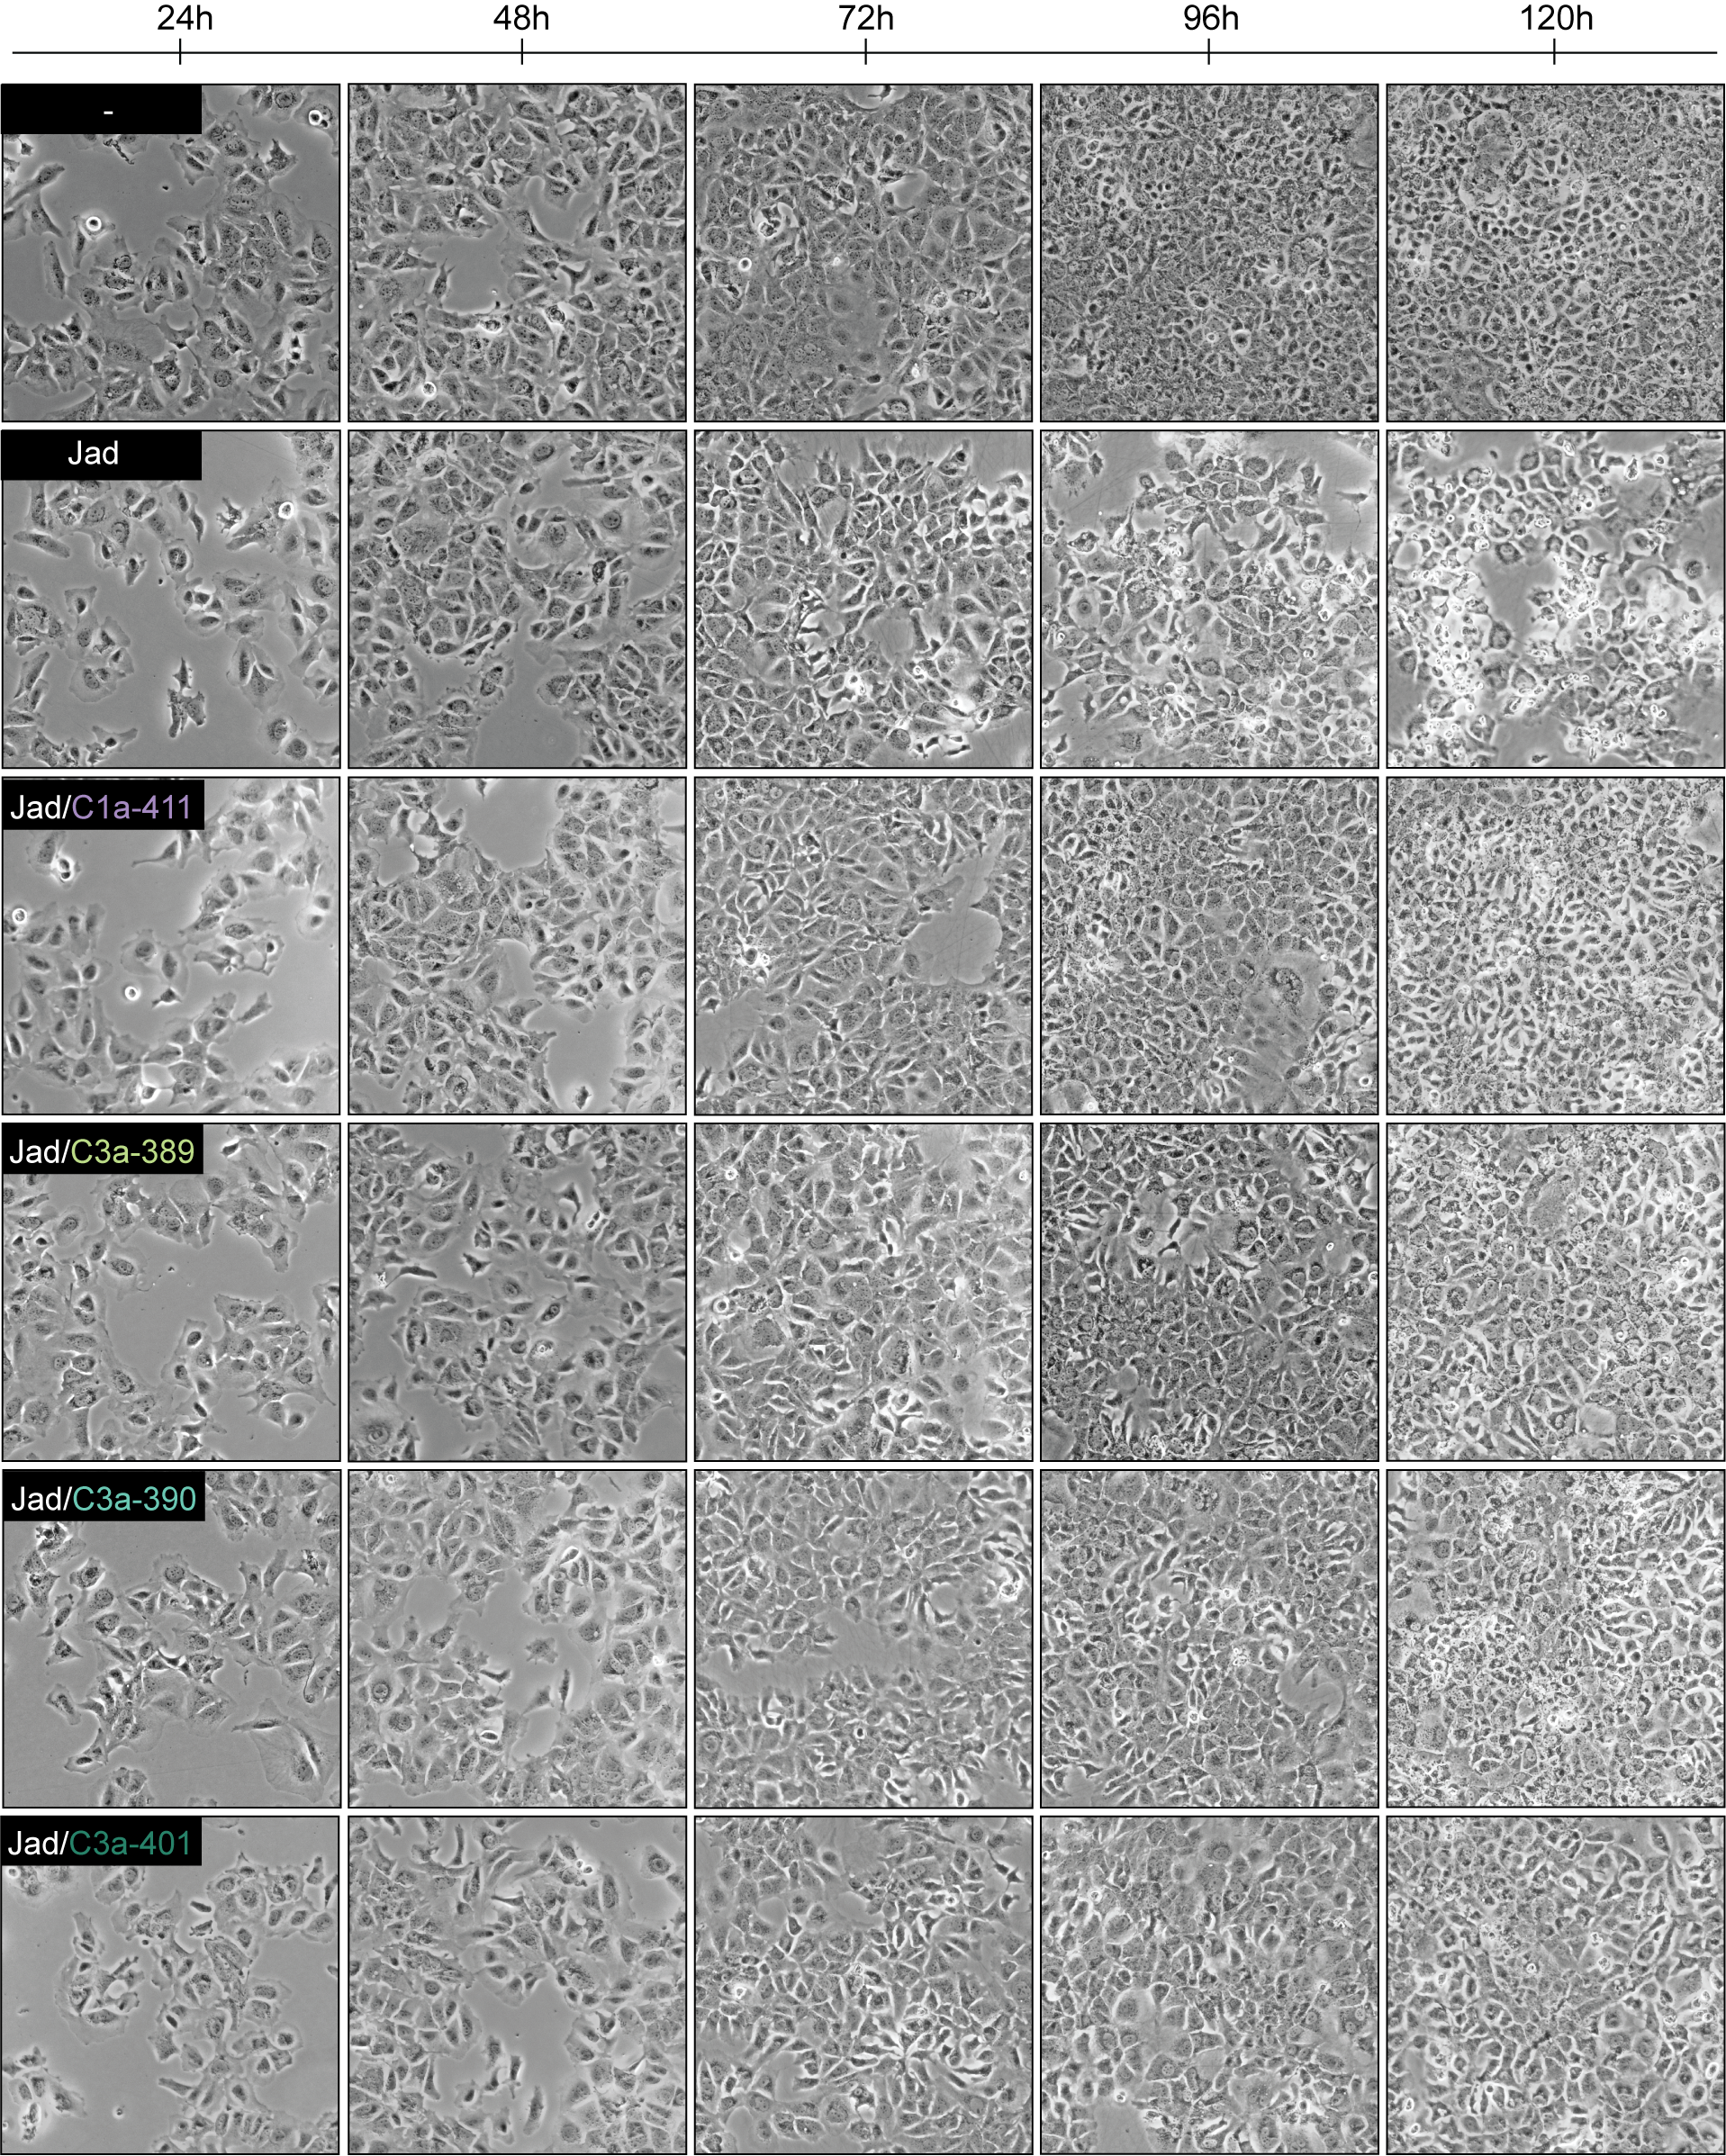
\includegraphics[width=\linewidth]{Figure_60.png}
		\caption[Suivi du profil morphologique des cultures d’hépatocytes naïfs et d’hépatocytes infectés par la souche parentale Jad ou par les virus intergénotypiques]{\textbf{Suivi du profil morphologique des cultures d’hépatocytes naïfs et d’hépatocytes infectés par la souche parentale Jad ou par les virus intergénotypiques.} Images des tapis cellulaires au cours d’une expérience de cinétique, de 24 à 120h p.i., obtenues par microscopie à champ lumineux ou « bright field » au grossissement 10X. Les images des cultures naïves (-) sont situées dans le panneau du haut et les images des cultures infectées par la souche parentale Jad ou par les virus recombinants indiqués sont montrés en dessous.}
				\label{fig:fig60}
	\end{figureth}
	\FloatBarrier

Les analyses quantitatives de l’étude cinétique sont représentées dans la \Autoref{fig:fig61}, et séparées arbitrairement en deux groupes de virus, afin de faciliter la lecture des représentations graphiques. Les données proviennent de six expériences indépendantes réalisées au fil de l’obtention des différents virus recombinants et ont été normalisées par rapport au contrôle parental inclus au sein de chaque expérience. Cette opération permet de s’affranchir de la variabilité entre expériences provenant principalement de la permissivité des lots de cellules utilisés pour l’infection et \textit{in fine} de comparer les paramètres de l’ensemble des virus recombinants. Les ARN viraux intracellulaires et extracellulaires ont été quantifiés après rétro-transcription et PCR quantitative en temps réel (RT-qPCR), avec un seuil de 50 à 100 copies selon les lectures. Pour s’affranchir des variations de dépôt, les ARN viraux intracellulaires quantifiés par µg d'ARN total ont été normalisés à partir de la quantité d’ARN 18S mesurée au sein du même échantillon. \\ \\
\indent
Les valeurs des ARN intracellulaires mesurés à 4h p.i. se situent autour de 10\up{6} à 10\up{7} copies/µg ARN total pour tous les virus, indiquant que l’efficacité d’entrée est similaire pour les virus recombinants et la souche parentale (\autoref{fig:fig61}\textcolor{blue}{.A}). On note une réduction globale de 0,5 à 1 log du niveau d'ARN viral intracellulaire à 12h p.i., indiquant que la réplication génomique n’a pas encore pris le pas sur la dégradation des génomes introduits à ce temps p.i. À partir de 24h p.i., on détecte une nette augmentation du niveau d’ARN intracellulaire accompagnée d’une synthèse de particules virales infectieuses pour l’ensemble des virus, indiquant que les étapes de réplication génomique, de morphogénèse et de sécrétion des virions s’initient entre 12 et 24h p.i. (\autoref{fig:fig61}\textcolor{blue}{.C}). Un cycle viral complet peut donc avoir lieu en 24h, mais le plateau de sécrétion des particules infectieuses est atteint à 72h ou 96h p.i., avec des titres de l’ordre de 1 à 5x10\up{5} TCID50/mL. Les cinétiques de réplication ont un profil relativement similaire entre les virus recombinants et la souche parentale, tant au niveau de l’ARN intracellulaire, de l’ARN extracellulaire que du titre viral. Toutefois, on note une production virale légèrement plus rapide et plus importante pour la plupart des recombinants que pour le parent Jad, à l’exception notable des virus Jad/C1aH77 et Jad/C1a-411. Ces résultats indiquent une efficacité d’assemblage et/ou de sécrétion de particules virales optimisée avec les séquences Core de génotype 3a ou 4, à l’inverse de celles de génotype 1a. On note également que le virus Jad/C3a-376 issus des passages tardifs des expériences d’adaptation montre une cinétique de réplication et un titre viral similaires aux autres virus recombinants codant les séquences de génotype 3a. Ces résultats soulignent le succès des tentatives d’adaptation de ce virus intergénotypique, initialement peu robuste.

			\begin{figureth}
	\centering
			\includegraphics[width=0.80\linewidth]{Figure_61.png}
		\caption[Cinétique de réplication des virus intergénotypiques dérivés du contexte génomique Jad]{\textbf{Cinétique de réplication des virus intergénotypiques dérivés du contexte génomique Jad.} \textit{La légende de la figure est décrite sur la page suivante \footnotemark[4].}}
	\label{fig:fig61}
	\end{figureth}
	\FloatBarrier
	
\footnotetext[4]{Mesure de (A) l’ARN viral intracellulaire par µg d’ARN total évalué par rapport à la quantification en temps réel d’ARN 18S (en log copies/µg d’ARN total), (B) l’ARN viral extracellulaire (en log copies/mL), (C) le titre viral infectieux (en log TCID50/mL) au cours de l’infection. Chaque virus a été analysé au cours de deux expériences indépendantes, chacune en duplicats. Les valeurs représentées sur les graphiques sont calculées relativement aux valeurs obtenues par Jad dans chaque expérience et exprimées par rapport aux valeurs moyennes obtenues sur l’ensemble des expériences. La souche de référence Jad est représentée par des courbes en pointillés noirs. Les tests statistiques ont été réalisés sur R à l’aide d’un modèle mixte linéaire, à partir des données brutes afin d’éviter les biais de la normalisation. Les \textit{p-values} situées dans les cadres en bas à droite des différents graphiques, indiquent les différences significatives de l’évolution des virus intergénotypiques par rapport au contrôle parental : significativement supérieur (en rouge) et significativement inférieur (en bleu). Les \textit{p-values} ont été ajustées par la méthode de Tukey : p <0,05 (*); p <0,01 (**); p <0,001 (***); p <0,0001 (****).}

Pour finir, j’ai comparé l’infectiosité spécifique de tous les virus recombinants et de la souche parentale Jad en calculant le ratio entre les particules virales infectieuses (TCID50) et les particules virales totales sécrétées (copies) (\autoref{fig:fig62}). Les ratios à 4h p.i. et 12h p.i. ne sont pas représentés car pas biologiquement pertinents en l’absence de néosynthèse de particules virales. On ne discerne pas de profil particulier en matière d’infectiosité spécifique entre les différents virus, quel que soit le temps p.i. On note toutefois une infectiosité spécifique légèrement supérieure pour les virus recombinants Jad/C3a-311, Jad/C3a-376 et plus faible pour les virus recombinants Jad/C2a-J6 et Jad/C4fC. On évalue à 250 à 1000 fois l’excès de particules non infectieuses selon les virus, ce qui est cohérent avec les ratios observés en culture cellulaire pour les recombinants J6(C-NS2)/JFH-1 décrits dans la littérature \citep{RN343}.

			\begin{figureth}
	\centering
			\includegraphics[width=\linewidth]{Figure_62.png}
		\caption[Comparaison de l’infectiosité spécifique des virus intergénotypiques dérivés du contexte génomique Jad]{\textbf{Comparaison de l’infectiosité spécifique des virus intergénotypiques dérivés du contexte génomique Jad.} L’infectiosité spécifique représente le ratio de particules virales infectieuses (TCID50) et de particules totales présentes dans le surnageant de culture (copies d’ARN).}
				\label{fig:fig62}
	\end{figureth}
	\FloatBarrier

\subsubsection{Analyse de la propagation des virus intergénotypiques exprimant les protéines Core hétérologues dans le contexte génomique Jad}

Afin de compléter la caractérisation des virus intergénotypiques, j’ai comparé leur propagation au sein des cultures cellulaires infectées par rapport à la souche parentale par microscopie confocale. Pour ce faire, la proportion de cellules positives pour une protéine virale 24, 48, 72 et 96h après infection avec les virus correspondants à 1 TCID50/cellule a été évaluée manuellement par microscopie confocale (\autoref{fig:fig63}\textcolor{blue}{.A}). Afin de ne pas biaiser l’évaluation, la protéine NS5A commune à tous les virus a été choisie pour cette étude. Le signal obtenu pour NS5A est très intense et relativement homogène, ce qui rend facilement identifiable les cellules infectées (\autoref{fig:fig63}\textcolor{blue}{.B}). Au sein des cellules infectées, NS5A est uniformément distribuée dans le cytoplasme, ce qui est compatible avec une localisation au niveau du RE. On observe parfois des puncta intenses à proximité des GL à partir de 48h p.i., signant une concentration transitoire de la protéine dans des régions précises. Ces structures pourraient être attribuables aux sites de réplication génomique ou d’assemblage des particules virales, comme il a été suggéré lors d’une étude par microscopie électronique basée sur un réplicon sous-génomique codant la protéine NS5A fusionnée à la GFP \citep{RN985} ou de travaux sur la dynamique de NS5A-GFP en cellules vivantes infectées par la souches Jc1 \citep{RN983}. Pour estimer la proportion de cellules infectées par rapport au nombre total de cellules, le noyau a été révélé à l’aide du DAPI. Cette estimation a été réalisée à partir de 5 à 7 champs de cellules, comptabilisant en moyenne 500 à 700 cellules au cours de deux expériences indépendantes. Les proportions représentées ont été normalisées par rapport au contrôle parental respectif.

			\begin{figureth}
	\centering
			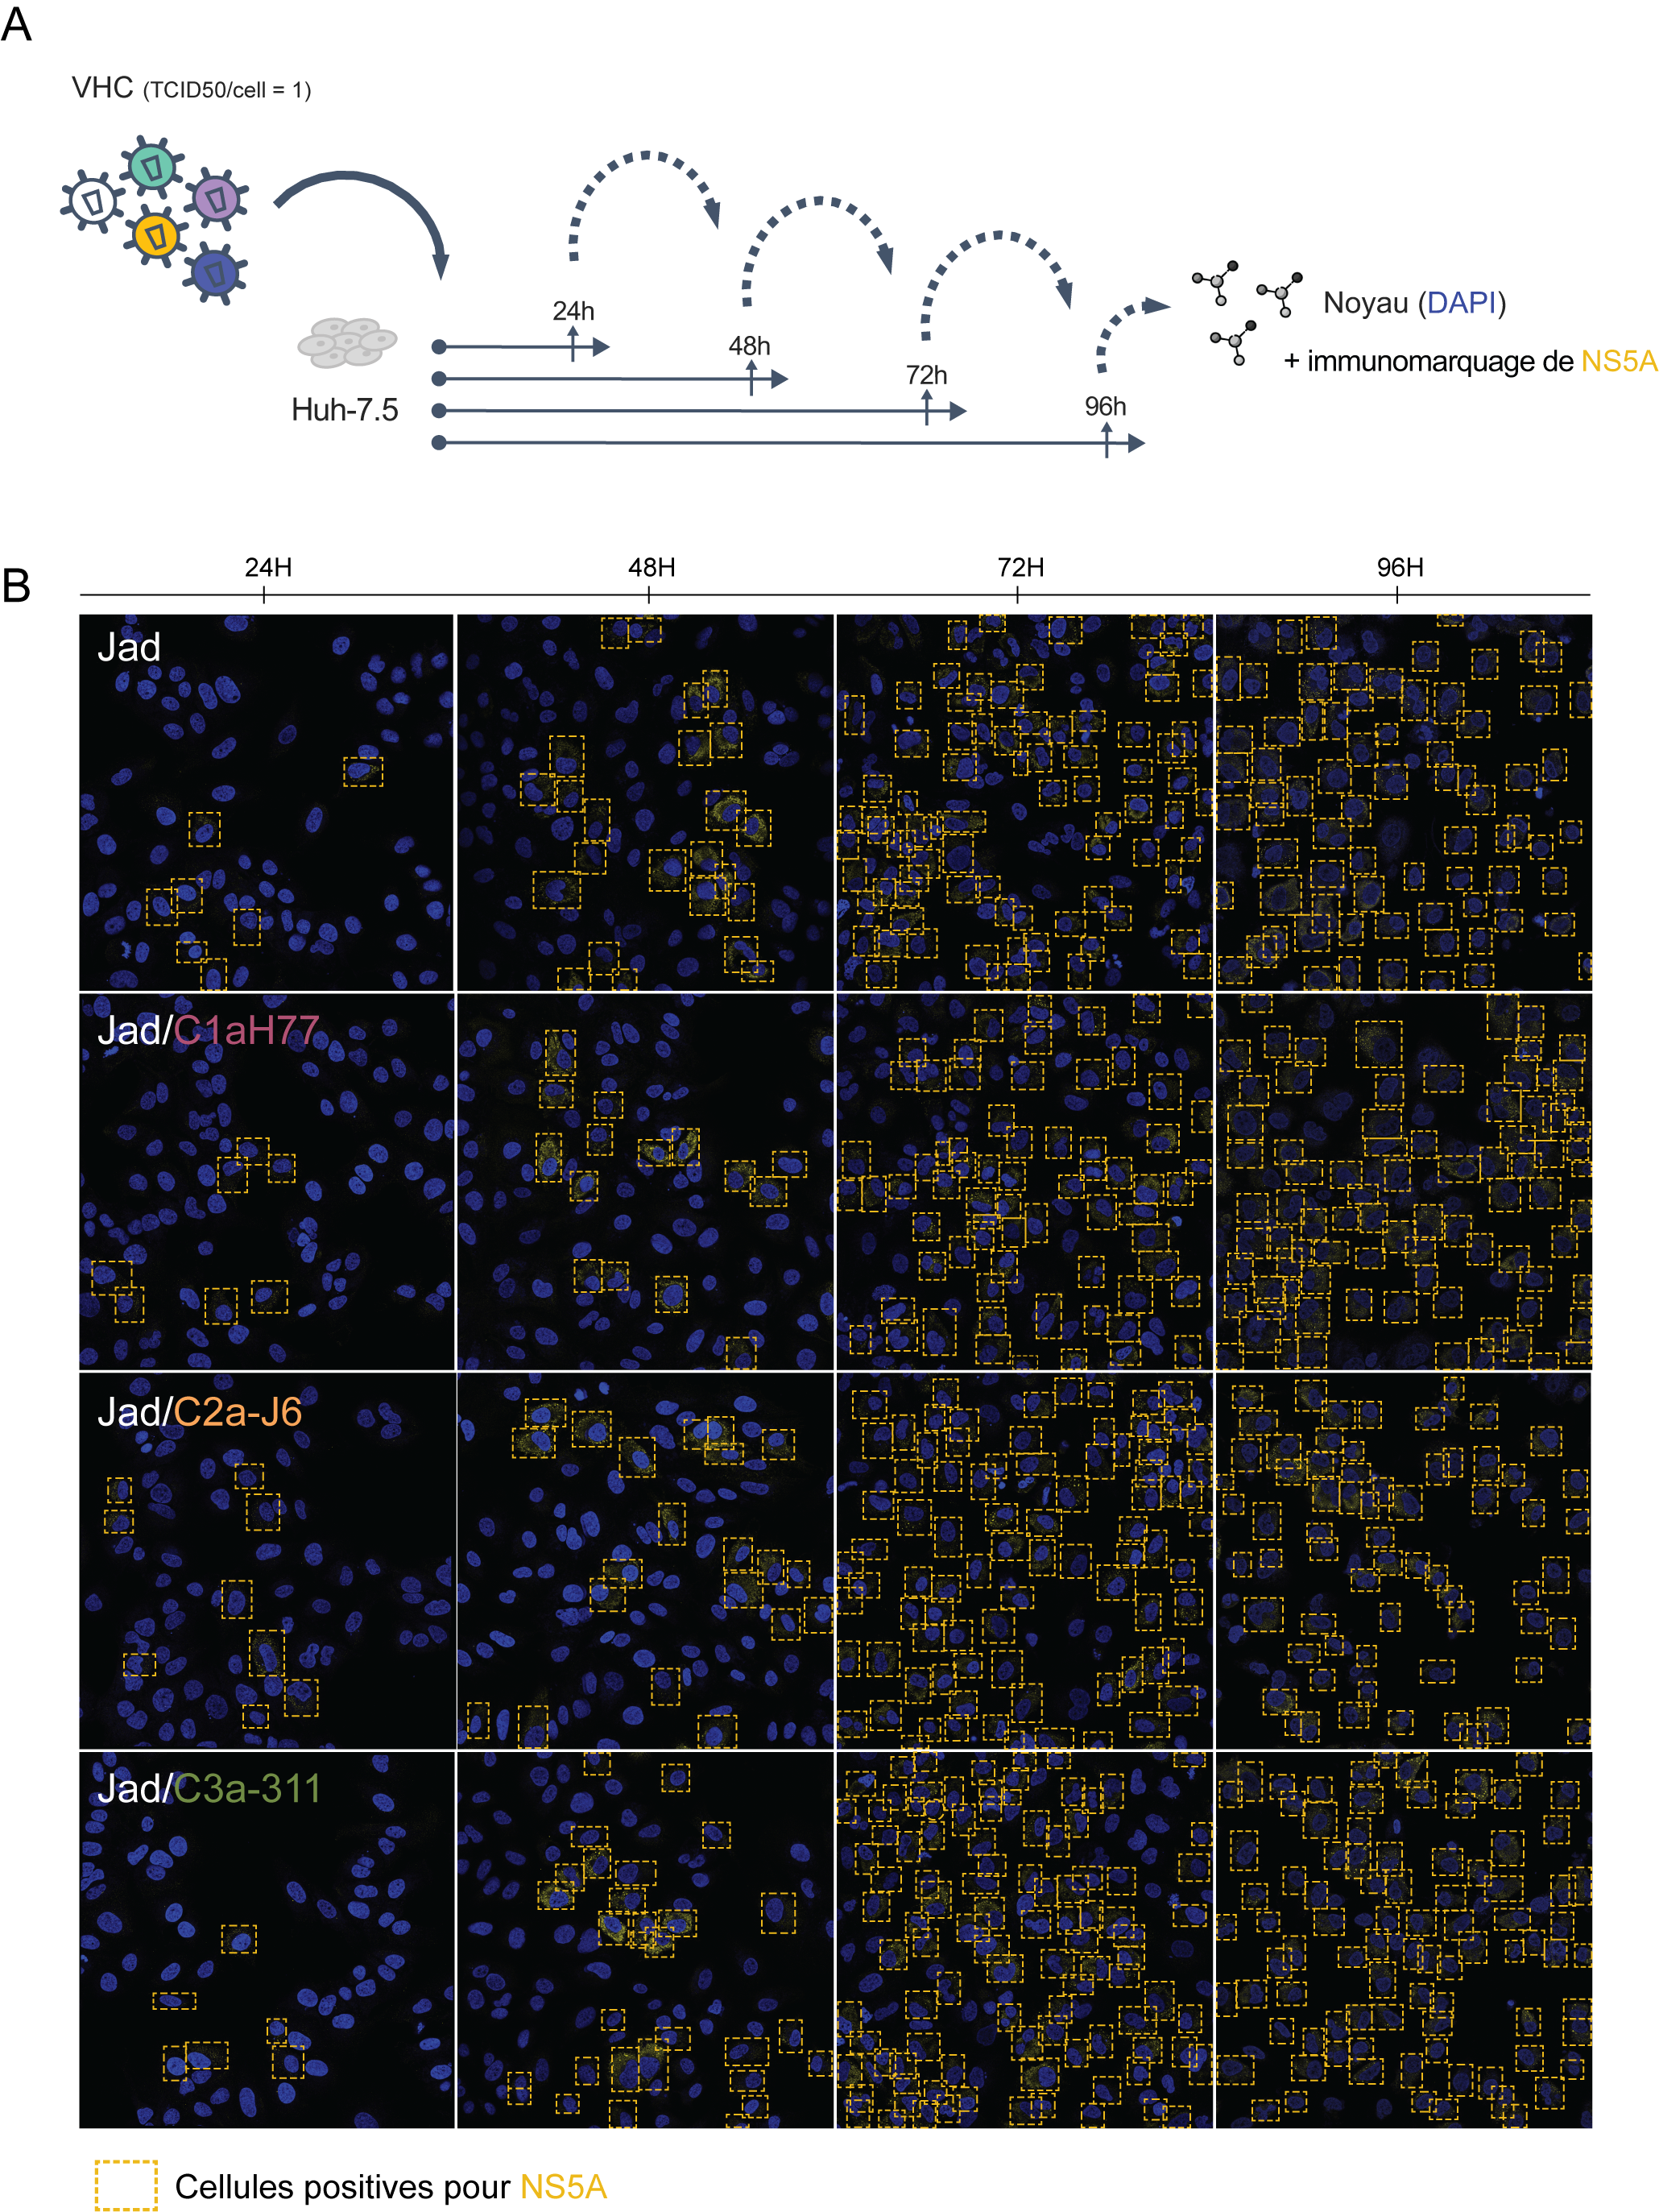
\includegraphics[width=\linewidth]{Figure_63.png}
		\caption[Propagation des virus intergénotypiques dérivés du contexte génomique Jad par microscopie confocale (Partie 1)]{\textbf{Propagation des virus intergénotypiques dérivés du contexte génomique Jad par microscopie confocale (Partie 1).} (A) Schéma simplifié de l’approche expérimentale pour analyser la propagation des virus intergénotypiques au cours de l’infection. Des cellules Huh-7.5 ont été infectées par les différents virus intergénotypiques ou la souche parentale Jad à une MOI de 1 TCID50/cellule et fixées à 24, 48, 72 ou 96h p.i. (B) Champs représentatifs de cellules Huh-7.5 infectées par différents virus aux temps p.i. indiqués, obtenus par projection d’intensité maximale. La protéine virale NS5A a été révélée par immunomarquage (en jaune) et les noyaux cellulaires par incorporation du DAPI (en bleu). Les cellules comportant un signal positif pour NS5A sont mises en évidence par des cadres jaunes pointillés.}
				\label{fig:fig63}
	\end{figureth}
	\FloatBarrier

Le taux de cellules positives pour NS5A augmente progressivement au cours de l’infection, de manière similaire pour le virus parental et la plupart des virus recombinants, à l'exception notable de Jad/C4aR et Jad/C4fC qui se propagent plus rapidement (\autoref{fig:fig64}). À 24h p.i, entre 5 et 15\% des cellules sont positives pour NS5A pour la souche parentale et les virus intergénotypiques codant les protéines Core 1aH77, 2a-J6, 3a-311, 3a-376 et 3a-395, alors que cette proportion est de 30 à 35\% pour les virus intergénotypiques codant les protéines Core 4aR et 4fC. Ces derniers ont colonisé environ 75\% des cellules dès 48h p.i., puis atteint 95\% des cellules dès 72h p.i. La souche parentale ainsi que les autres virus recombinants atteignent un taux d’infection à hauteur de 70 à 80\% à 72h p.i., qui augmente légèrement jusqu’à atteindre 80 à 95\% de cellules infectées à 96h p.i. On peut noter que la quasi-totalité des cellules sont infectées par tous les virus parental et intergénotypiques à 96h p.i. dans des conditions d’infection initiales à 1 TCID50 / cellule. Ainsi, ces résultats démontrent que les virus intergénotypiques ont une efficacité de dissémination similaire, voire supérieure (Jad/C4aR et Jad/C4fC) à celle de la souche parentale. La diffusion plus dynamique des virus recombinants Jad/C4aR et Jad/C4fC entre 24h et 72h p.i. est cohérente avec les données issues de la cinétique de réplication, soulignant encore une fois la performance des virus intergénotypiques codant les protéines Core de génotype 4. Cette analyse n’a pas encore été étendue à tous les virus intergénotypiques et il serait intéressant de la compléter pour les virus recombinants codant core de génotype 3a qui ont également montré une cinétique de réplication légèrement plus rapide (Jad/C3a-389, Jad/C3a-390 et Jad/C3a-401). Par ailleurs, la proportion entre la distribution de NS5A strictement « réticulée » et la distribution en puncta est du même ordre de grandeur pour les différents virus, montrant que la substitution de Core n’a pas d’impact significatif sur la localisation de la protéine virale NS5A.
	\vfill
			\begin{figureth}
	\centering
			\includegraphics[width=\linewidth]{Figure_64.png}
		\caption[Propagation des virus intergénotypiques dérivés du contexte génomique Jad par microscopie confocale (Partie 2)]{\textbf{Propagation des virus intergénotypiques dérivés du contexte génomique Jad par microscopie confocale (Partie 2).} Estimation des proportions de cellules positives pour NS5A au sein du tapis cellulaire infecté par la souche parentale Jad ou par les différents virus intergénotypiques testés. L’analyse a été conduite sur 5 à 7 champs de cellules, dans deux expériences indépendantes. Les proportions sont calculées relativement aux valeurs obtenues pour la souche parentale au sein de chaque expérience et exprimées par rapport aux valeurs moyennes inter-expériences du parent.}
				\label{fig:fig64}
	\end{figureth}
	\FloatBarrier
	\vfill
	\clearpage

Pour conclure ce chapitre, l’ensemble de ces résultats montre que la substitution de la protéine Core du JFH-1 par des protéines Core hétérologues de divers génotypes n’affecte pas de façon majeure les étapes de traduction, réplication génomique et morphogénèse virale, à l’exception d’une seule séquence de génotype 3a. Un virus intergénotypique résultant de l’insertion de cette dernière séquence (Jad/C3a-376) aussi robuste que la souche parentale et sans altération de la séquence Core initiale a néanmoins pu être sélectionné. Nous avons donc généré un large éventail de virus intergénotypiques uniques qui se propagent et se répliquent à un niveau et selon une cinétique similaires à ceux de la souche prototypique parentale, ce qui permet d’effectuer des analyses comparatives dans les cellules d'hépatome infectées.

		\subsection{Analyse du profil et de la localisation intracellulaire des protéines Core hétérologues exprimées par les virus intergénotypiques}
		\label{section:localisation}

Pour réaliser l’étude du profil et de la localisation des protéines Core hétérologues vis-à-vis des GL, il était nécessaire d’avoir un anticorps monoclonal dit « pan-génotypique », c’est-à-dire capable de reconnaître avec la même affinité les variants de Core, indépendamment de leur origine génotypique. Plusieurs anticorps monoclonaux ciblant la protéine Core du VHC ont été commercialisés, la plupart contre les protéines Core des souches prototypiques disponibles, telles que JFH-1 de génotype 2a, H77 de génotype 1a ou encore Con1 de génotype 1b. En sachant que les séquences de Core de génotype 3a sont relativement distantes des séquences de génotypes 2a et 1a (voir \autoref{section:souches}) et que ces protéines pouvaient présenter des différences conformationnelles, l’efficacité de reconnaissance de ces protéines par ces anticorps commerciaux pouvait être affectée.

	\subsubsection{Evaluation de la capacité d’anticorps monoclonaux à reconnaître les protéines Core hétérologues de différents génotypes}
	
Dans un premier temps, j’ai testé plusieurs anticorps monoclonaux commerciaux produits chez la souris : l’anticorps 1851 ciblant la protéine Core de la souche H77, les anticorps 4F5 et 3D11 ciblant la protéine Core de la souche JFH-1 et l’anticorps C7-50 ciblant la protéine Core de la souche Con1 (voir \autoref{tab:tabM1}). En parallèle, notre laboratoire a obtenu deux solutions d’anticorps non commercialisés : un anticorps monoclonal ACAP27 produit chez la souris contre la protéine Core de la souche H77 donné généreusement par A. Budkowska (Institut Pasteur) et des anticorps polyclonaux (FL) produits chez le lapin immunisé avec la protéine Core de cette même souche, donnés généreusement par A. Kakkanas (\textit{Hellenic Pasteur Institute, Athens, Greece}). En théorie, les anticorps polyclonaux FL devraient reconnaître efficacement tous les variants de Core, compte tenu de la présence de régions très conservées entre les séquences, et donc de la grande probabilité d’avoir des épitopes en commun. Ce sérum était donc précieux pour contrôler et comparer l’expression et la stabilité des protéines Core hétérologues produites par les virus intergénotypiques. \\ \\
\indent
Cette panoplie d’anticorps a été testée sur des lysats protéiques collectés à partir de cellules Huh-7.5 infectées par les différents virus intergénotypiques ou par la souche parentale à 96h p.i. Cette échéance tardive a été choisie afin de limiter les différences en production de protéines virales, qui pourraient survenir lorsque les cinétiques de réplication virale ne sont pas parfaitement synchrones. Des immunoblots révélés par fluorescence dans le proche infrarouge ont permis de quantifier l’expression de la protéine virale Core. Ce système fluorescent permet en effet d’effectuer une quantification fiable et linéaire du signal jusqu’à un seuil de saturation du détecteur \citep{RN981} et de renseigner sur les différences fines d’abondance entre les différentes protéines Core. Les variations de dépôts étant fréquentes pour ce type d’approche expérimentale, il est nécessaire de normaliser systématiquement le signal de Core par rapport à une référence cellulaire invariable pour lisser les variations de dépôts des protéines totales. C’est d’autant plus important que l’infection ralentit la croissance cellulaire et que seule a souche parentale induit une mortalité cellulaire très élevée à 96h p.i. (voir \autoref{section:virus}). Les protéines virales n’atteignaient jamais le seuil de saturation du détecteur et leur signal figurait toujours dans la gamme linéaire de détection. En revanche, l’actine ß étant trop abondante, le signal a tendance à atteindre le plateau de détection. Ainsi, l’actine ß ne constitue pas un bon candidat pour la normalisation quantitative des dépôts et fera seulement office de contrôle visuel des extraits. À la place, les protéines totales ont été quantifiées après révélation avec une solution REVERT (Li-Cor), compatible avec ce système de détection par fluorescence \citep{RN980,RN979}. La protéine virale NS5B, commune à l’ensemble des virus, a été révélée en guise de contrôle visuel du niveau d’infection.

			\begin{figureth}
	\centering
			\includegraphics[width=\linewidth]{Figure_65.png}
		\caption[Evaluation de l’efficacité de reconnaissance des protéines Core exprimées par les virus intergénotypiques par différents anticorps monoclonaux et polyclonaux]{\textbf{Evaluation de l’efficacité de reconnaissance des protéines Core exprimées par les virus intergénotypiques par différents anticorps monoclonaux et polyclonaux.} (A, C, E) Les protéines totales extraites à 96h p.i. des cellules Huh7.5 infectées avec les virus intergénotypiques ou avec la souche parentale ont été séparées par électrophorèse SDS-PAGE. La détection des protéines virales NS5B et Core et de l’actine ß sont montrées séparément. L’anticorps utilisé pour révéler la protéine Core est indiqué en bas de chaque panneau. Les marqueurs de masses moléculaires (kDa) sont indiqués à droite des images. (B, D, F) Analyse quantitative de l’abondance relative des protéines Core hétérologues (barres colorées) par rapport à la protéine native (barre noire). Les valeurs d’intensité du signal de Core ont été normalisées par rapport aux protéines totales révélées par la solution REVERT. Les graphiques représentent des moyennes et écart-types issus de 2 à 3 séries d’immunoblots indépendantes. Le seuil de 100\% (ligne pointillée) est établi à la valeur moyenne de Jad/C1aH77, protéine contre laquelle les anticorps 1851, FL et ACAP27 ont été produits.}
				\label{fig:fig65}
	\end{figureth}
	\FloatBarrier

Comme attendu, le signal détecté par l’anticorps polyclonal est élevé pour toutes les protéines Core exprimées par les virus intergénotypiques, confirmant un spectre élargi à tous les génotypes (\autoref{fig:fig65}\textcolor{blue}{.A}). L’analyse quantitative révèle toutefois une abondance relative de 40 à 60\% par rapport à la protéine Core de la souche parentale pour toutes les protéines Core exprimées par les virus intergénotypiques, suggérant que les variants de Core seraient moins stables que la protéine native à 96h p.i. (\autoref{fig:fig65}\textcolor{blue}{.B}). Le signal détecté par l’anticorps 1851 est élevé pour la protéine Core 1a-H77 contre laquelle il a été produit, y compris pour pour l’autre protéine Core de génotype 1a (1a-411) et pour les protéines Core de génotype 2 (JFH-1, J6) (\autoref{fig:fig65}\textcolor{blue}{.C-D}). En revanche, le signal détecté pour les protéines Core de génotype 3a est diminué de ~80 à 90\%, et dans une moindre mesure, de ~50\% pour les protéines Core de génotype 4. Ce résultat démontre que l’anticorps monoclonal 1851 ne reconnaît pas efficacement les protéines Core de génotype 3a. Les autres anticorps monoclonaux commerciaux 4F5, 3D11 et C7-50 ne reconnaissent pas non plus les protéines Core de génotype 3a et l’anticorps 3D11 s’est avéré de plus incapable de reconnaître les protéines Core de génotype 4 (résultats non montrés). En revanche, l’anticorps monoclonal ACAP27 montre un profil étendu à l’ensemble des protéines Core hétérologues, y compris les protéines Core de génotype 3a (\autoref{fig:fig65}\textcolor{blue}{.E-F}). \\ \\
\indent
Ces résultats peuvent s’expliquer par les variations de séquences au sein des épitopes cibles des anticorps, lorsque ceux-ci sont connus. Cette recherche n’a pas été totalement fructueuse et seuls les épitopes des anticorps 1851, C7-50 et ACAP27 m’ont été renseignés (\autoref{fig:fig66}). L'épitope ciblé par les anticorps 1851 et C7-50 correspondant aux résidus 30 à 40 est identique pour les souches considérées de génotypes 1a, 1b, 2a ou 4 mais contient une valine en position 36 au sein de toutes les séquences de génotype 3. Ce résidu unique au génotype 3 pourrait être la cause de la faible affinité de ces anticorps pour les protéines Core appartenant à ce génotype.  L’épitope ciblé par ACAP27 est plus large (résidus 39 à 72) et bien conservé pour la grande majorité des souches. Les quelques mutations naturelles présentes dans certaines séquences de Core, notamment de génotype 2a, n’apparaissent pas gêner l’efficacité de reconnaissance par l’anticorps ACAP27 par immunoblot. Il a ensuite été vérifié que ces conversions n'affectent pas non plus l’efficacité de reconnaissance de l'épitope conformationnel par l’anticorps ACAP27 en conditions natives, lors des analyses d’imagerie par immunofluorescence.

			\begin{figureth}
	\centering
			\includegraphics[width=\linewidth]{Figure_66.png}
		\caption[Alignement partiel des séquences protéiques de Core des souches prototypiques et des souches cliniques]{\textbf{Alignement partiel des séquences protéiques de Core des souches prototypiques et des souches cliniques.} Seuls les acides aminés en positions 1 à 80 de Core sont affichés. Les séquences sont classées selon le génotype de leur souche d’origine. Les nucléotides identiques sont représentés par des points noirs. Les nucléotides les plus communs sont de couleur noire et les résidus les moins communs sont de couleur rouge. Des cadres pointillés indiquent l’épitope cible connu des anticorps monoclonaux.}
				\label{fig:fig66}
	\end{figureth}
	\FloatBarrier

En conclusion, ces analyses comparatives démontrent qu’il n’est pas judicieux d’utiliser les anticorps monoclonaux commerciaux produits contre les protéines Core de JFH-1 ou Con1 pour étudier notre panel de virus intergénotypiques, en raison de leur manque d’efficacité à reconnaître les protéines Core de génotype 3. En revanche, l’anticorps ACAP27 présente une spécificité croisée satisfaisante pour les protéines Core de génotypes 1, 2, 3 et 4. Cet anticorps a donc été sélectionné pour la suite de l’étude. De plus, grâce à des anticorps polyclonaux, j’ai mis en évidence que les protéines Core hétérologues ont une stabilité inférieure à la protéine native, sans affecter de façon notable l’efficacité de réplication et de production des virus intergénotypiques (voir \autoref{section:virus}).

	\subsubsection{Analyse du profil et de la localisation intracellulaire des différentes protéines Core hétérologues au cours de l’infection}

Ayant à disposition deux anticorps « pan-génotypiques », l’anticorps monoclonal ACAP27 et les anticorps polyclonaux FL, le profil et la localisation des différentes protéines Core hétérologues vis-à-vis des GL on été comparés par microscopie confocale. Pour effectuer cette étude, des cellules Huh-7.5 ont été infectées par la souche parentale et par les différents virus intergénotypiques puis mises en contact pendant 15h avec du BODIPY avant d’être fixées à 24h, 48h, 72h et 96h p.i, selon l’approche expérimentale schématisée dans la \Autoref{fig:fig67}. La protéine Core a été révélée par immunofluorescence indirecte en utilisant les anticorps polyclonaux FL produits par le lapin et la protéine virale NS5A à l'aide d'un anticorps monoclonal produit chez la souris.

			\begin{figureth}
	\centering
			\includegraphics[width=\linewidth]{Figure_67.png}
		\caption[Schéma simplifié de l’approche expérimentale pour analyser le profil et la localisation intracellulaire des différents variants de Core]{\textbf{Schéma simplifié de l’approche expérimentale pour analyser le profil et la localisation intracellulaire des différents variants de Core.} Des cellules Huh-7.5 ont été infectées par la souche parentale Jad ou par les virus intergénotypiques à une MOI de 1 TCID50/cellule. Les GL ont été révélées par incorporation du BODIPY en cellules vivantes et les protéines virales NS5A et Core ont été révélées par immunomarquage à l’aide d’un anticorps monoclonal de souris et de l’anticorps polyclonal FL produit chez le lapin après fixation des cellules aux différents temps p.i indiqués.}
				\label{fig:fig67}
	\end{figureth}
	\FloatBarrier

Pour la souche parentale Jad, la proportion de cellules positives pour NS5A augmente graduellement à mesure que l’infection progresse, jusqu’à atteindre la quasi-totalité de la culture (\autoref{fig:fig68}\textcolor{blue}{.A}), comme observé précédemment dans le cadre de l’étude de la dissémination virale à la même MOI (voir \autoref{section:virus}). Au sein des cellules infectées, on retrouve l’aspect de NS5A majoritairement réticulée dans le cytoplasme avec une intensité de signal homogène. En revanche, à ce grossissement de champs d’une quarantaine de cellules, on s’aperçoit que le signal de Core est très hétérogène d’une cellule infectée à une autre, y compris aux temps tardifs, en dépit de la forte stabilité de la protéine native. On distingue des cellules avec un signal global de Core « intense », « modéré » ou « faible » voire inexistant, bien que le co-marquage de NS5A confirme l’infection de ces cellules (\autoref{fig:fig68}\textcolor{blue}{.B}). Pour évaluer l’hétérogénéité du marquage de Core au cours de l’infection, j’ai comptabilisé et catégorisé manuellement les cellules présentant un signal positif pour NS5A (définies comme infectées) en trois groupes, sur la base de cette estimation visuelle de l’intensité de Core (\autoref{fig:fig68}\textcolor{blue}{.C}). La majorité des cellules infectées présente un signal de Core « modéré » à 24h p.i., tandis qu’environ 8\% des cellules montrant un signal de Core « intense ». À partir de 48h p.i., on observe une forte augmentation de la proportion en cellules infectées présentant un signal « intense » de Core, jusqu’à environ 50\%. Ces proportions restent ensuite globalement stables à 72h p.i. et 96h p.i., indiquant qu’il n’y a pas de progression linéaire de l’intensité du signal de Core, contrairement à celle de NS5A. On peut d’ailleurs constater qu’une part non négligeable de cellules infectées présentent un signal faible voire inexistant pour Core, de l’ordre de 10 à 18\% à mesure que l’infection progresse.

			\begin{figureth}
	\centering
			\includegraphics[width=\linewidth]{Figure_68.png}
		\caption[Analyse de l’évolution des marquages de NS5A et de Core au cours du temps après infection par la souche parentale Jad]{\textbf{Analyse de l’évolution des marquages de NS5A et de Core au cours du temps après infection par la souche parentale Jad.} (A) Images représentatives de champs de cellules infectées par la souche parentale Jad aux temps p.i. indiqués. De haut en bas, les protéines virales NS5A et Core et les GL ont été révélées respectivement par l’anticorps monoclonal 4F5, les anticorps polyclonaux FL et le BODIPY. En dessous, figure la combinaison des marquages de NS5A, Core et des GL. Les barres d’échelle indiquent 50µm. (B) Zoom sur les images prises à 96h p.i., établissant les trois groupes d’intensité du signal de Core « Intense », « Modéré », « Faible / à peine visible » mis en évidence par des cadres en pointillés cyans, bleus ou magentas respectifs. (C) Estimation de la proportion en cellules infectées sur la base d’un signal positif pour NS5A, selon l’intensité du signal de Core aux différents temps p.i. indiqués. Les proportions ont été évaluées sur 500 à 700 cellules.}
				\label{fig:fig68}
	\end{figureth}
	\FloatBarrier

Le profil de Core dans les cellules infectées par les virus intergénotypiques a ensuite été comparé avec la souche de référence. La proportion de cellules détectées avec un signal de Core défini comme « intense » sur la base du parent est significativement plus faible pour l’ensemble des virus recombinants et atteint une valeur plafond de l’ordre de 10 à 15\% à 96h p.i. (\autoref{fig:fig69}), bien qu’à cette étape, un plateau de production virale similaire à la souche parentale soit atteint. La majorité des cellules infectées par les virus recombinants présentent un signal de Core « modéré », ainsi qu’une proportion plus importante de cellules avec un signal « faible » que la souche parentale, de l’ordre de 30\%. Ces proportions ont été précisément déterminées pour quelques virus intergénotypiques codant les protéines Core de génotype 1, 2 ou 3 (\autoref{fig:fig70}) et l’étude pourrait être élargie à l’ensemble des virus recombinants, en particulier aux virus codant pour les protéines Core de génotype 4. La faiblesse du signal de Core n’est vraisemblablement pas attribuable à des affinités différentes de l’anticorps polyclonal pour les variants de Core ou à des différences de dissémination virale, comme le démontre le co-marquage de la protéine NS5A et les analyses précédentes (voir \autoref{section:virus}). Ainsi, le faible signal de Core dans les cellules infectées par les virus intergénotypiques est probablement lié à une stabilité moindre des protéines Core hétérologues par rapport à la protéine native, ce qui est cohérent avec les analyses par immunoblot.

		\begin{figureth}
	\centering
			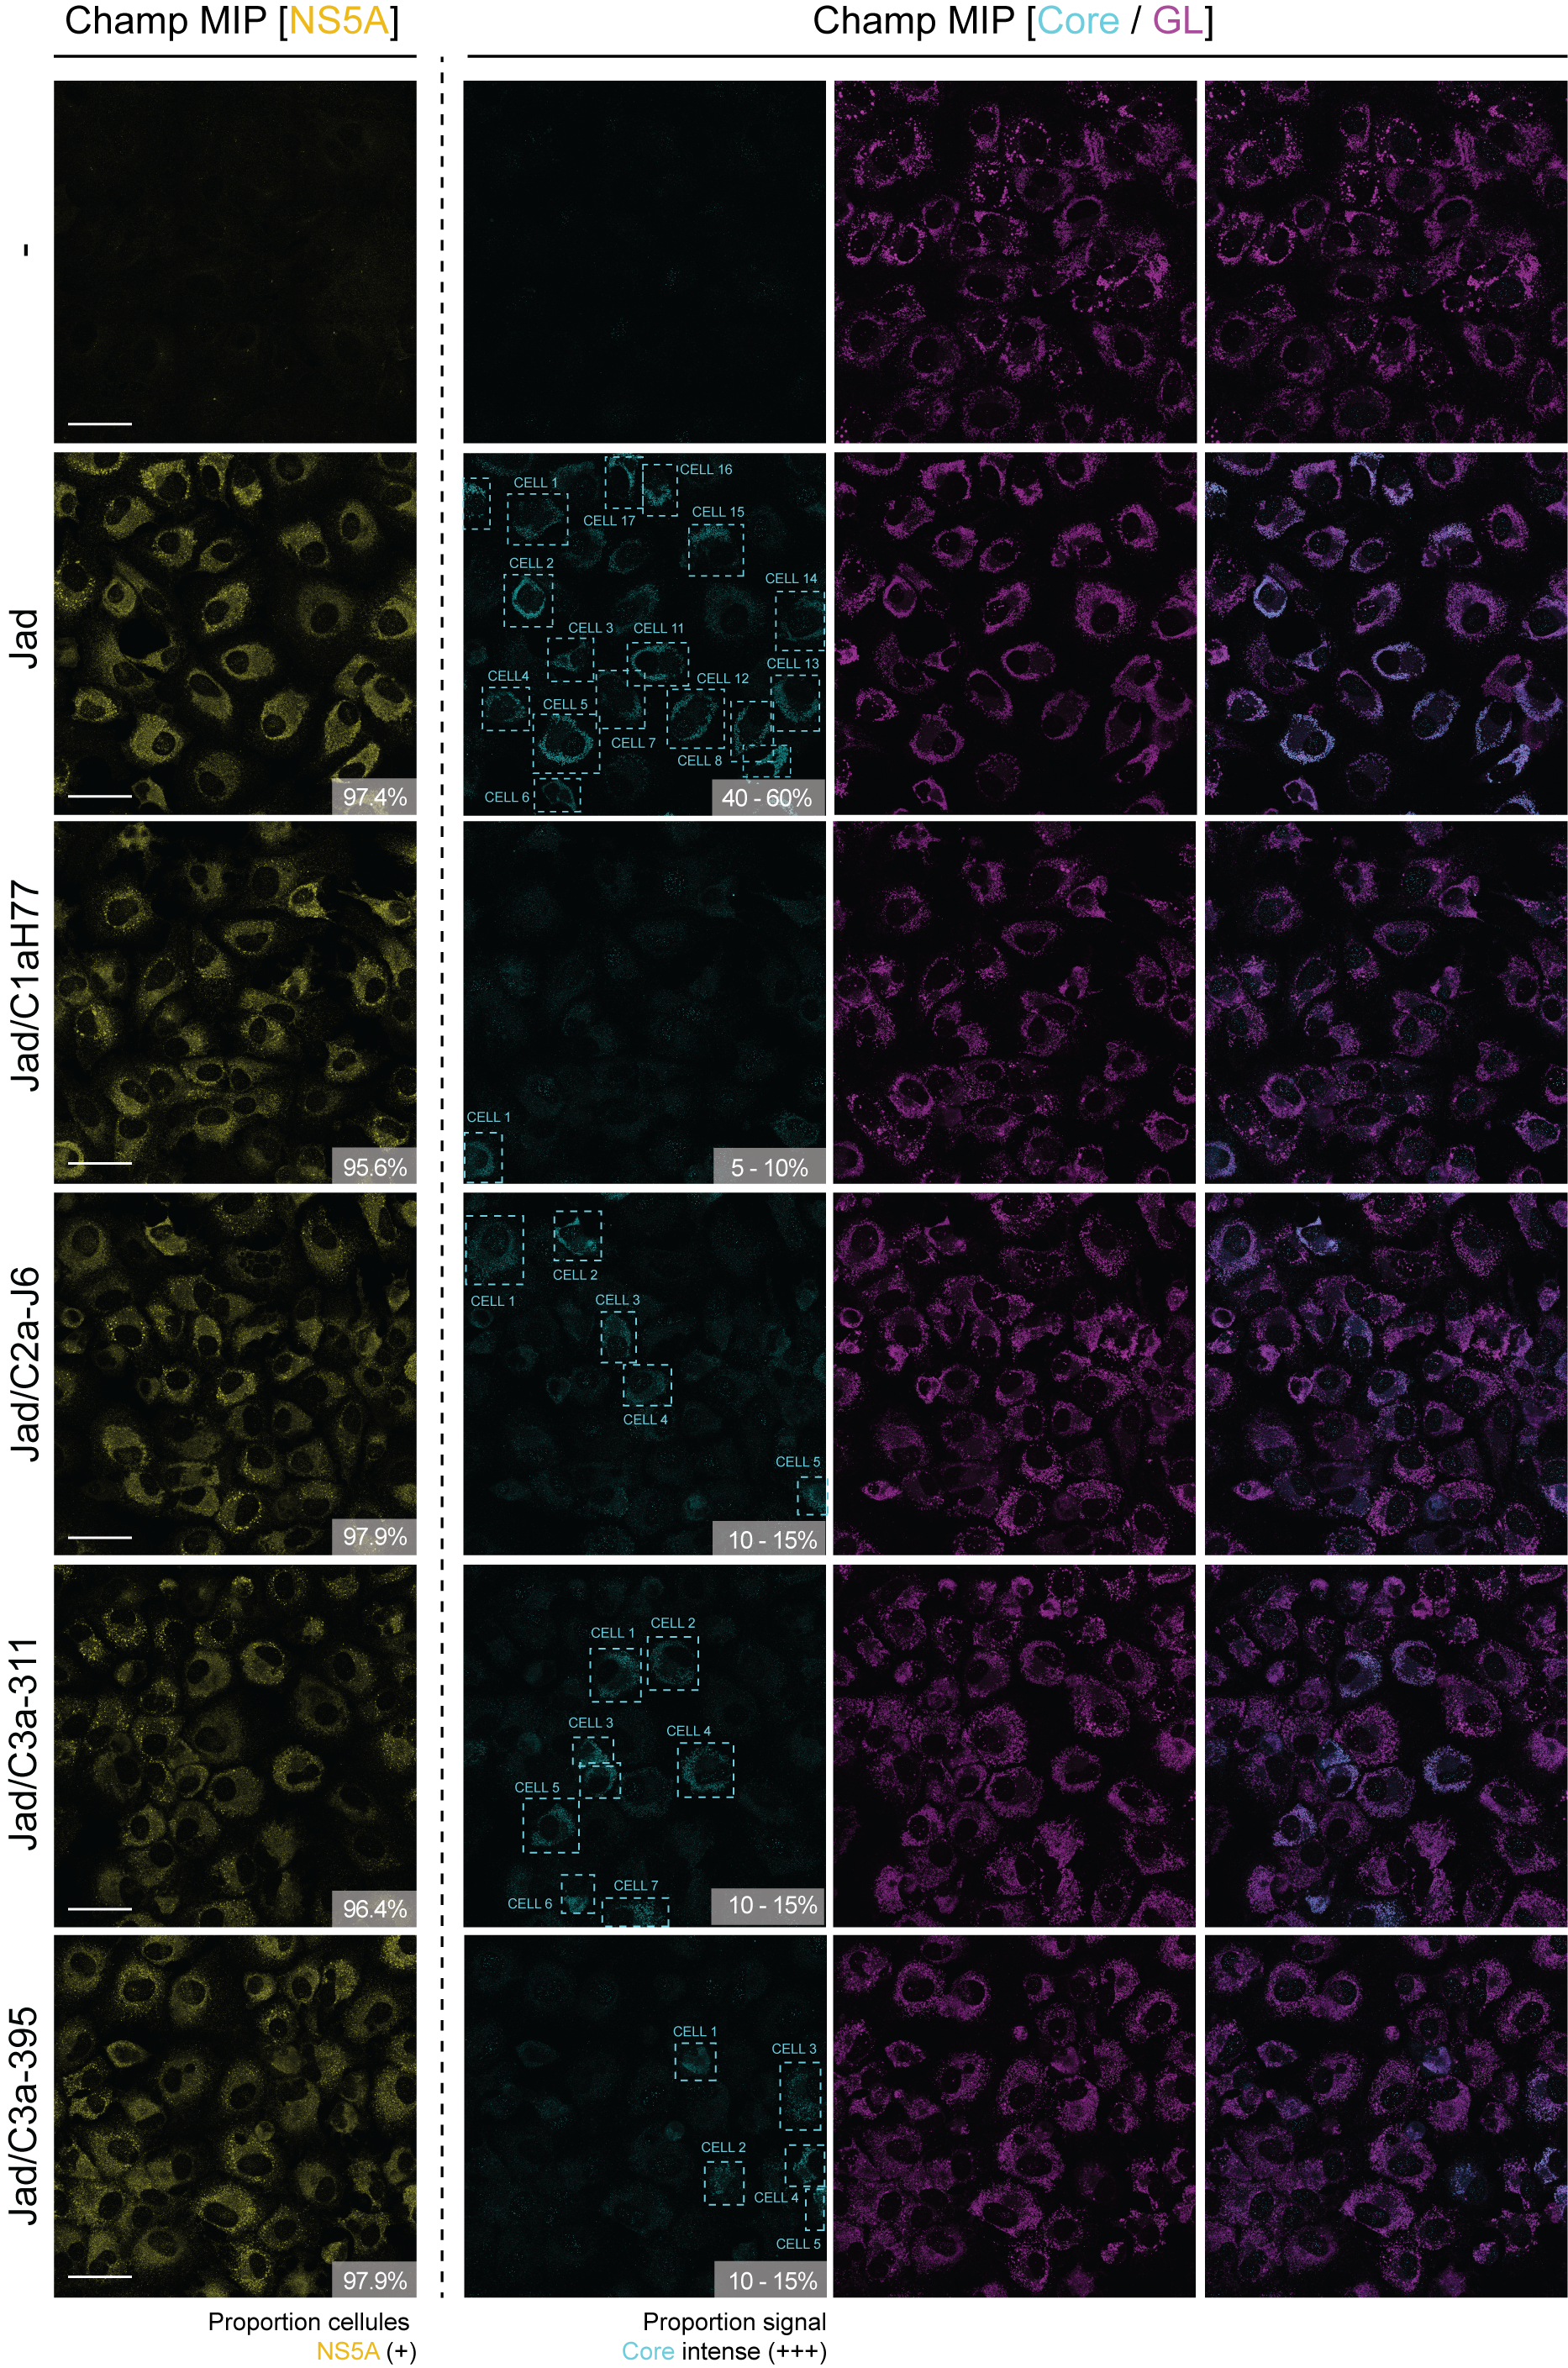
\includegraphics[width=0.80\linewidth]{Figure_69.png}
		\caption[Analyse de l’hétérogénéité du marquage de Core dans les cellules infectées par les virus intergénotypiques (Partie 1)]{\textbf{Analyse de l’hétérogénéité du marquage de Core dans les cellules infectées par les virus intergénotypiques (Partie 1).} Images représentatives 3D obtenues par MIP (ou \textit{Maximum Intensity Projection}) à 96h p.i. de champs de cellules non infectées ou infectées par la souche parentale Jad ou par quelques virus intergénotypiques. Dans le panneau de gauche figure la révélation de la protéine NS5A par l’anticorps monoclonal 4F5 (en jaune) et la proportion de cellules positives est indiquée dans l’encart en bas à droite. Dans le deuxième panneau figure la révélation de la protéine Core par l’anticorps polyclonal FL (en cyan). Les cellules présentant un signal de Core défini comme « intense » sont mises en évidence par un cadre en pointillés et l’estimation de leur proportion par rapport au nombre de cellules infectées positives pour NS5A est indiquée. Dans le troisième panneau figure la révélation du corps lipidique des GL (en magenta) par incorporation du BODIPY. Dans le panneau de droite figure la combinaison des marquages de Core et des GL. Les barres d’échelle indiquent 50µm.}
				\label{fig:fig69}
	\end{figureth}
	\FloatBarrier

		\begin{figureth}
	\centering
			\includegraphics[width=0.80\linewidth]{Figure_70.png}
		\caption[Analyse de l’hétérogénéité du marquage de Core dans les cellules infectées par les virus intergénotypiques (Partie 2)]{\textbf{Analyse de l’hétérogénéité du marquage de Core dans les cellules infectées par les virus intergénotypiques (Partie 2).} Estimation de la proportion en cellules infectées à 96h p.i. sur la base d’un signal positif pour NS5A, selon l’intensité du signal de Core. Les proportions ont été évaluées sur 500 à 700 cellules.}
				\label{fig:fig70}
	\end{figureth}
	\FloatBarrier

L’anticorps monoclonal ACAP27, qui a été testé en parallèle, a révélé des profils similaires d’hétérogénéité de Core à ceux observés avec l’anticorps polyclonal pour l’ensemble des virus intergénotypiques et la souche parentale. Ainsi, l’anticorps ACAP27 ne présente pas de différences d’affinité notable pour les protéines Core de génotype 2, 3 ou 4 dans leur conformation native. En l’absence de bruit de fond cytoplasmique et nucléaire, contrairement à l’anticorps polyclonal, l’utilisation de cet anticorps a été privilégié pour étudier précisément la localisation des protéines Core hétérologues vis-à-vis des GL. Toutes les protéines Core produites par les virus intergénotypiques sont localisées à la surface des GL, comme le montre le signal de Core qui coïncide avec celui du BODIPY (\autoref{fig:fig71}). Elles présentent toutefois des taux de recouvrement des GL globalement plus faibles que la protéine native, probablement en raison d’une consommation plus rapide pour la synthèse des nucléocapsides, en accord avec le signal majoritairement « modéré ». Il est intéressant de noter que cette différence présumée de stabilité de Core n’a pas d’impact sur l’efficacité de production de particules infectieuses. Ces observations suggèrent que la protéine Core de la souche parentale est en « excès » sur les GL et qu’un autre facteur, viral ou cellulaire, serait limitant dans la production de particules virales. Par ailleurs, cette accumulation excessive de Core pourrait entraîner un effet cytotoxique plus important, du fait de son implication dans la dérégulation de nombreuses voies cellulaires (voir \autoref{section:core}), ce qui expliquerait la souffrance cellulaire massive que nous observons dans le contexte de la souche parentale.

		\begin{figureth}
	\centering
			\includegraphics[width=\linewidth]{Figure_71.png}
		\caption[Analyse de la localisation des protéines Core hétérologues vis-à-vis des gouttelettes lipidiques]{\textbf{Analyse de la localisation des protéines Core hétérologues vis-à-vis des gouttelettes lipidiques.} \textit{La légende de la figure est décrite sur la page suivante \footnotemark[5].}}
				\label{fig:fig71}
	\end{figureth}
	\FloatBarrier
	
	
		\subsection{L’élargissement des gouttelettes lipidiques varie selon les protéines Core hétérologues, indépendamment du génotype ou du tableau clinique}
		\label{section:gouttelettes}

\footnotetext[5]{Images représentatives de l’aspect de la protéine Core (en cyan) et des GL (en magenta) dans une cellule naïve ou dans une cellule infectée par la souche parentale Jad ou par les différents virus intergénotypiques à 96h p.i. La protéine Core est révélée par l’anticorps monoclonal ACAP27 et le corps lipidique des GL est révélé par le BODIPY. Dans les panneaux de droite figurent les agrandissements des zones indiquées. Les histogrammes représentent l’intensité du signal de Core et des GL sur une ligne tracée (non représentée) dans les zones agrandies respectives. Les barres d’échelle indiquent 5µm.}

Cette étude s’est basée sur l’hypothèse que la dérégulation de la biogenèse ou de la dynamique des GL dans les cellules infectées par le VHC pourrait représenter un événement préliminaire lié à la progression de la stéatose. Au cours du premier projet, j’ai montré que par l’intermédiaire de la protéine Core, l’infection par la souche parentale induisait un élargissement local des GL sans engager leur biosynthèse. Dans l’objectif d’identifier un éventuel effet différentiel de la biosynthèse et l’élargissement des GL en fonction de l’origine génotypique de Core ou du tableau clinique des souches, j’ai comparé le volume total et le volume moyen des GL dans des hépatocytes naïfs et dans des hépatocytes infectés par la souche parentale Jad ou par les 11 différents virus intergénotypiques, par imagerie quantitative, en suivant la même approche que dans l'étude précédente (décrite dans la \autoref{section:stabilisation}). En raison du caractère chronophage de cette analyse, cette comparaison n’a été effectuée que sur des cellules acquises à 96h p.i., temps auquel le processus d’élargissement est le plus marqué dans le contexte de la souche parentale. \\ \\
\indent
En sachant que les protéines Core hétérologues présentent des stabilités variables, j’ai pris soin de sélectionner les cellules qui présentent un signal « intense », pour effectuer cette analyse dans des conditions d’expression comparables de Core et dans l’objectif d’attribuer tout effet observé au niveau des GL à la séquence de Core et non pas à une différence dans l’abondance relative de cette protéine. Afin de vérifier que les cellules acquises par imagerie respectaient les critères souhaités, le volume total de Core a d’abord été comparé dans les infections par la souche parentale et par les virus intergénotypiques (\autoref{fig:fig72}\textcolor{blue}{.A}). Les niveaux d’expression de Core restent très hétérogènes entre les cellules sélectionnées, comme on peut le voir par l’étendue des violons dans les représentations graphiques, mais ils n’apparaissent pas significativement différents pour le virus parental ou les virus intergénotypiques. La proportion du volume de Core qui co-localise avec les GL a ensuite été comparé et on constate qu’en moyenne 43\% du volume de Core est associé aux GL pour le virus parental à 96h p.i. (\autoref{fig:fig72}\textcolor{blue}{.B}). Cette valeur peut paraître faible par rapport à l'appréciation visuelle de la distribution de la protéine Core, qui semble se retrouver exclusivement à la surface des GL. Il faut prendre en compte que cet algorithme mesure la proportion de pixels en co-localisation parfaite, alors que la méthode de marquage par le BODIPY révèle uniquement la partie lipidique centrale des GL. La protéine Core révélée par l’anticorps est quant à elle, localisée au niveau du manteau protéique supérieur de la GL, d’où le chevauchement « partiel » entre les signaux obtenus pour Core et le BODIPY. Une majorité des virus recombinants ne présente pas de différence significative dans le taux d'association de Core aux GL par rapport à Jad, à l'exception notable de Jad/C2a-J6, Jad/C1a-411, Jad/C3a-390, Jad/C3a-401 et Jad/C4fC, qui présentent un taux d'association modestement, mais significativement inférieur par le biais de cette méthode de marquage, de l’ordre de 31 à 37\%. Ces résultats valident nos observations précédentes : l’ensemble des protéines Core hétérologues sont essentiellement localisées à la surface des GL, bien qu’il y a des légères variations selon la séquence protéique.

		\begin{figureth}
	\centering
			\includegraphics[width=0.70\linewidth]{Figure_72.png}
		\caption[Analyses des paramètres relatifs à Core dans les cellules infectées par la souche parentale et par les virus intergénotypiques]{\textbf{Analyses des paramètres relatifs à Core dans les cellules infectées par la souche parentale et par les virus intergénotypiques.} (A) Analyse quantitative du volume total de Core (en µm\up{3}) à 96h p.i. dans les cellules infectées par la souche parentale (violon noir) ou par les différents virus intergénotypiques (violons colorés). (B) Analyse quantitative de la proportion du volume de Core co-localisant avec les GL (\%) dans les cellules infectées par les différents virus à 96h p.i. L’analyse a été conduite sur 40 cellules au cours de deux expériences indépendantes par virus. Les valeurs pour chaque virus recombinant sont exprimées relativement à la valeur moyenne obtenue pour Jad dans la même expérience puis rapportées à la valeur moyenne obtenue pour Jad sur l’ensemble des expériences. Les tests statistiques ont été réalisés sur R à l’aide d’un modèle mixte linéaire. Les \textit{p-values} sont ajustées par la méthode de Tukey : p <0,05 (*); p <0,01 (**); p <0,001 (***); p <0,0001 (****); p >0,05 (ns : non significatif).}
				\label{fig:fig72}
	\end{figureth}
	\FloatBarrier
	\vfill
	\clearpage

En ce qui concerne les paramètres liés aux GL, aucune différence significative du volume total n’a été observée par rapport aux cellules naïves tant dans les cellules infectées par la souche parentale que par virus les recombinants, à l’exception d’une légère augmentation pour le virus Jad/C3a-389 (\autoref{fig:fig73}\textcolor{blue}{.A}). Ces résultats sont cohérents avec ma première étude portant sur la souche parentale et montrent que les protéines Core de différents génotypes, y compris du génotype 3, n’induisent pas la biosynthèse des GL. En revanche, ces analyses montrent clairement une différence d’élargissement des GL dans les cellules infectées par les virus intergénotypiques (\autoref{fig:fig73}\textcolor{blue}{.B}). Les virus recombinants Jad/C2a-J6, Jad/C1aH77 et Jad/C3a-376 induisent une augmentation de la taille des GL relativement similaire à celle du parent Jad. L’élargissement maximal des GL cytosoliques est observé dans les cellules infectées par les virus recombinants Jad/C3a-311 et Jad/C3a-389, qui n’apparaît pas significativement supérieur à celui des cellules infectées par la souche parentale. Les protéines C3a-311 et C3a-389 sont issues de souches cliniques associées respectivement à une stéatose élevée et à une absence de stéatose. Le virus recombinant Jad/C1a-411, codant une protéine Core issue d’une souche clinique associée à une stéatose modérée, n’induit qu’une légère augmentation du volume moyen des GL. Enfin, les virus recombinants Jad/C3a-390, Jad/C3a-395, Jad/C3a-401, Jad/C4aR et Jad/C4fC n’induisent pas d’augmentation du volume des GL. Ces résultats démontrent qu’il n’existe pas de corrélation entre l’ampleur de l’élargissement des GL cytosoliques observé lors de l’infection et d’une part, l’origine génotypique de Core, ou d’autre part, le degré de stéatose développé par le patient. Il est intéressant de noter que la plupart des recombinants qui induisent peu ou pas d'augmentation du volume des GL présentent un taux d’association de Core aux GL globalement plus faible que les autres virus. Cette corrélation est cohérente avec notre étude précédente, qui suggère que l’accumulation de Core à la surface des GL serait directement liée à l’élargissement local des GL. Ainsi, les polymorphismes de séquence de Core semblent affecter son taux de recrutement aux GL ainsi que l’effet d’élargissement des GL cytosoliques, mais indépendamment de son origine génotypique. Par ailleurs, l’existence de telles souches du VHC hautement réplicatives n’induisant pas d’élargissement des GL, suggère que ce processus est dispensable à la production de particules virales et qu’il s’agirait d’une conséquence biologique liée à la nature de la protéine Core. Afin de compléter ces analyses, il serait intéressant d’évaluer si les virus intergénotypiques induisent la formation de clusters de GL et une redistribution à proximité des usines de réplication virale, comme la souche parentale.

		\begin{figureth}
	\centering
			\includegraphics[width=0.70\linewidth]{Figure_73.png}
		\caption[Analyse des paramètres relatifs aux GL dans les cellules infectées par la souche parentale et par les virus intergénotypiques.]{\textbf{Analyse des paramètres relatifs aux GL dans les cellules infectées par la souche parentale et par les virus intergénotypiques.} Analyse quantitative du volume total (A) et du volume moyen (B) des GL (en µm\up{3}) dans les cellules naïves (violin gris) et dans les cellules infectées par la souche parentale (violon noir) ou par les différents virus intergénotypiques (violons colorées) à 96h p.i. L’analyse a été conduite sur 40 cellules au cours de deux expériences indépendantes par virus. Les valeurs pour chaque virus recombinant sont exprimées relativement à la valeur moyenne obtenue pour Jad dans la même expérience puis rapportées à la valeur moyenne obtenue pour Jad sur l’ensemble des expériences. Les tests statistiques ont été réalisés sur R à l’aide d’un modèle mixte linéaire. Les \textit{p-values} sont ajustées par la méthode de Tukey : p <0,05 (*); p <0,01 (**); p <0,001 (***); p <0,0001 (****); p >0,05 (ns : non significatif).}
				\label{fig:fig73}
	\end{figureth}
	\FloatBarrier

		\subsection{Impact de l’origine génotypique de Core sur les dérégulations du transcriptome hépatique}
		\label{section:transcriptomique}
		
Une analyse comparative des transcriptomes de cellules infectées par les différents virus intergénotypiques a été entreprise afin de mettre en évidence d’éventuelles propriétés stéatogènes directes des séquences de Core. À cette fin, un séquençage ARN à haut débit (RNA-Seq) a été réalisé (\autoref{fig:fig74}\textcolor{blue}{.A}). Les données du séquençage ont été obtenues récemment et n’ont pas pu être analysées extensivement. En conséquence, les résultats présentés au cours de ce chapitre sont préliminaires. L’examen de l’abondance des ARNm cellulaires a été réalisé à partir d’extraits d’ARN collectés à 120h p.i., une échéance tardive à laquelle un taux d’infection proche de 100\% a été observé pour l’ensemble des virus. Par ailleurs, il a été montré qu’à partir de 4-5j p.i., le profil de dérégulations transcriptionnelles est établi et stable dans des cellules Huh-7.5 partiellement différenciées infectées par une souche de sous-type 2a \citep{RN934}. Quatres réplicats biologiques de cultures non infectées ou infectées avec notre panel de 11 virus intergénotypiques (6 virus recombinants codant Core de sous-type 3a, 2 virus recombinants codant Core de sous-type 1a, 2 virus recombinants codant Core de génotype 4, et un virus recombinant codant Core de sous-type 2a) ou avec la souche parentale Jad ont été préparés. Les lectures (ou \textit{reads}) ont été alignées sur le transcriptome humain ce qui représente un total de 58.735 transcrits (\autoref{fig:fig74}\textcolor{blue}{.B}). En raison de la faible expression d'une large part de gènes humains dans les cellules Huh-7.5, les transcrits donnant une valeur moyenne inférieure à 100 \textit{reads} sur l’ensemble des réplicats biologiques ont été retirés de l’analyse, ce qui a réduit la taille du crible à 10.671 transcrits. Ce critère permet de se restreindre aux gènes hautement exprimés par le tissu hépatique. \\ \\
\indent
Tout d’abord, nous pouvons remarquer que ~67\% des ARNm sont modulés par l’infection avec l’ensemble des virus recombinants, ce qui indique que le VHC altère sévèrement le transcriptome hépatocytaire. Cette proportion est cohérente avec les données récemment publiées par Lupberger et al. dans un modèle de cellules Huh-7.5 partiellement différenciées et infectées par la souche Jc1 \citep{RN934}. Sur ces 67\%, 770 ARNm (~11\%) sont fortement dérégulés par l’infection avec un rapport supérieur à 2 par rapport aux cellules naïves (exprimé en log2(foldchange) = log2FC > 1 pour une régulation positive ou < -1 pour une régulation négative). Une analyse GSEA (\textit{Gene Set Enrichment Data}) complémentaire met en évidence que ces gènes hautement dérégulés appartiennent à de nombreuses voies de signalisation telles que l’hypoxie, l’apoptose, le peroxisome, la voie de signalisation PPAR, la transition épithélio-mésenchymateuse qui est impliquée dans la cicatrisation et la fibrogénèse, les voies inflammatoires TNF$\alpha$ et TGFß, la réponse au stress, l’adipogénèse et le métabolisme des lipides, du cholestérol et des carbohydrates. L’inflammation, l’hypoxie, l’apoptose et la réponse au stress sont des voies cellulaires hautement induites par l’infection, tandis que le métabolisme lipidique ou la voie de signalisation du perixosome sont significativement ralenties (données non montrées).

		\begin{figureth}
	\centering
			\includegraphics[width=\linewidth]{Figure_74.png}
		\caption[Méthode expérimentale pour étudier la régulation des gènes hépatiques dans les cellules infectées par les différents virus intergénotypiques]{\textbf{Méthode expérimentale pour étudier la régulation des gènes hépatiques dans les cellules infectées par les différents virus intergénotypiques.} (A) Des cellules Huh-7.5 ont été infectées par les virus recombinants à une MOI de 3 TCID50/cellule. Les extraits d’ARN ont été collectés à 120h p.i., purifiés et traités à la DNAse afin d’éliminer toute trace d’ADN génomique et analysés par RNA-Seq. L’analyse a été conduite à partir de 4 réplicats biologiques. (B) Les lectures (\textit{reads}) ont été alignées sur le transcriptome humain. Le nombre et le pourcentage des transcrits > 100 lectures (ou \textit{reads}) modulés par l’infection avec une \textit{p-value} ajustée < 0.05 pour au moins un des virus intergénotypiques sont indiqués.}
				\label{fig:fig74}
	\end{figureth}
	\FloatBarrier
	
Dans l’objectif de voir s’il existe un impact différentiel ou une spécificité dans la dérégulation de ces gènes ou des voies de signalisation en fonction de l’origine génotypique de Core, les données relatives à chaque virus recombinant ont été groupées par génotype de Core (\autoref{fig:fig75}\textcolor{blue}{.A}). La souche parentale Jad a été exclue de cette analyse pour ne se concentrer que sur des virus recombinants produits de façon similaire. Le nombre de gènes modulés par l’infection avec au moins un virus d’un groupe donné est relativement proche entre les différents génotypes, avec au minimum 5173 gènes pour le génotype 2 et au maximum 5996 gènes pour le génotype 3, sans appliquer de filtre sur le ratio de dérégulation par rapport aux cellules non infectées (\autoref{fig:fig75}\textcolor{blue}{.B}). Le génotype 3 présente un nombre légèrement supérieur de gènes significativement dérégulés, probablement en raison du plus grand nombre de virus associés à ce groupe. Le nombre de gènes hautement dérégulé par l’infection (log2FC > 1 ou < -1) est également voisin entre les différents groupes, avec 496 gènes pour les virus de génotype 1, 596 pour le génotype 2 (représenté par l’unique virus Jad/C2a-J6), 643 pour les virus de génotype 3, et 547 pour les virus de génotype 4. Il est intéressant de remarquer un fort contraste entre les proportions de gènes qui sont régulés positivement ou négativement selon le degré de modulation. En effet, parmi les gènes simplement dérégulés (graphique de gauche), cette proportion est plutôt équivalente, tandis que les gènes fortement affectés (graphique de droite) sont majoritairement régulés positivement. Par ailleurs, nous pouvons voir un fort impact différentiel de l’origine génotypique de Core sur les dérégulations transcriptionnelles, avec seulement ~56\% d'ARNm (3989 gènes) communément modulés par au moins un virus de chaque groupe codant Core de génotype 1, 2, 3 et 4 (\autoref{fig:fig75}\textcolor{blue}{.C, graphique de gauche}). De plus, un nombre significatif de gènes dans cette banque de données est spécifiquement dérégulé par au moins un virus d’un génotype, sans l’être par aucun virus des autres génotypes : virus codant pour Core de génotype 1 (305 gènes = ~4.2\%), Core de génotype 2 (200 gènes = ~2.8\%), Core de génotype 3 (505 gènes = ~7\%) et Core de génotype 4 (257 gènes = ~3.5\%). \\
\indent L’analyse par GSEA de ces différents ARNm spécifiques de génotype met en évidence que les virus recombinants codant Core de génotype 3 modulent spécifiquement certains facteurs d’hôtes intervenant dans le métabolisme des acides gras neutres et des phospholipides. À titre d’exemple, l’expression des gènes APOB, LPIN2, LPCAT3 et PCYT1A impliqués dans ces voies est spécifiquement inhibée par certains virus recombinants codant Core de génotype 3. Il est intéressant de pointer l’existence d’ARNm hautement dérégulés par l’un des quatre génotypes de Core en particulier (log2FC > 1 ou < -1) : 19 gènes dérégulés fortement par au moins un des virus codant pour Core de génotype 1, 32 pour Core de génotype 2, 66 pour Core de génotype 3, et 41 pour Core de génotype 4 (\autoref{fig:fig75}\textcolor{blue}{.C, graphique de droite}). Ces facteurs hautement modulés par l’infection, pourraient constituer un niveau d’importance supérieur dans l’identification des dérégulations spécifiques au génotype de Core et il sera nécessaire de caractériser extensivement leurs implications dans les différentes voies biologiques.

		\begin{figureth}
	\centering
			\includegraphics[width=0.80\linewidth]{Figure_75.png}
		\caption[Analyse de la régulation du transcriptome hépatique dans les cellules infectées par les virus recombinants selon l’origine génotypique de Core]{\textbf{Analyse de la régulation du transcriptome hépatique dans les cellules infectées par les virus recombinants selon l’origine génotypique de Core.} \textit{La légende de la figure est décrite sur la page suivante \footnotemark[6].}}
				\label{fig:fig75}
	\end{figureth}
	\FloatBarrier

\footnotetext[6]{(A) Tableau des groupes par génotype. (B) Analyse quantitative du nombre de gènes significativement modulés (\textit{p-value} ajustée < 0.05, graphique de gauche) ou fortement modulés (\textit{p-value} ajustée < 0.05, log2FC > 1 ou -1, graphique de droite) par les différents groupes de virus recombinants codant Core de génotype 1, 2, 3 ou 4. Les gènes régulés positivement ou négativement sont respectivement représentés par des barres solides ou des barres hachurées. (C) Diagrammes de Venn montrant les gènes spécifiquement ou communément modulés (\textit{p-value ajustée} < 0.05, diagramme de gauche) ou fortement modulés (\textit{p-value} ajustée < 0.05, log2FC > 1 ou -1, diagramme de droite) par au moins un virus des différents groupes codant Core de génotype 1, 2, 3 ou 4.}

Dans un deuxième temps, je me suis concentrée sur les ARNm codant des facteurs d’hôte pertinents pour le développement de la stéatose hépatique, à partir de la base de données STRING relative aux pathologies humaines. Cette base de données regroupe les réseaux d’interactions protéine-protéine connus ou prédits dans plus de 14.000 organismes vivants, obtenus à partir de données expérimentales provenant d’études génomiques et protéomiques à grande échelle ou de méthodes de prédiction fonctionnelle \citep{RN978}. À partir de cette ressource, j’ai extrait la liste de 100 facteurs d’hôte qui présentent le plus haut score de confiance dans le développement de la stéatose hépatique. Ce score est un indicateur de la fiabilité avec laquelle une protéine  appartient à un réseau donné, qui dépend de la masse de données expérimentales disponibles. Il est important de noter que parmi ces 100 facteurs, seuls 52 ARNm correspondants excèdent le critère imposé (> 100 reads) lors de l’analyse pour se restreindre au système cellulaire Huh-7.5. Parmi eux, on retrouve des facteurs impliqués dans le métabolisme lipidique (DGAT1, DGAT2, PLIN2, PNPLA2, PNPLA3), dans l’adipogénèse (ADIPOR1, ADIPOR2), dans la voie de signalisation de l’insuline (FOXO1, IRS1), dans l’homéostasie du cholestérol (LDLR, SCD, HMGCR) et dans le péronisme (ACOX1, PPARA, PPARG, PPARGC1A, ALB) (\autoref{fig:fig76}). Ces voies cellulaires apparaissent pertinentes avec le développement de cette pathologie, qui est fortement liée à un dérèglement du métabolisme énergétique. Parmi les 48 facteurs non considérés, on retrouve des senseurs de l’immunité innée (TLR2, TLR4, TLR9) ou des cytokines pro- et anti-inflammatoires (IL10, IL6, TNF), ce qui est cohérent avec le fait que les cellules Huh-7.5 ne sont pas représentatives d’un système d’immunité innée intègre. Néanmoins, ce crible met en évidence que 83\% des 52 facteurs pro-stéatogènes retenus par notre modèle sont dérégulés par l’infection, indiquant que le VHC impacte sévèrement les facteurs de risque associés à la stéatose hépatique. La majorité de ces ARNm dérégulés sont communs à tous les virus indépendamment du génotype de Core, à l’exception de \textit{PPARG} qui est spécifique au génotype 1, \textit{APOB} qui est spécifique au génotype 3 et \textit{SIRT1} qui est spécifique au génotype 4. \\ \\
\indent
Cette étude préliminaire montre pour la première fois une modulation différentielle de facteurs pro-stéatogéniques clés en lien avec l’origine génotypique de Core. Toutefois, ces données ne sont pas suffisantes pour établir un lien entre le génotype 3 et la stéatose hépatique. En effet, en groupant les données des virus recombinants par génotype, l’analyse est restreinte à une dimension qualitative. Il sera primordial de creuser le degré de modulation de ces ARNm entre les différents virus intergénotypiques. De plus, il serait intéressant d’étudier en détail la liste des ARNm spécifiquement dérégulés par les quatre génotypes de Core illustrés dans la \Autoref{fig:fig75}\textcolor{blue}{.C}, sans se limiter aux facteurs de la stéatose. Enfin, une analyse qualitative similaire devra être effectuée en groupant les virus recombinants selon le tableau clinique associé aux souches dont les séquences Core ont été extraites et non par génotype, ce qui permettra d’étudier les potentielles dérégulations différentielles en fonction du degré d’avancement de la stéatose et de confirmer le rôle de la protéine Core dans cette pathologie.

		\begin{figureth}
	\centering
			\includegraphics[width=\linewidth]{Figure_76.png}
		\caption[Cartographie du réseau de facteurs d’hôte impliqués dans le développement de la stéatose hépatique]{\textbf{Cartographie du réseau de facteurs d’hôte impliqués dans le développement de la stéatose hépatique.} Les protéines illustrées par des cercles représentent des facteurs pro-stéatogéniques connus ou prédits, obtenus à partir de la base de données STRING et restreints aux cellules Huh-7.5. Les interactions protéiques connues entre ces facteurs sont représentées par des lignes noires et la taille du cercle est proportionnelle au score de confiance du facteur. Les facteurs d’hôte participant à la régulation du métabolisme lipidique, de l’adipogénèse, de l’homéostasie du cholestérol et du péroxisome sont mis en évidence par des cadres en pointillés noirs. Les dérégulations au niveau transcriptionnel de ces facteurs par les différents groupes de virus recombinants codant Core de génotype 1, 2, 3 ou 4 sont respectivement illustrées en violet, orange, vert ou bleu et sont mises en évidence par un cercle noir plus épais. Les facteurs sur fond blanc ne sont pas significativement dérégulés au niveau transcriptionnel.}
				\label{fig:fig76}
	\end{figureth}
	\FloatBarrier
